\documentclass[12pt]{report}
\usepackage{utdiss2}
\usepackage[utf8]{inputenc}
\usepackage{titlesec}
\usepackage{cite}
\usepackage{amsmath,amssymb,amsfonts, amsthm}
% \usepackage{algorithmicx}
\usepackage{graphicx}
\usepackage{textcomp}
\usepackage{xcolor}
\usepackage{array, booktabs}
\let\labelindent\relax
\usepackage{enumitem}
\usepackage{dsfont}
\usepackage{siunitx}
\usepackage{rotating}
\usepackage{tabularx}
\usepackage{float}
\usepackage{placeins}
\usepackage{epigraph}
\usepackage{algorithm}
\usepackage{algpseudocode}
% \usepackage{appendix}
\usepackage{enumitem}

\sisetup{mode=text}

% \renewcommand{\epigraphflush}{center}
% \setlength{\epigraphrule}{0pt}

% \usepackage[caption=false]{subfig}
\usepackage[hyphens]{url}
\PassOptionsToPackage{hyphens}{url}
\usepackage{hyperref}

\def\BibTeX{{\rm B\kern-.05em{\sc i\kern-.025em b}\kern-.08em
    T\kern-.1667em\lower.7ex\hbox{E}\kern-.125emX}}

% From StackOverflow: https://tex.stackexchange.com/questions/347654/alignment-of-single-and-multi-line-column-headers-in-tabular-latex
\newcommand\mch[2]{\multicolumn{1}{>{\centering\arraybackslash}b{#1}}{#2}}
\urldef{\vidurl}\url{https://www.youtube.com/playlist?list=PLEkfZ4KJSCcG4yGWD7K5ENGXW5nBPYiF1}
\urldef{\vidurlteam}\url{https://www.youtube.com/playlist?list=PLEkfZ4KJSCcG4yGWD7K5ENGXW5nBPYiF1}
\urldef{\codeurl}\url{https://www.github.com/ribsthakkar/HierarchicalKarting}

\author{Rishabh Saumil Thakkar}  	% Required
\title{Designing a Safe and Performant Hierarchical Controller for Multi-Agent Autonomous Racing}

\supervisor
	{Ufuk Topcu}


\committeemembers
	{David Fridovich-Keil}

%%%%%%%%%%%%%%%%%%%%%%%%%%%%%%%%%%%%%%%%%%%%%%%%%%%%%%%%%%%%%%%%%%%%%%

% \previousdegrees{}
     % The abbreviated form of your previous degree(s).
     % E.g., \previousdegrees{B.S., MBA}.
     %
     % The default value is `B.S., M.S.'

\graduationmonth{May}      
     % Graduation month, either May, August, or December, in the form
     % as `\graduationmonth{May}'. Do not abbreviate.
     %
     % The default value (either May, August, or December) is guessed
     % according to the time of running LaTeX.

\graduationyear{2022}   
     % Graduation year, in the form as `\graduationyear{2001}'.
     % Use a 4 digit (not a 2 digit) number.
     %
     % The default value is guessed according to the time of 
     % running LaTeX.



%%%%%%%%%%%%%%%%%%%%%%%%%%%%%%%%%%%%%%%%%%%%%%%%%%%%%%%%%%%%%%%%%%%%%%
% Commands for master's theses and reports.			     %
%%%%%%%%%%%%%%%%%%%%%%%%%%%%%%%%%%%%%%%%%%%%%%%%%%%%%%%%%%%%%%%%%%%%%%
%
% If the degree you're seeking is NOT Doctor of Philosophy, uncomment
% (remove the % in front of) the following two command lines (the ones
% that have the \ as their second character).
%
\degree{Master of Science in Computational Science, Engineering, and Mathematics}
\degreeabbr{M.S.}

% Uncomment the line below that corresponds to the type of master's
% document you are writing.
%
\masterreport
% \masterthesis


%%%%%%%%%%%%%%%%%%%%%%%%%%%%%%%%%%%%%%%%%%%%%%%%%%%%%%%%%%%%%%%%%%%%%%
% Some optional commands to change the document's defaults.	     %
%%%%%%%%%%%%%%%%%%%%%%%%%%%%%%%%%%%%%%%%%%%%%%%%%%%%%%%%%%%%%%%%%%%%%%
%
%\singlespacing
%\oneandonehalfspacing

%\singlespacequote
\oneandonehalfspacequote

\topmargin 0.125in	% Adjust this value if the PostScript file output
			% of your dissertation has incorrect top and 
			% bottom margins. Print a copy of at least one
			% full page of your dissertation (not the first
			% page of a chapter) and measure the top and
			% bottom margins with a ruler. You must have
			% a top margin of 1.5" and a bottom margin of
			% at least 1.25". The page numbers must be at
			% least 1.00" from the bottom of the page.
			% If the margins are not correct, adjust this
			% value accordingly and re-compile and print again.
			%
			% The default value is 0.125"

		% If you want to adjust other margins, they are in the
		% utdiss2-nn.sty file near the top. If you are using
		% the shell script Makediss on a Unix/Linux system, make
		% your changes in the utdiss2-nn.sty file instead of
		% utdiss2.sty because Makediss will overwrite any changes
		% made to utdiss2.sty.

%%%%%%%%%%%%%%%%%%%%%%%%%%%%%%%%%%%%%%%%%%%%%%%%%%%%%%%%%%%%%%%%%%%%%%
% Some optional commands to be tested.				     %
%%%%%%%%%%%%%%%%%%%%%%%%%%%%%%%%%%%%%%%%%%%%%%%%%%%%%%%%%%%%%%%%%%%%%%

% If there are 10 or more sections, 10 or more subsections for a section,
% etc., you need to make an adjustment to the Table of Contents with the
% command \longtocentry.
%
\longtocentry 



%%%%%%%%%%%%%%%%%%%%%%%%%%%%%%%%%%%%%%%%%%%%%%%%%%%%%%%%%%%%%%%%%%%%%%
%	Some math support.					     %
%%%%%%%%%%%%%%%%%%%%%%%%%%%%%%%%%%%%%%%%%%%%%%%%%%%%%%%%%%%%%%%%%%%%%%
%
%	Theorem environments (these need the amsthm package)
%
% \theoremstyle{plain} %% This is the default

\newtheorem{thm}{Theorem}[section]
\newtheorem{cor}[thm]{Corollary}
\newtheorem{lem}[thm]{Lemma}
\newtheorem{prop}[thm]{Proposition}
\newtheorem{ax}{Axiom}

\theoremstyle{definition}
\newtheorem{defn}{Definition}[section]

\theoremstyle{remark}
\newtheorem{rem}{Remark}[section]
\newtheorem*{notation}{Notation}

\numberwithin{equation}{section}


%%%%%%%%%%%%%%%%%%%%%%%%%%%%%%%%%%%%%%%%%%%%%%%%%%%%%%%%%%%%%%%%%%%%%%
%	Macros.							     %
%%%%%%%%%%%%%%%%%%%%%%%%%%%%%%%%%%%%%%%%%%%%%%%%%%%%%%%%%%%%%%%%%%%%%%
%
%	Here some macros that are needed in this document:


\newcommand{\latexe}{{\LaTeX\kern.125em2%
                      \lower.5ex\hbox{$\varepsilon$}}}

\newcommand{\amslatex}{\AmS-\LaTeX{}}

\chardef\bslash=`\\	% \bslash makes a backslash (in tt fonts)
			%	p. 424, TeXbook

\newcommand{\cn}[1]{\texttt{\bslash #1}}

\makeatletter		% Starts section where @ is considered a letter
			% and thus may be used in commands.
\def\square{\RIfM@\bgroup\else$\bgroup\aftergroup$\fi
  \vcenter{\hrule\hbox{\vrule\@height.6em\kern.6em\vrule}%
                                              \hrule}\egroup}
\makeatother		% Ends sections where @ is considered a letter.
			% Now @ cannot be used in commands.
\begin{document}
\copyrightpage
\titlepage
\commcertpage
\begin{acknowledgments}	

% Ufuk Topcu
% Stephen Boyles
% David Fridovich-Keil
% Zhe Xu

% Mita, Karthik, Atulya, Alex, Avinash, Ryan, Amit, Monish, Brian
% Brother/Parents
\end{acknowledgments}


% The abstract is required. Note the use of ``utabstract'' instead of
% ``abstract''! This was necessary to fix a page numbering problem.
% The abstract heading is generated automatically.
% Do NOT use \begin{abstract} ... \end{abstract}.
%
\utabstract
\indent 
This report develops a hierarchical control scheme for autonomous racing with realistic safety and fairness rules. The first part constructs a discrete game approximation with simplified dynamics where the rules are outlined as temporal logic specifications. Using the discrete representation, a model checking tool is used to synthesize an optimal strategy in the form of a series of target waypoints. This model is applied to several case studies of common racing scenarios, and its resulting strategies are qualitatively verified against those executed by racing experts. This formulation is used as the high-level planner in the hierarchical controller but is solved using Monte Carlo tree search (MCTS) to run in real time.

In the next part, the high-level planner is integrated with a low-level controller to track the target waypoints. Two low-level approaches are considered including multi-agent reinforcement learning (MARL) methods and a linear-quadratic Nash game (LQNG) formulation producing two hierarchical controllers MCTS-RL and MCTS-LQNG, respectively. The hierarchical agents are tested against three baselines: an end-to-end MARL controller, a MARL controller tracking the optimal racing line, and an LQNG controller tracking the optimal racing line. The controllers compete head-to-head on an oval track and a complex track where the number of wins and a safety score representing the number of rule violations are counted. The hierarchical controllers outperform their respective baseline methods in terms of wins. The MCTS-RL controller outperforms all of the other controllers in terms of both metrics and executes maneuvers resembling those seen in real-life racing.

In the final part, the hierarchical controllers are extended to team-based racing where there is a mix of competitive and cooperative objectives. The formulations are generalized to consider these challenging objectives while still required to adhere to the complex rules. The same set of controllers and baselines compete in races as a pair of controllers of the same type competing against another homogeneous pair. In addition to the number of wins and safety score, the overall team performance is also measured by allocating points based on finishing position. Again, the hierarchical agents outperform their baselines in terms of wins, but they also have higher number of points per race indicating greater success as a team. Finally, MCTS-RL continues to outperform all of the implemented controllers and displays tactics performed by expert human drivers.

We show that hierarchical planning for game-theoretic reasoning produces competitive behavior even when challenged with complex objectives, rules, and constraints.


\tableofcontents   % Table of Contents will be automatically
                   % generated and placed here.

\listoftables      % List of Tables and List of Figures will be placed
\listoffigures     % here, if applicable.

\chapter{Introduction} \label{chapter:intro}
\section{Background} 
Autonomous driving has seen an explosion of research in academia and industry. Most of these efforts focus on studying scenarios and control in urban environments such as day-to-day driving on streets and highways. However, there is growing interest towards incorporating autonomy in motorsports. Many advancements in commercial automobiles have originated from projects invented for use in motorsports such as traction control, energy recovery systems, and sequential gearboxes \cite{racingadvances}. 

Modeling an autonomous racing game is inherently similar to an urban driving scenario. For example, they are both focused on controlling four-wheeled automobiles. The primary objective of the drivers is to reach some destination in the shortest time. In racing, however, the interactions between the players are more aggressive because there is an additional nuance in objective to finish ahead of other players. Racing and urban driving also both involve complex rules governing the interactions amongst the players. In both contexts, these rules are primarily designed to ensure everyone's safety, but the difference between the between the contexts relates to the extent of the rules. Depending on the situation, we have different answers to questions such as: ``how fast is everyone allowed to go?" or ``what is the minimum distance required to be maintained between the cars?". All of these contrasts between racing and urban driving relate to the motivation of participating in a racing game, which is to explore the limits of performance. Therefore, studying autonomous racing is an opportunity to develop autonomous driving controllers to be highly-performant, robust and safe in challenging scenarios. 

Finally, in addition to pushing the boundaries of autonomous driving algorithms, researching autonomous racing also paves way for developing simulators to train human drivers. Motorsport teams already spend millions of dollars developing highly sophisticated simulators to train their drivers to become experts at driving around a track that may not even be fully constructed (CITE THIS). If they start including simluations of opponents who follow the rules of racing but also provide the precise control of a computer, the teams' drivers can learn what kind of strategies are viable and practice specific scenarios for hours without burning a single drop of fuel.

\section{Motivation} %td
Most prior research in autonomous racing controllers generally relies on model predictive control methods \cite{Liniger2014, Anderson2016, Kalaria2021, Kloeser2020,OKelly2020, Vazquez2020}. As name suggests, the general structure of these approaches is to solve optimization problems with nonlinear dynamics constraints and objectives. This type of calculation is limited a short time horizon (1-3 seconds) because the problem must be simple or small enough to solve at rates of \SI{20}{\hertz}-\SI{30}{\hertz} even with state-of-the-art tools. 

\begin{figure}
\begin{center}
   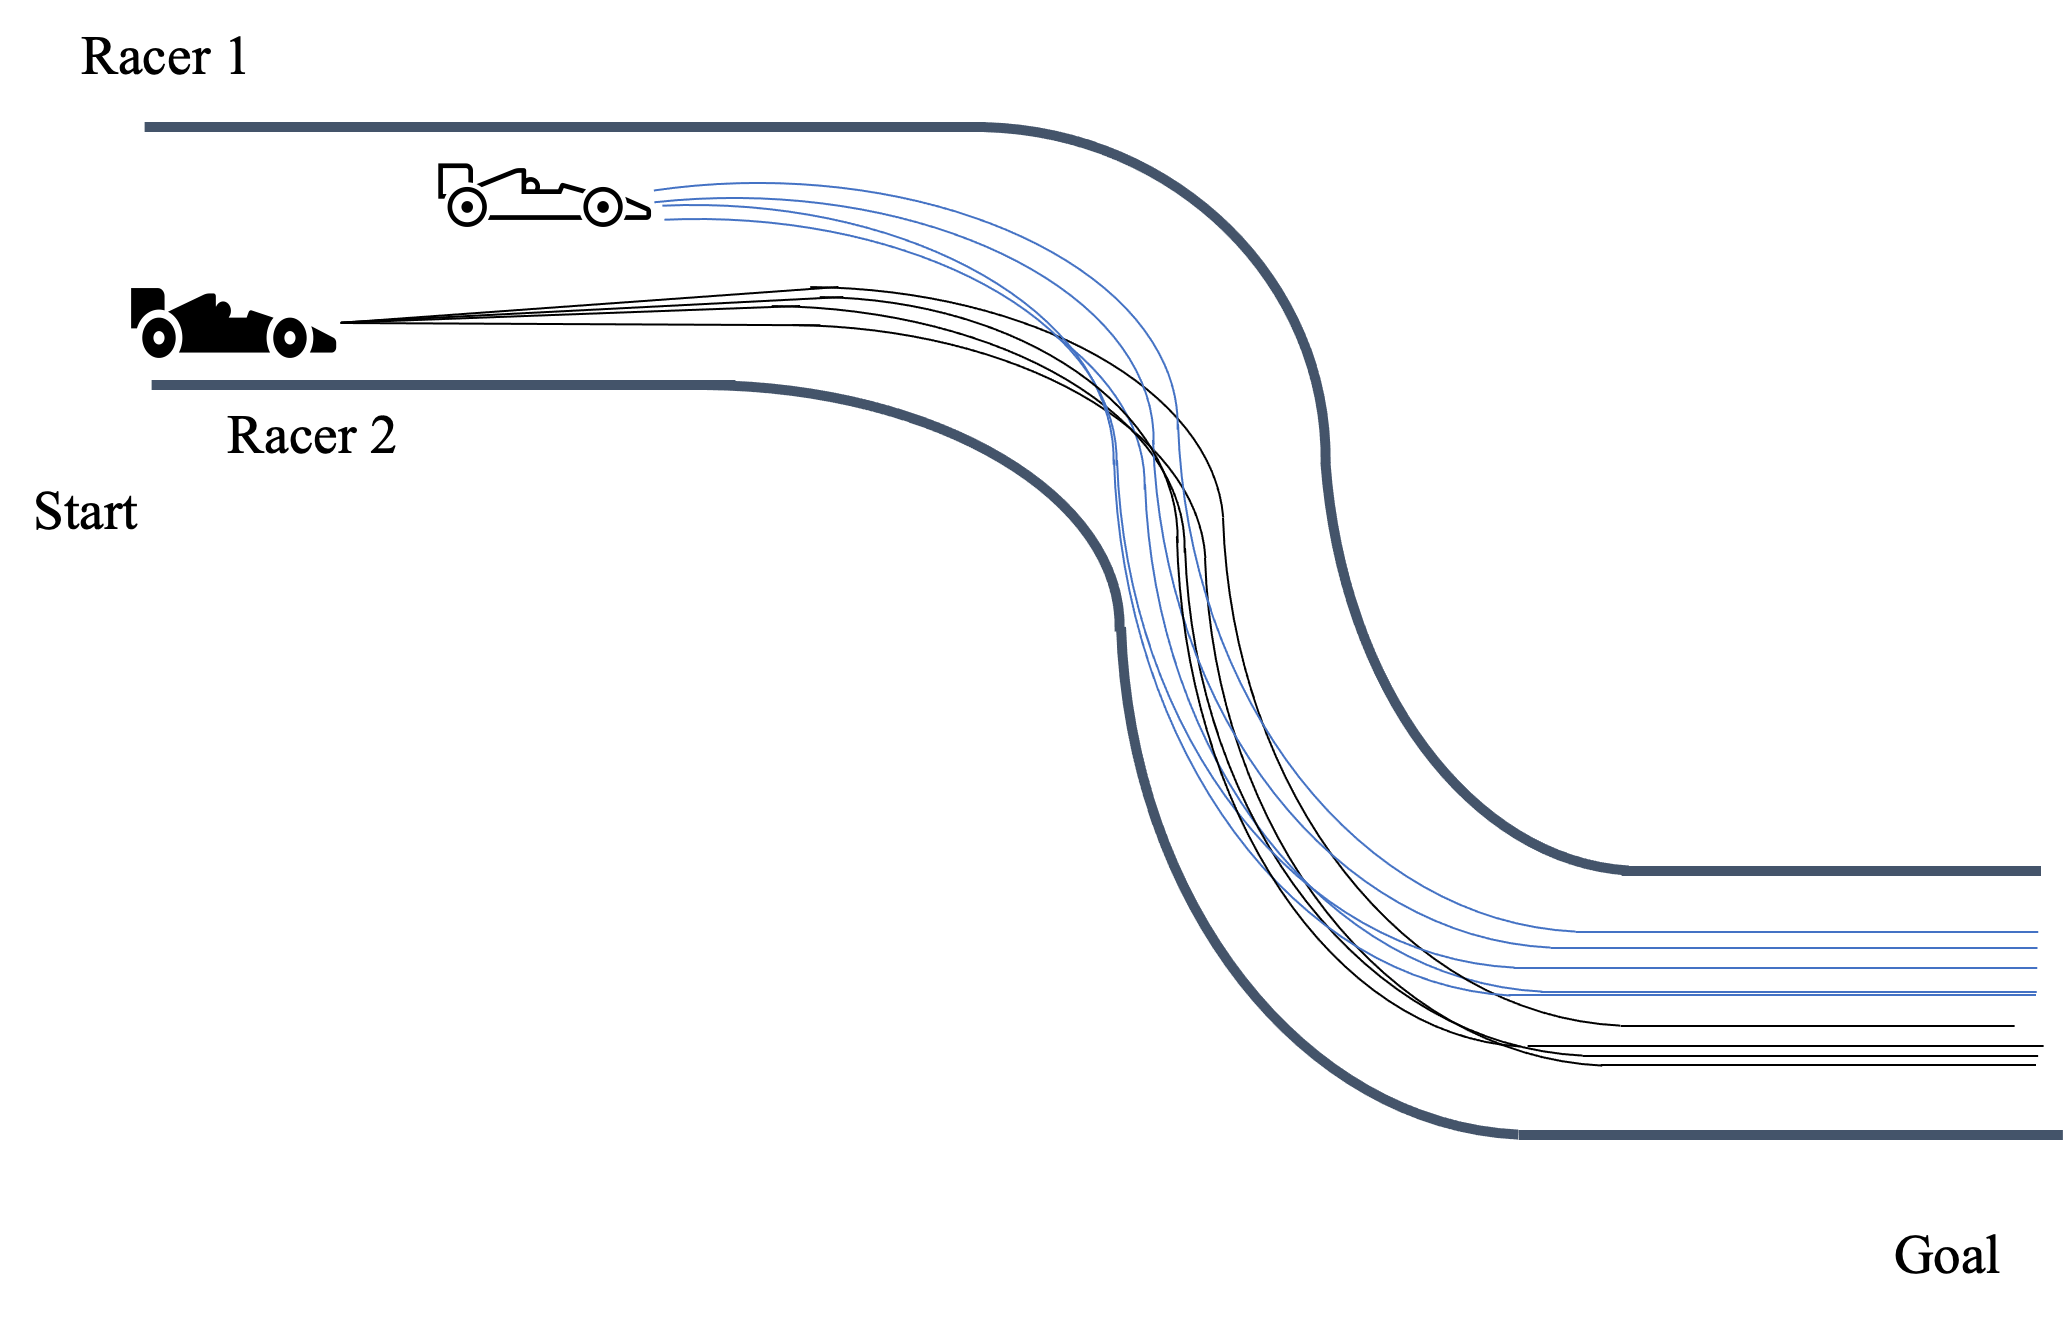
\includegraphics[width=0.75\textwidth]{Figures/MotivatingExampleInfTraj.png}
\caption{Uncountably infinite trajectories to consider in racing.}
\label{fig:motivating_example:inf}
\end{center}
\end{figure}

In addition, prior work is also mainly focused on single-agent control or situations with agents who behave as stationary or dynamic obstacles rather than adversaries \cite{Liniger2014, Anderson2016, Kalaria2021, Kloeser2020,OKelly2020, Vazquez2020, He2021, Hou2016, Stahl2019_2}. However, when we hear the term ``racing," we naturally think of it as multi-agent game where all participants are competing against one another. Although it is possible to introduce adversarial objectives and constraints in the optimization-based control methods, they are prone to computational limitations in terms of planning horizon or control frequency for direct low-level control \cite{Liniger2020, Li2021}. Consider the simple scenario in Figure \ref{fig:motivating_example:inf}. There is an infinite number of trajectories that the black car might use to overtake the white car across the next two turns on a track. In order to use existing methods, we must compromise by either shortening the planning horizon and/or simplifying the objectives or constraints in the model. With a short horizon, it is just infeasible to plan for the medium-term to long-term strategic decisions to successfully overtake. Otherwise, if the model is simplified, we may no longer have an accurate representation of the game's rules or dynamics. With either compromise we lose the ability to perform the long-term game theoretic reasoning.

\begin{figure}
\begin{center}
   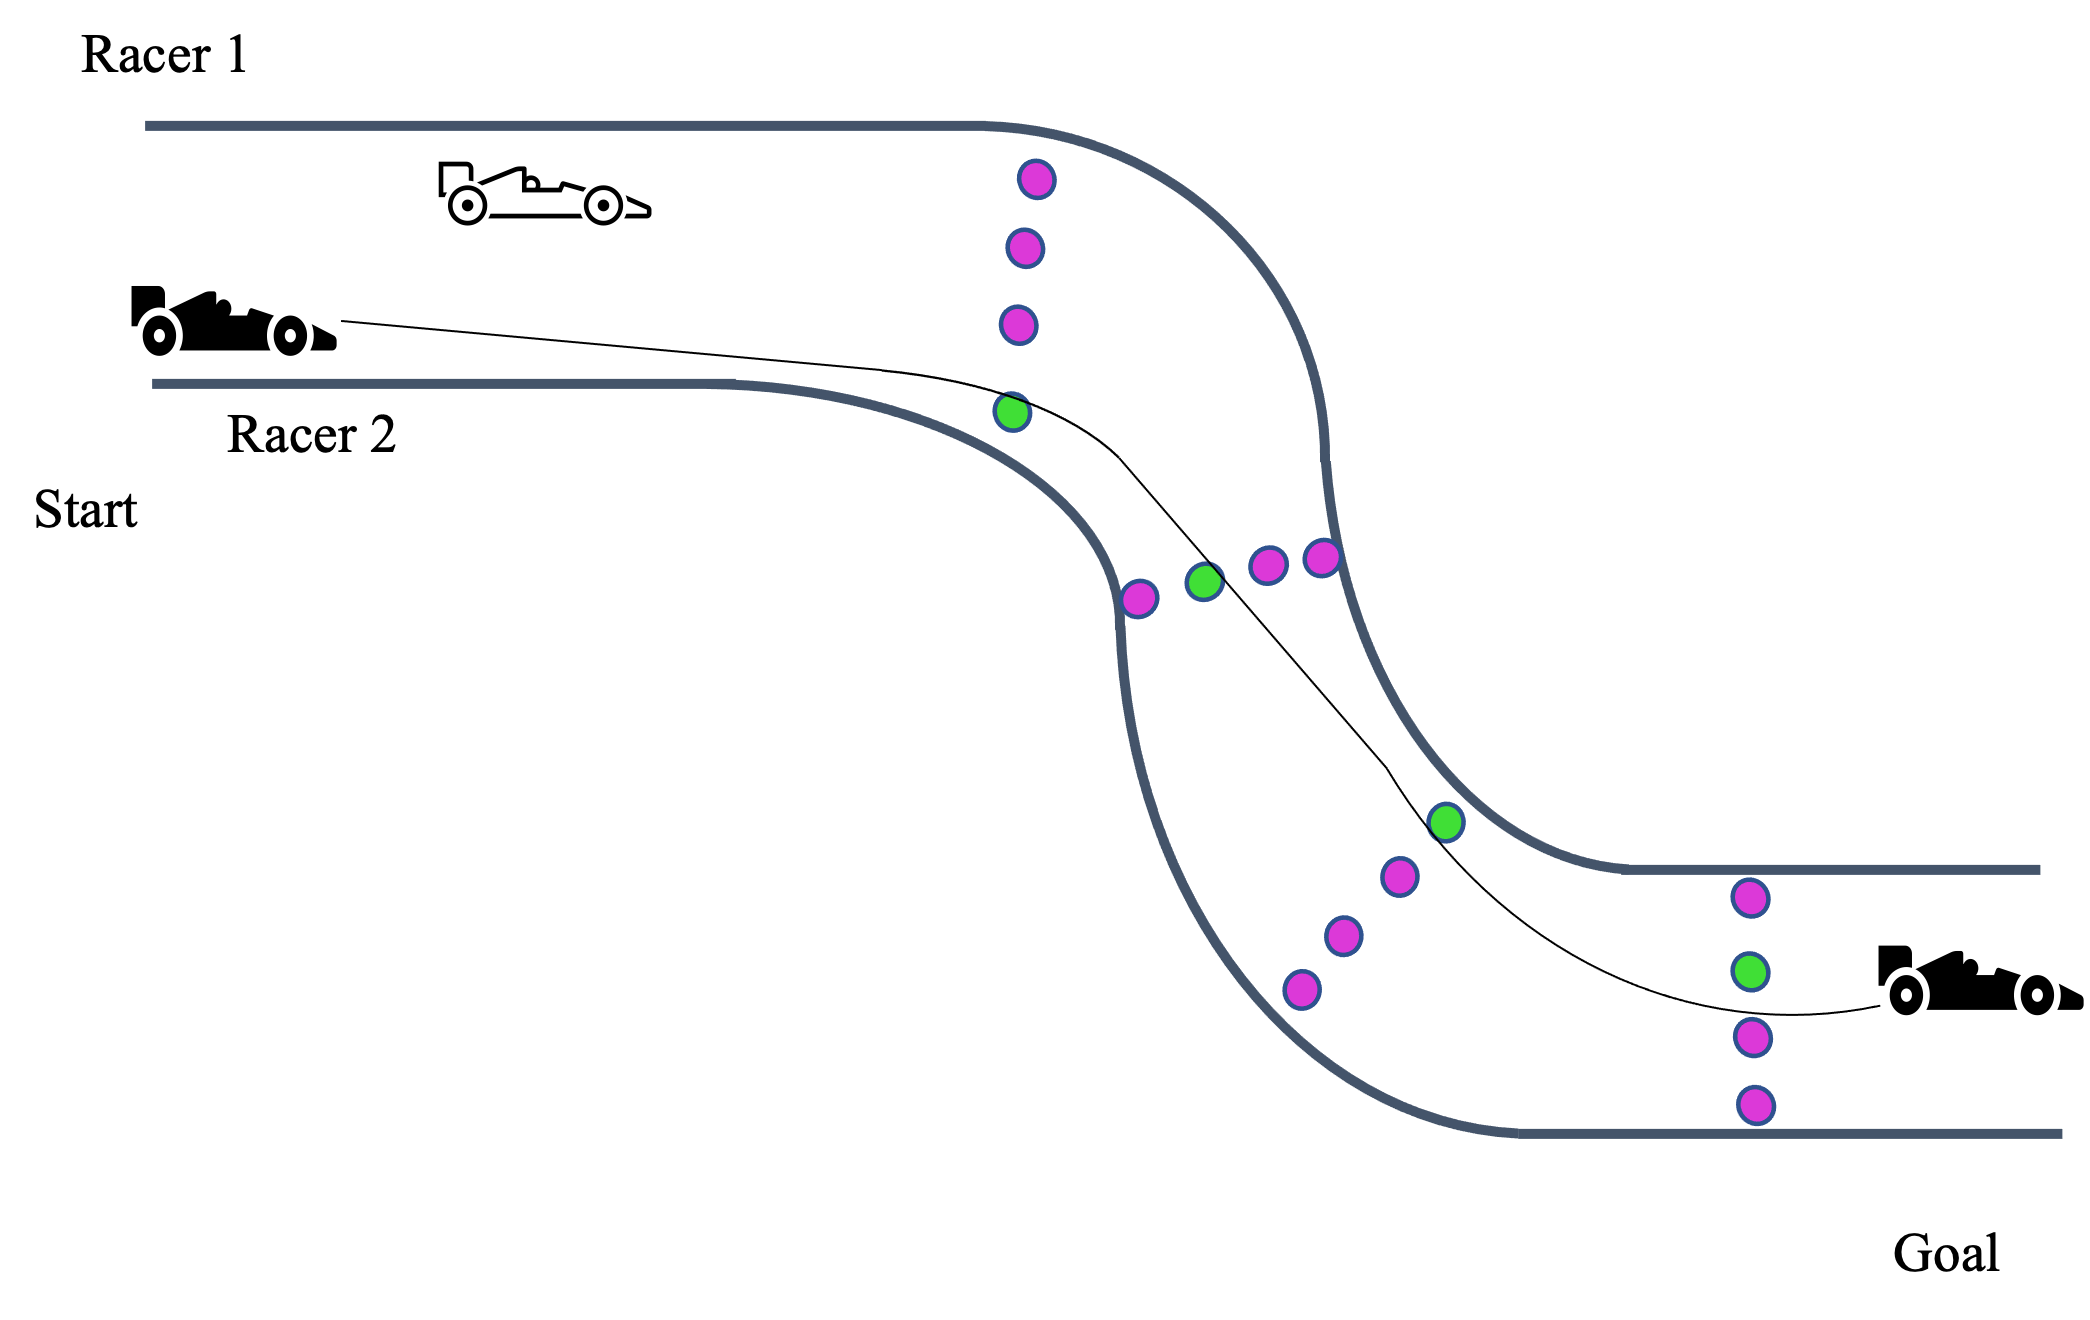
\includegraphics[width=0.75\textwidth]{Figures/MotivatingExampleOracle.png}
\caption{A high-level plan outlining lane choices (green) followed by a single trajectory (black).}
\label{fig:motivating_example:oracle}
\end{center}
\end{figure}

Therefore, practical implementation of such a complex control application suggests breaking down the system into layers of hierarchical reasoning (Figure \ref{fig:motivating_example:oracle}). There are effectively four high-level decisions to make in this scenario located at the first turn entry, the first turn exit the second turn entry, and the second turn exit. The domain of these decisions involves determining which of the four lanes to be positioned at each of the locations. If there is an oracle that can determine the ideal choice of lane for those locations such that the rules and dynamics are satisfied, highlighted in green, the problem for our precise, low-level controller becomes much simpler. It no longer needs to decide both where to be positioned and how to move between those positions; rather, is just a matter of calculating the latter. 

\section{Contributions} %td
This report develops a hierarchical control scheme that reasons about optimal long-term plans and adheres to the safety and fairness rules seen in real-life multi-agent racing. We provide a general formulation for a multi-agent racing game that encodes these complex rules and study the problem in three parts.

In the first part, we construct a turn-based, discrete simplification of a racing game that encapsulates the discrete nature of the safety and fairness rules from the general formulation. We outline temporal logic specifications to represent these rules and use the specifications to rule out players' choices in the game. Furthermore, we develop a turn-based mechanism to preserve the realistic flow of information that would occur in a continuous setting. Our resulting discrete game has a simple reachability objective over a finite number of steps, which is solved using value iteration. We evaluate our formulation by considering three case studies of common racing scenarios. 

In the second part, we use construct the full hierarchical control scheme for head-to-head racing that runs in real-time. We use the discrete game formulation from the first part as the high-level planner and use Monte Carlo tree search to solve the game in real-time. The solution of the discrete formulation effectively produces a series of long-term waypoints that are safe with respect to the rules and approximately optimal. Then, we formulate a simplified version of the general racing game to track the waypoints with relaxed representations of the original rules. The simplified game is solved using two methods to produce high-resolution control inputs: training a policy using multi-agent reinforcement learning and solving a linear-quadratic Nash game approximation. Our structure yields a pair of hierarchical controllers that run in real-time and outperform baselines resembling previously studied autonomous racing methods in terms of head-to-head performance and obedience for following safety rules. Moreover, our controllers produce behavior resembling that of expert human drivers. 

In the final part, we consider an extension of head-to-head racing by introducing team-based objectives, which is a major part of real-life competitions. To our knowledge, this is the first work to study a mix of cooperative and competitive objectives for coalitions of players in multi-agent racing. We generalize each of our game formulations from the previous sections by updating the objectives to evaluate the performance of one or more players on a team while subject to the same rules and constraints. Then, we use our proposed hierarchical control structure and compare them with the baseline methods adapted to play the updated form of the game. Our controllers show impressive performance compared to the baselines although the game has become more complex. Again, our controllers exhibit tactics resembling human experts.

Although this hierarchical control method is developed in the context of a racing game, the structure of the proposed architecture effectively reasons about optimal choices in a game-theoretic setting with complex constraints involving temporal logic and both continuous and discrete dynamics. As a result, we can apply this method to many other competitive settings that exhibit the aforementioned properties such as financial systems, power systems, or traffic control systems.

\section{Outline}
The remainder of this report is organized as follows. 
% Chapter \ref{chapter:prelim} summarizes some preliminaries for this report. 
Chapter \ref{chapter:litreview} provides a literature review of prior research in autonomous racing. 
Chapter \ref{chapter:synthesis} introduces the general racing game formulation, and outlines the discrete game abstraction of the general formulation. 
Chapter \ref{chapter:hier} develops the full hierarchical control scheme by utilizing the discrete formulation from the previous chapter as a high-level planner and constructing low-level formulation. 
Chapter \ref{chapter:team} applies the hierarchical controller to a team-based multi-agent racing. 
Finally, Chapter \ref{chapter:conclusion} concludes this work by providing a summary and ideas for further extensions. 
% \chapter{Preliminaries} \label{chapter:prelim}
\section{Dynamic Games} %td
\subsection{Discrete Dynamic Games} %td
\subsection{Monte-Carlo Tree Search Methods} %td
\subsection{Linear-Quadratic Games} %td
\section{Reinforcement Learning} %td
% https://stable-baselines3.readthedocs.io/en/master/modules/ppo.html
\subsection{Proximal Policy Optimization} %td
\subsection{Self-Play} %td
\subsection{Counterfactual Multi-Agent Policy Gradients} %td
\section{Temporal Logic} %td


\chapter{Literature Review} \label{chapter:litreview}
There are many components in the pipeline to build a complete autonomous racing system such as perception, planning, control, and hardware integration, all of which have a rapidly growing collection of literature \cite{litreview}. However, the focus of this report and literature review is limited to planning and control. Most prior work in autonomous racing control is focused on single-agent lap time optimization because multi-agent racing is an inherently more complex problem. Nevertheless, there are recent developments in multi-agent racing, but they are limited in the rules being modeled from real-life racing. They primarily focus on basic collision avoidance. In reality, certain players bear more responsibility for collision avoidance depending on the state of the game, and there exist additional rules on lane changes to ensure safety and fairness. Finally, we also study prior works using hierarchical reasoning to solve challenging problems in several contexts of autonomous driving. 

\section{Single-Agent Racing} 
Single-agent racing approaches utilize a mixture of optimization and learning-based methods primarily focusing on finding and tracking the optimal racing trajectory that minimizes lap time. \citet{Hou2016} use Monte Carlo tree search to estimate where to position the car around various shaped tracks to define an optimal trajectory. \citet{Vazquez2020} propose a method that computes an optimal trajectory offline and uses a model predictive control (MPC) algorithm to track the optimized trajectory online . Similarly, \citet{Stahl2019_2} also perform calculations offline by creating a graph representation of the track to compute a target path and use spline interpolation for smooth online path generation in an environment with static obstacles . Lastly, several studies use variants of MPC depending on dynamics model of choice and numerical optimization methods such as sequential quadratic programming or stochastic optimization algorithms \cite{Liniger2014, Anderson2016, Kalaria2021, Kloeser2020,OKelly2020}.  

In the category of learning-based approaches, \citet{Kabzan2019} develop an online learning algorithm to update parameters of an MPC-based controller using on feedback from applying control inputs. \citet{Remonda2021} use deep reinforcement learning to train a neural network policy with vehicle telemetry data. However, their experiments indicate that the method does not generalize when extended to tracks the model is not trained on. \citet{deBruin2018} use state representation to improve the generalization of the reinforcement learning based control for racing on unseen tracks. Finally, \citet{weiss2020} develop a deep-learning framework that uses vision to estimate waypoints in a player's local space track them using optimization-based control methods.

\section{Multi-Agent Racing}
In multi-agent racing studies, both optimization and learning-based control approaches are also used. \citet{Liniger2020} formulate and solve bimatrix games for three types of common scenarios in head-to-head racing but do not apply it to a real-time system. \citet{Li2021} use mixed-integer quadratic programming formulation with realistic collision avoidance. However, they concede that this formulation struggles to run in real-time due to the computational complexity of solving integer programs. \citet{spica2020real} propose a real-time control mechanism for a game with a pair of racing drones. This work provides an iterative-best response method while solving an MPC problem that approximates a local Nash equilibrium. It is eventually extended to automobile racing and multi-agent scenarios with more than two players by Wang et al. \cite{Wang2019, Wang2021}. \citet{He2021} create a fast, real-time MPC algorithm to make safe overtakes, but their method does not consider adversarial behavior from the opposing players . 

Next, we outline some of the learning based multi-agent racing works. Schwarting et al. train a policy using vision-based deep learning and self-play to predict opponent states that outperforms a model that independently learns to predict opponent behaviors \cite{Schwarting2021}. Their policy produces behavior mimicking human racing drivers. Song et al. use curriculum learning to train a policy that iteratively builds its knowledge from single-agent racing to overtaking and finally to collision avoidance \cite{Song2021}. Again, these approaches do not consider racing rules other than simple collision avoidance. 

\citet{sonyai} develop an autonomous racing controller using deep reinforcement learning that considers the rules of racing beyond just simple collision avoidance. Their controller outperforms expert humans while also adhering to proper racing etiquette. It is the first study to consider nuanced safety and fairness rules of racing and does so by developing a reward structure that trains a controller to understand when it is responsible for avoiding collisions, and when it can be more aggressive.  

\section{Hierarchical Control}
Hierarchical reasoning is a method that has also been previously studied in various contexts for autonomous driving. \citet{LinigerThesis} outlines a hierarchical racing controller that constructs a high-level planner with simplified dynamics to sample sequences of constant curvature arcs and a low-level planner to use MPC to track the arc that provided the furthest progress along the track. \citet{Fisac2019} develop a two-level planning system to control an autonomous vehicle in an highway environment with aggressive human drivers. The upper-level system produces a plan to be safe against the uncertainty of the human drivers in the system by using simplified dynamics. The lower-level planner implements the strategy determined by the upper level-planner using precise dynamics. Similarly, \citet{Moghadam2019} study hierarchical reasoning for sequential decision making in highway driving. They construct a high-level planner using a trained reinforcement-learning policy to determine lane changing plans to safely pass other drivers. The lane changing plans are shared with low-level controllers to execute those actions. Finally, \citet{Wongpiromsarn2012} develop a reactive synthesis and hierarchical control approach where an urban driving agent's objective is defined by a series of temporal logic specifications. Their hierarchical control system has an upper level that selects target states to reach and a lower level that implements plans to reach those states in order to ensure the specifications are met.
\chapter{Synthesis of Verifiably Safe and Optimal Racing Maneuvers using Temporal Logic Specifications}
% \epigraph{\flushright The Pledge}{}
\epigraph{\flushright The first part is called "The Pledge". The magician shows you something ordinary \ldots he asks you to inspect it to see if it is indeed real, unaltered, normal. But of course... it probably isn't.}{Christopher Priest}
\label{chapter:synthesis}
\section{General Multi-Agent Racing Game Formulation} \label{section:genform}
To motivate our discretized game approximation, we begin by outlining a general multi-agent racing game formulation involving rules seen in real-life racing. 

% Table \ref{tab:gen_symbols} lists all of the variables and functions referenced in the formulation. 
Let there be a set, $N$, of players racing over $T$ steps in $\mathcal{T} = \{1, ..., T\}$. There is a track defined by a sequence of $\tau$ checkpoints along the center, $\{c_i\}_{i=1}^{\tau}$, whose indices are in a set $C=\{1,..., \tau\}$. The objective for each player $i$ is to minimize its pairwise differences of the time to reach the final checkpoint with all other players. In effect, the player targets to reach the finish line with the largest time advantage. The continuous state (such as position, speed, or tire wear) for each player, denoted as $x^i_t \in X \subseteq \mathbb{R}^n$, and control, denoted as $u^i_t \in U \subseteq \mathbb{R}^k$, are governed by known dynamics $f^i$. We also introduce a pair of discrete state variables $r^i_t \in C$ and $\gamma^i \in \mathcal{T}$. The index of the latest checkpoint passed by player $i$ at time $t$ is $r^i_t$, and it is computed by function $p: X\rightarrow C$. The earliest time when player $i$ reaches $c_\tau$ is $\gamma^i$. Using these definitions, we formulate the objective \eqref{eq:gen_obj} and core dynamics \eqref{eq:gen_dyn}-\eqref{eq:gen_goal_time} of the game as follows:

\begin{equation} \label{eq:gen_obj}
    \min_{u^i_0, ..., u^i_T} (|N|-1)\gamma^i - \sum^N_{j \neq i}\gamma^j \\
\end{equation}

\begin{equation} \label{eq:gen_dyn}
    x^j_{t+1} = f(x^j_t, u^j_t), \quad \forall \;\; t \in \mathcal{T}, j \in N
\end{equation}
\begin{equation} \label{eq:gen_idx_map}
    r^j_{t+1} = p(x^j_{t+1}, r^j_t), \quad \forall \;\; t \in \mathcal{T}, j \in N
\end{equation}
\begin{equation} \label{eq:gen_init_idx}
    r^j_{1} = 1, \quad \forall \;\; j \in N
\end{equation}
\begin{equation} \label{eq:gen_reach_goal}
    r^j_{T} = \tau, \quad \forall \;\; j \in N
\end{equation}
\begin{equation} \label{eq:gen_goal_time}
    \gamma^j = \min \{t \, | \, r^i_t = \tau \wedge t \in \mathcal{T} \}, \quad \forall \;\; j \in N
\end{equation}

In addition to the core dynamics of the game, there are rules that govern the players' states. To ensure that the players stay within the bounds of the track we introduce a function, $q: X \rightarrow \mathbb{R}$, which computes a player's distance to the closest point on the center line. This distance must be limited to the width of the track $w$. Therefore, for all $t \in \mathcal{T}$ and $j \in N$:
\begin{equation} \label{eq:gen_idx_dist}
    q(x^j_{t}) \leq w
\end{equation}

Next, we define the collision avoidance rules of the game. We use an indicator function that evaluates if player $i$ is ``behind" player $j$. Depending on the condition, the distance between every pair of players, computed by function the $D: X \rightarrow \mathbb{R}$, is required to be at least $s_1$ if player $i$ is behind another player $j$ or $s_0$ otherwise. Moreover, because following players have a greater collision avoidance responsibility than leading players, $s_1 \geq s_0$. For all $t \in \mathcal{T}$, $j \in N$, and $k \in N \setminus \{j\}$ these rules are expressed by the constraint:
\begin{equation} \label{eq:gen_coll_avoid}
    D(x^j_{t}, x^k_t) \geq  \begin{cases} s_1 & \mathds{1}_{\text{player} \, i \, \text{behind player}\,j} \\
    s_0 & \text{otherwise}  \end{cases}
\end{equation}

Finally, players are limited in how often they may change lanes depending on the part of the track they are at. We assume that there are $\lambda \in \mathbb{Z^+}$ lanes across all parts of the track. If the player's location on the track is classified as a curve, there is no limit on lane changing. However, if the player is at a location classified as a straight, it may not change lanes more than $L$ times for the contiguous section of the track classified as a straight. We define a set $\mathcal{S}$ that contains all checkpoint indices where a player is located at a straight section. We also introduce a function $z: X \rightarrow \{-1, 1, 2, ..., \lambda\}$ that returns the lane ID of a player's position on the track or $-1$ if the player is off-track. Using these definitions, we introduce a variable $l^j_t$ calculated by the following constraint for all $t \in \mathcal{T}$ and $j \in N$:
\begin{equation} \label{eq:gen_lane_var}
    l^j_{t} =  \begin{cases} l^j_{t-1} + 1 & \mathds{1}_{r^j_t \, \in \mathcal{S}} = \mathds{1}_{r^j_{t-1} \in \mathcal{S}}\wedge z(x^j_t) \neq z(x^j_{t-1}) \\
    0 & \text{otherwise}  \end{cases}
\end{equation}
This variable effectively represents a player's count of ``recent'' lane changes over a sequence of states located across a contiguous straight or curved section of the track. However, the variable is only required to be constrained if the player is on a straight section of the track. Therefore, the following constraint must hold for all $t \in \mathcal{T}$ and $j \in N$ and if $r^j_t \, \in \mathcal{S}$:
\begin{equation} \label{eq:gen_lane_lim}
    l^j_{t} \leq  L
\end{equation}
% Table of Symbols
% \begin{table} [!b]
% \centering
% \caption{Symbols in general formulation}
% \begin{tabular}{p{0.15\linewidth}|p{0.75\linewidth}}  \label{tab:gen_symbols}
% Symbol & Value\\ 
% \hline
% $N$ & Set of players in the game \\
% $\mathcal{T}$ & Set of steps in the game \\
% $\delta$ & Number of steps in the game \\
% $\{c_i\}_{i=1}^{\tau}$ & Sequence of checkpoints \\
% $C$ & Set of checkpoint indices \\
% $x^i_t$     &   Continuous state of player $i$ at time $t$   \\
% $u^i_t$      &   Control input of player $i$ at time $t$    \\
% $f(x^i_t, u^i_t)$  &  Continuous dynamics of player $i$ \\ 
% $r^i_t$      &  Index of last checkpoint passed by player $i$ at time $t$ \\ 
% $\gamma^i$     &  Time when player $i$ passed last checkpoint \\     
% $p(x^i_{t+1}, r^i_t)$  &  Function computing index of last track checkpoint passed  \\     
% $q(x^i_{t+1})$   &  Function computing minimum distance to last track checkpoint passed \\
% $w$      &  track width \\     
% $b^{(i,j)}_t$ & Binary state variable indicating if player i is directly behind player j \\
% $v(x^i_t, x^j_t)$ & Function computing value of $b^{(i, j)}_t$ \\
% $d(x^i_t, x^j_t)$ & Function computing distance between player i and player j \\
% $s_0$ & Minimum distance safety margin if player is not directly behind another \\
% $s_1$ & Minimum distance safety margin if player is directly behind another  \\
% $\lambda$ & Number of lanes in the track \\
% $l^i_t$ & Integer state variable indicating player $i$'s recent lane changes at time $t$ \\
% $y(x^i_t)$ & Function evaluating if player i is on a straight or curve \\
% $z(x^i_t)$ & Function computing the lane of the track player is in\\
% $L$ & Upper bound on the number of recent lane changes a player is allowed
% \end{tabular}
% \end{table}

% Describe challenges of special constraints -> better modeled as a discrete game
Most prior multi-agent racing formulations \cite{Wang2019, Wang2021, Li2021} do not include the complexities we introduced through defining constraints \eqref{eq:gen_coll_avoid}-\eqref{eq:gen_lane_lim}. They usually have a similar form regarding continuous dynamics and discrete checkpoints \eqref{eq:gen_dyn}-\eqref{eq:gen_goal_time}, and their rules only involve staying on track \eqref{eq:gen_idx_dist} and collision avoidance with a fixed distance. However, in real-life racing, there do exist these complexities both in the form of mutually understood unwritten rules and explicit safety rules \cite{racingrules}. As a result, we account for two of the key rules that ensure the game remains fair and safe:
\begin{enumerate}
    \item There is a greater emphasis on and responsibility of collision avoidance for a vehicle that is following another \eqref{eq:gen_coll_avoid}.
    \item The player may only switch lanes $L$ times while on a straight section of the track \eqref{eq:gen_lane_var}-\eqref{eq:gen_lane_lim}.
\end{enumerate}

The first rule ensures that a leading player can make a decision without needing to consider an aggressive move that risks a rear-end collision or side collision while turning from the players that are following. This second rule ensures that the leading player may not engage in aggressive swerving or ``zig-zagging" across the track that would make it impossible for a player that is following the leader to safely challenge for an overtake. 

While functions may exist to evaluate these spatially and temporally dependent constraints in the formulation, their discrete nature suggests that they cannot be easily differentiated. Therefore, it is not possible to simply apply state-of-the-art optimization algorithms would not apply to produce optimal control inputs in real-time. 

\section{Discrete Game Formulation}
In order to design a controller that can solve the realistic racing game formulation in the previous section, we must use an alternative to traditional optimization-based control methods. We recognize that complexities in the formulation arise from constraints over discrete properties of the players' trajectories. This characteristic of the formulation suggests that constructing a discrete abstraction of the game is an appropriate method to estimate feasible trajectories. In the following sections, we describe some abstractions and their justifications to construct a turn-based discrete game approximation of the original formulation. 

\subsection{Abstraction of State Space} \label{section:discstate}
We begin by constructing the discrete abstraction of the state space from the original formulation. We do not explicitly specify any components of players' states when defining the original formulation because it is agnostic to the vehicle dynamics model being considered. However, including variables computed by constraints \eqref{eq:gen_idx_map} and \eqref{eq:gen_lane_var}, we assume each player's state in the original game at least consists of following five variables as they are the only ones encoded in our discrete state representation:
\begin{itemize}
    \item position
    \item velocity
    \item number of ``recent" lane changes
    \item tire wear
    \item last passed checkpoint index
\end{itemize}
In the following subsections, we describe how the aforementioned state variables are transformed to produce a discrete model of a player.

\subsubsection{Discrete Representation of Racetrack}
\begin{figure}
\begin{center}
   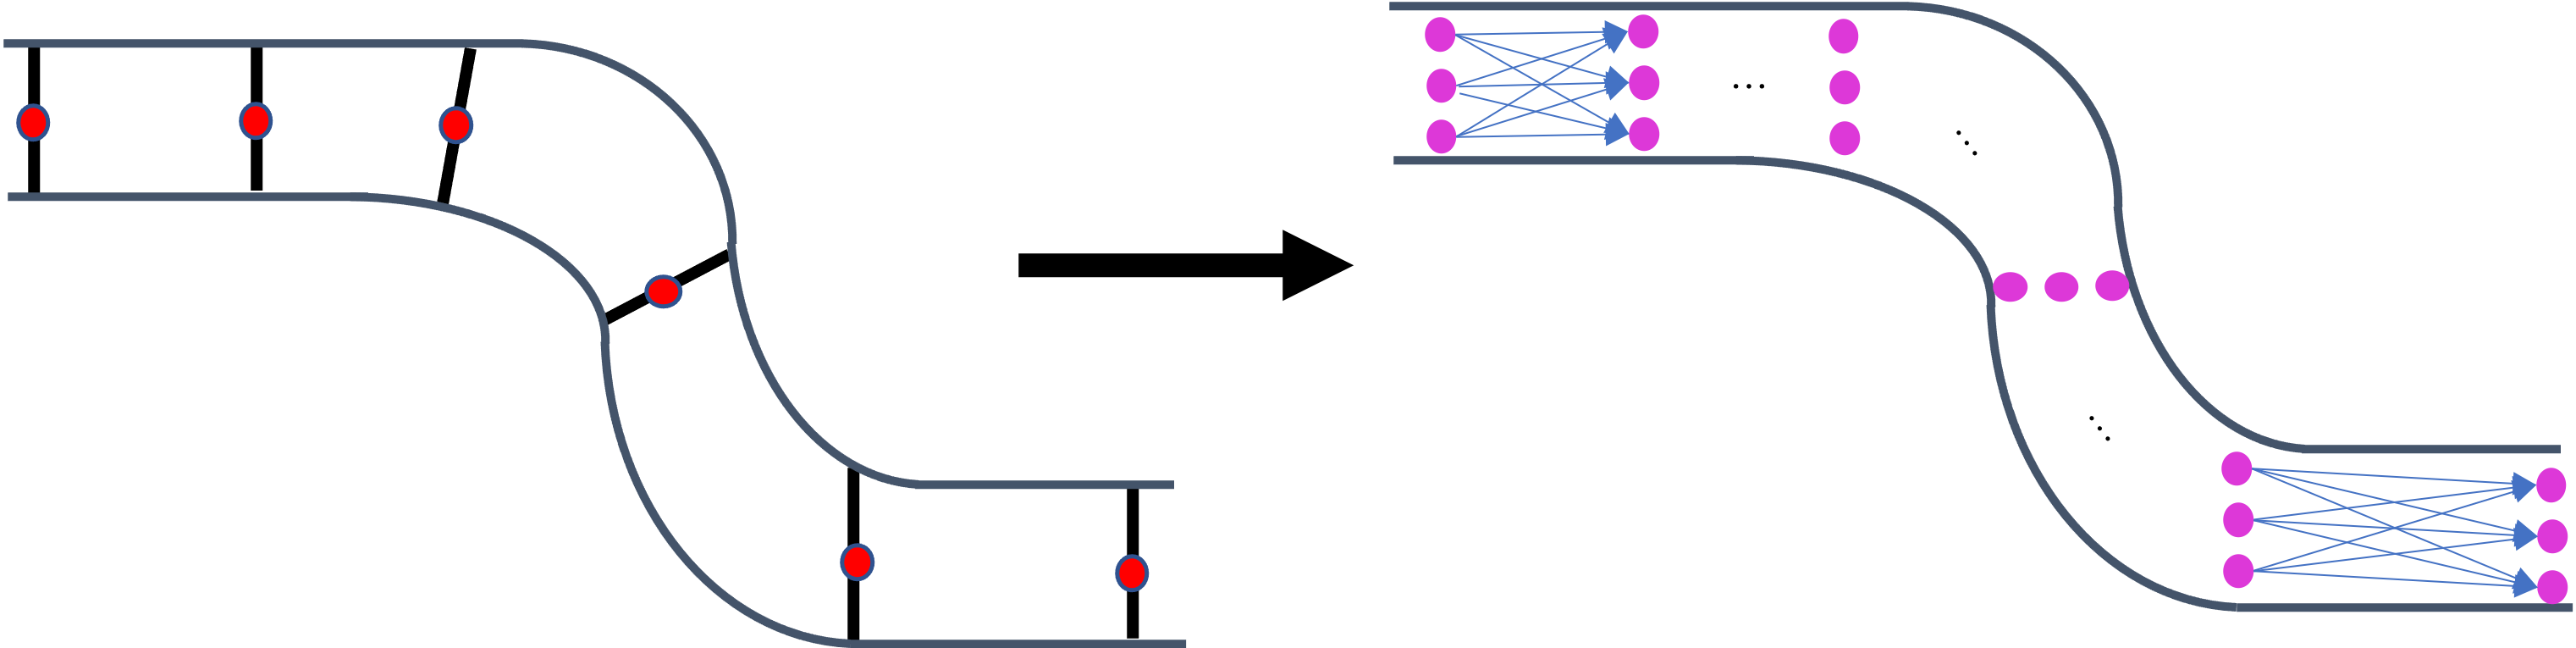
\includegraphics[width=\textwidth]{Figures/TrackAbstraction.png}
\caption[Transformation of racetrack in original formulation to discrete formulation.]{Transformation of the continuous race track with checkpoints (red) into discrete lanes at each checkpoint (purple).}
\label{fig:racetrack_abs}
\end{center}
\end{figure}
We change the mechanics so that the discrete game is played by making choices at the checkpoints that are indexed by $C$ rather than at each time-step from $\mathcal{T}$ defined in the original formulation. This transformation is natural to consider because all players must ultimately pass all checkpoints in order. As a result, the turns of the discrete game and players' states in the discrete game are indexed by their last passed checkpoint, and the time becomes a variable in the discrete game state. Furthermore, indexing by the checkpoints also produces a natural discretiziation for the position state variable in the original formulation. Around each checkpoint, we select $\lambda$ (which is the number of lanes) discrete locations along the line perpendicular to the direction of travel where each location evaluates to a unique lane ID on the track when passed into function $z(\cdot)$ defined in the general formulation. Therefore, we represent a player's position in discrete game formulation by its lane ID and index of the game state, i.e., the last passed checkpoint. This choice allows us to naturally encode the rules governing players' lanes and ensures that every location considered in the discrete game remains within the bounds of the track. Figure \ref{fig:racetrack_abs} visualizes the continuous space of the track with checkpoints (in red) is transformed into discrete locations associated with a unique lane ID at each checkpoint (in purple). 

\subsubsection{Discrete Representation of Player States}
\begin{figure}
\begin{center}
   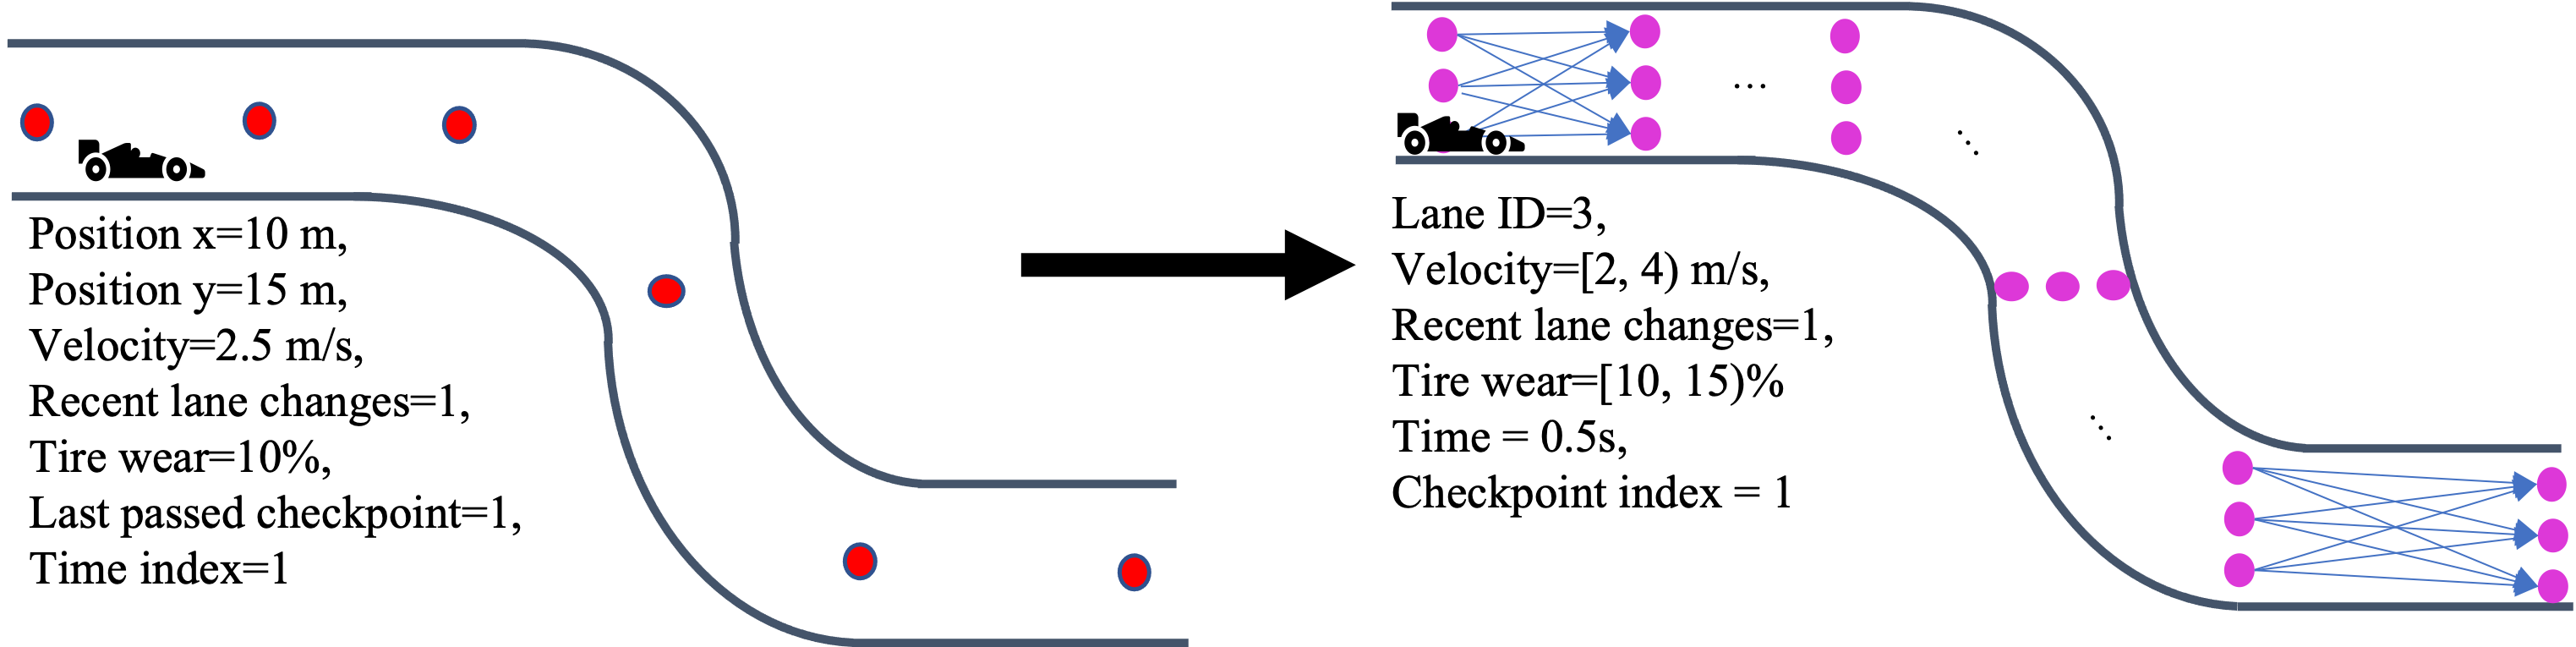
\includegraphics[width=\textwidth]{Figures/StateTransformation.png}
\caption{Transformation from original formulation state to discrete formulation state.}
\label{fig:state_transform}
\end{center}
\end{figure}
The remaining components of players' states are either already discrete valued, such as the count of ``recent lane changes," represented in the form of discrete buckets or rounded to a finite precision. For example, instead of considering real number value for a player $i$'s velocity from its state $x^i_v=\SI{2.5}{\meter\per\second}$ in the original game, the discrete representation would simply be $v^i \in [2, 4)\si{\meter\per\second}$. Figure \ref{fig:state_transform} visualizes a continuous state for a player converted into discrete form. The overall components of a player $i$'s discrete state are:
\begin{itemize}
    \item lane ID $a^i_k$
    \item velocity bucket $v^i_k$
    \item number of ``recent" lane changes $l^i_k$
    \item tire wear $e^i_k$
    \item time $t^i_k$
\end{itemize}
where $k$ is the index of the state and the checkpoint associated with the state. We also use the notation $k^i$ to refer to the index of the player $i$'s checkpoint in the overall game state because it is possible for the players' indices to be different as we are modeling a turn-based game.

\subsection{Abstraction of Dynamics} \label{section:discdyn}
Given discrete states of the players, we outline our abstraction of the dynamics, i.e. transitions between discrete states in the game. Because the discrete game is indexed by track checkpoint, we must also transform the players' control inputs. At each checkpoint, the players' choices are now the lane ID and target velocity bucket for the upcoming checkpoint. Next, we rewrite the constraints related to the racing rules in the original formulation as temporal logic specifications. We then discuss the specifics of how our state transitions are computed based on a given action and finish with describing the turn-based mechanism of the discrete formulation.

\subsubsection{Temporal Logic Specifications of Rules} 
Constraints regarding the rules of racing for player $i$ in the original transformation are now expressed as temporal logic specifications over the discretized state transformation:

\begin{enumerate}
    \item Stay on track \eqref{eq:gen_idx_dist}. To require that players stay on track we must ensure that the lane ID is within the subset of non-negative lane IDs.
    \begin{itemize}
        \item $\square \;  (a^i_k \in \{1, ..., \lambda\})$
    \end{itemize} 
    \item Avoid collisions \eqref{eq:gen_coll_avoid}. To abstract collisions, we require that players must always maintain a minimum time difference of $\mu$ if two players share the same lane ID at the same checkpoint. We assume that if there is a small time difference between the players at the same checkpoint and the same lane, there would be an increased risk of collision.
    \begin{itemize}
        \item $\square \;  ( \bigwedge_{j \in N \setminus i} (k^i=k^j \wedge a^i_k=a^j_k) \implies |t^i_k-t^j_k| \geq \mu))$
    \end{itemize}
    \item Limit lane changing on straights \eqref{eq:gen_lane_lim}. Ensure the ``recent" lane changes variable does not exceed $L$ if checkpoint index $k$ is a straight part of the track as represented by set $\mathcal{S}$ defined in the original formulation.
    \begin{itemize}
        \item $\square \; ((k \in \mathcal{S})  \implies (l^i_k \leq   L \; U \; k \notin \mathcal{S}))$
    \end{itemize} 
\end{enumerate}
The overall specification for each of the players is the conjunction of the list. Given our state discretization and action set, we could use synthesis methods to produce a controller to meet the specifications for some objective. However, the computational complexity of synthesizing a controller to meet such specifications is not manageable due to the exponential growth with respect to the number of specifications and variables \cite{Chen2013}. Therefore, we take advantage of the fact that most of these specifications are easily verified by simply examining a player's resulting state from a given state-action pair and that specification 1 is trivially satisfied by our state and action space abstraction (players are not allowed to choose target lanes outside of $\{1, ..., \lambda\}$). When constructing the model of the game, we simply disregard any player choice that violates the specifications thereby only considering states and trajectories that are allowed. 
\subsubsection{Computing State Transitions}
To check if a state-action pair satisfies the temporal logic specifications and the reasonably approximates vehicle dynamics, we must have a straightforward way of computing the resulting state variables when applying some action. 

Updating the lane ID and velocity states is trivial because it is the exactly the player's action. Similarly, updating the ``recent" lane changes variable is also simple with our state space design. We directly apply the logic from the original formulation \eqref{eq:gen_lane_var}. It only requires evaluating whether the track type classification of the pair of checkpoints is the same and if the choice of lane ID is different than the lane ID at the initial checkpoint. Therefore, if choosing an action implies that lane change limit $L$ is exceeded on the straight checkpoints, the action would be disregarded in model to satisfy specification 3. 

To calculate updates for the elapsed time state, we first use the known track parameters (such as turning radius or lane width) to estimate the distance to travel between the lane in the current checkpoint $c_k$ to the lane in the subsequent checkpoint $c_{k+1}$. If the track between two checkpoints is a straight, the Euclidian is used to estimate the distance to travel based on the lane width ($w_l$) and the distance between the location of the checkpoints $\gamma_{k, k+1}$. If the the track between the two checkpoints is a curve, then we calculate a coarse estimate of the distance by averaging the radius of the turn for player's lane at the initial checkpoint $r_k$ and radius of the turn for the player's target lane at next checkpoint $r_{k+1}$ and multiply it by the central angle of the turn $\theta_k$. These calculations are summarized below:

\begin{equation} \label{eq:dist_calc}
    d = \begin{cases}
    \sqrt{w_l^2 + \gamma_{k, k+1}^2} &  \text{if } k \in \mathcal{S} \\
    \frac{r_k + r_{k+1}}{2}\theta_k & \text{if } k \notin \mathcal{S}
    \end{cases}
\end{equation}

Given the estimated distance $d$, average velocity of bucket at the initial checkpoint $\bar{v}_k$ and average velocity of the target bucket $\bar{v}_{k+1}$ and parameters of the vehicle such as maximum allowed velocity $v_*$, maximum acceleration $a$, and maximum braking $b$, we use simple equations of motion to calculate minimum time it takes to travel the distance.  Moreover, maximum allowed velocity $v_*$ is estimated using the tire wear state at the initial checkpoint $e_k$, track radius, and the parameter of a vehicle's maximum allowed lateral acceleration. We enforce that $\bar{v}_{k+1} \leq v_*$ and disregard all actions that violate this requirement because such an action would not obey the lateral acceleration limitation of the vehicle. In addition, we verify it is possible to accelerate or decelerate from $v_k$ to $v_{k+1}$ within the distance if $v_k \leq v_{k+1}$ or $v_k \geq v_{k+1}$, respectively. If that is not possible, then the action with target velocity $v_{k+1}$ is also disregarded. For the remaining cases, we use the following calculation for the time update $\delta t_k$:

\begin{equation} \label{eq:time_update}
    \delta t_{k} = \begin{cases}
    \frac{v_*-\bar{v}_k}{a} + \frac{v_*-\bar{v}_{k+1}}{b} + \frac{d-\frac{v_*^2-\bar{v}_k^2}{2a} - \frac{v_*^2-\bar{v}_{k+1}^2}{2b}}{v_*} 
    &  \text{if } v_* \geq \bar{v}_k \; \wedge \\
     &\quad \frac{d-\frac{v_*^2-\bar{v}_k^2}{2a} - \frac{v_*^2-\bar{v}_{k+1}^2}{2b}}{v_*} \geq 0 \\
    \frac{\bar{v}_k -v_*}{b} + \frac{v_*-\bar{v}_{k+1}}{b} + \frac{d-\frac{\bar{v}_k^2 -v_*^2}{2b} - \frac{v_*^2-\bar{v}_{k+1}^2}{2b}}{v_*} 
    &  \text{if } v_* < \bar{v}_k \;\wedge \\
    &\quad \frac{d-\frac{\bar{v}_k^2 -v_*^2}{2b} - \frac{v_*^2-\bar{v}_{k+1}^2}{2b}}{v_*} \geq 0 \\
    \frac{\sqrt{\frac{-2dba -b\bar{v}_k^2 -a\bar{v}_{k+1}^2}{-a-b}}-\bar{v}_{k}}{a} + \frac{\sqrt{\frac{-2dba -b\bar{v}_k^2 -a\bar{v}_{k+1}^2}{-a-b}}-\bar{v}_{k+1}}{b}
    & \text{if } \bar{v}_k \leq v_* \\
    \text{action ruled out}
    & \text{otherwise}
    \end{cases}
\end{equation}

The calculation simply assumes the player accelerates or brakes to reach $v_*$ from $\bar{v}_k$, maintains that speed for as long as possible until the player must brake to hit $\bar{v}_{k+1}$ if $\bar{v}_{k+1} \neq v_*$. If there is not enough distance to perform this maneuver and $\bar{v}_k \leq v_*$, we calculate the highest velocity the player can hit given we must end at the target velocity within the specified distance. All other possible maneuvers would violate the dynamical limitations of the vehicle and are ruled out of the allowed actions. We also use the time state update to estimate collision avoidance and satisfy specification 2. If a player chooses a lane that a prior player has already selected for its turn and the difference in the time states for these players would be smaller than $\mu$ if the action is applied, then the action is disregarded.

Finally, in order to calculate the tire wear state update, we consider the straight and curve differently. If the track between the checkpoints is a straight, we multiply a tire wear factor parameter $L_{\text{straight}}$ for a straight with the distance of the straight $d$. When the track between the checkpoints is a curve, we multiply the tire wear factor parameter $L_{\text{curve}}$, the distance of the curve $d$, and an estimate for the average lateral acceleration achieved by hitting the target velocity $\bar{v}_{k+1}$ calculated using equations of circular motion. The tire wear update $\delta e_k$ is calculated as follows:
\begin{equation}
\delta e_k = \begin{cases}
    dL_{\text{straight}} & \text{if } k \in \mathcal{S} \\
    \frac{2dL_{\text{curve}}\bar{v}_{k+1}^2}{r_k + r_{k+1}} & \text{if } k \notin \mathcal{S}
\end{cases}
\end{equation}
For both the time and tire wear, the updates are added to the initial state and projected back into their discrete buckets or rounded to the finite precision.

Using these calculations, we have a way of computing the exact sequence of states given a sequence of player actions. Next, we discuss the final piece of our discrete game's dynamics by outlining the logic behind determining the order in which the players choose actions. 

\subsubsection{Turn-Based Mechanics}
Although players make decisions concurrently in the original game and real-life, our discrete abstraction is a modeled as a turn-based game. Because the states are indexed by the checkpoint instead of time, the game is played by evaluating the choices all players one checkpoint at a time. The order in which the players choose their actions at each checkpoint is determined by the player who has the smallest time state at the checkpoint being processed. A lower time state value implies that a player was at the given checkpoint before other players, so it would have made its choice at that location before the others in the continuous setting. This ordering also implies that players who arrive at a checkpoint after preceding players observe the actions of those preceding players preserving the realistic flow of information. Most importantly, because the ordering forces the following players to choose last, we also capture the rule that the following players (i.e. those that are ``behind'' others) are responsible for collision avoidance after observing the leading players' actions. As a result, in conjunction with satisfying specification 2, we model realistic collision avoidance rules. 

\subsection{Discrete Game Objective} \label{section:discobj}
The final component of our discrete game is the determining the rewards and the objective. The reward function for a player $i$ is: 
\begin{equation}
    R^i(s^1, ... s^n) = \begin{cases} 
                (\sum_{j \in N \setminus i} s^j_t) - |N-1|s^i_t & \text{if } (\bigwedge_{m \in N} s^m_k   = c_\tau) \\ 
                0    & \text{otherwise}
                \end{cases}
\end{equation}
It is zero for all states except the one after all players have reached the final checkpoint. At the final checkpoint, player $i$'s reward is the pairwise difference in the time state with each player after everyone has reached the goal, which resembles the original game formulation's objective \eqref{eq:gen_obj}. The objective for each player is to simply maximize this reward.

\subsection{Summary of Formulation}
Given the state space, dynamics, and objective of the game, we have effectively constructed a finite dynamic game. We write this game in a more general form as a stochastic multiplayer game (SMG) defined by Chen et al. as a tuple of the following elements \cite{Chen2013}:


\begin{itemize}
    \item $S$ is the finite state space of the game, which is the set product of all players and the domains of each of the state variables.
    \item $A^1(\boldsymbol{s}), \ldots, A^{|N|}(\boldsymbol{s})$ are the finite action sets of each of the players dependent on the current state, which includes full knowledge of the other player' state and the track position variable.
    \item $F^1(\boldsymbol{s}, a^1, \boldsymbol{s}'), \ldots, F^{|N|}(\boldsymbol{s}, a^{|N|}, \boldsymbol{s}')$ are the transition functions for each player following the calculations described previously.
    \item $R^1(\boldsymbol{s}),\ldots,R^{|N|}(\boldsymbol{s})$ are the reward functions provided in the prior section.
     \item $AP = \{\text{goal}\}$ atomic propositions.
    \item $L: S \rightarrow 2^{AP}$ is the labeling function for the states for the set $AP$. The function labels all states where all players have reached the final checkpoint with $\{\text{goal}\}$, and all other states with $\varnothing$.
\end{itemize}

Once in the SMG form, we can use state-of-the-art model checking tools with a simple reachability specification, $\lozenge \text{goal}$, to synthesize optimal strategies for the players to maximize their rewards. 
% Furthermore, we are guaranteed to find a pure strategy Nash equilibrium because we constructed a finite dynamic game. CITETHIS\footnote{\url{https://econ.uiuc.edu/~hrtdmrt2/Teaching/GT_2017_19/L3.pdf}}.

\section{Case Studies of Strategic Scenarios}
\begin{figure}
\begin{center}
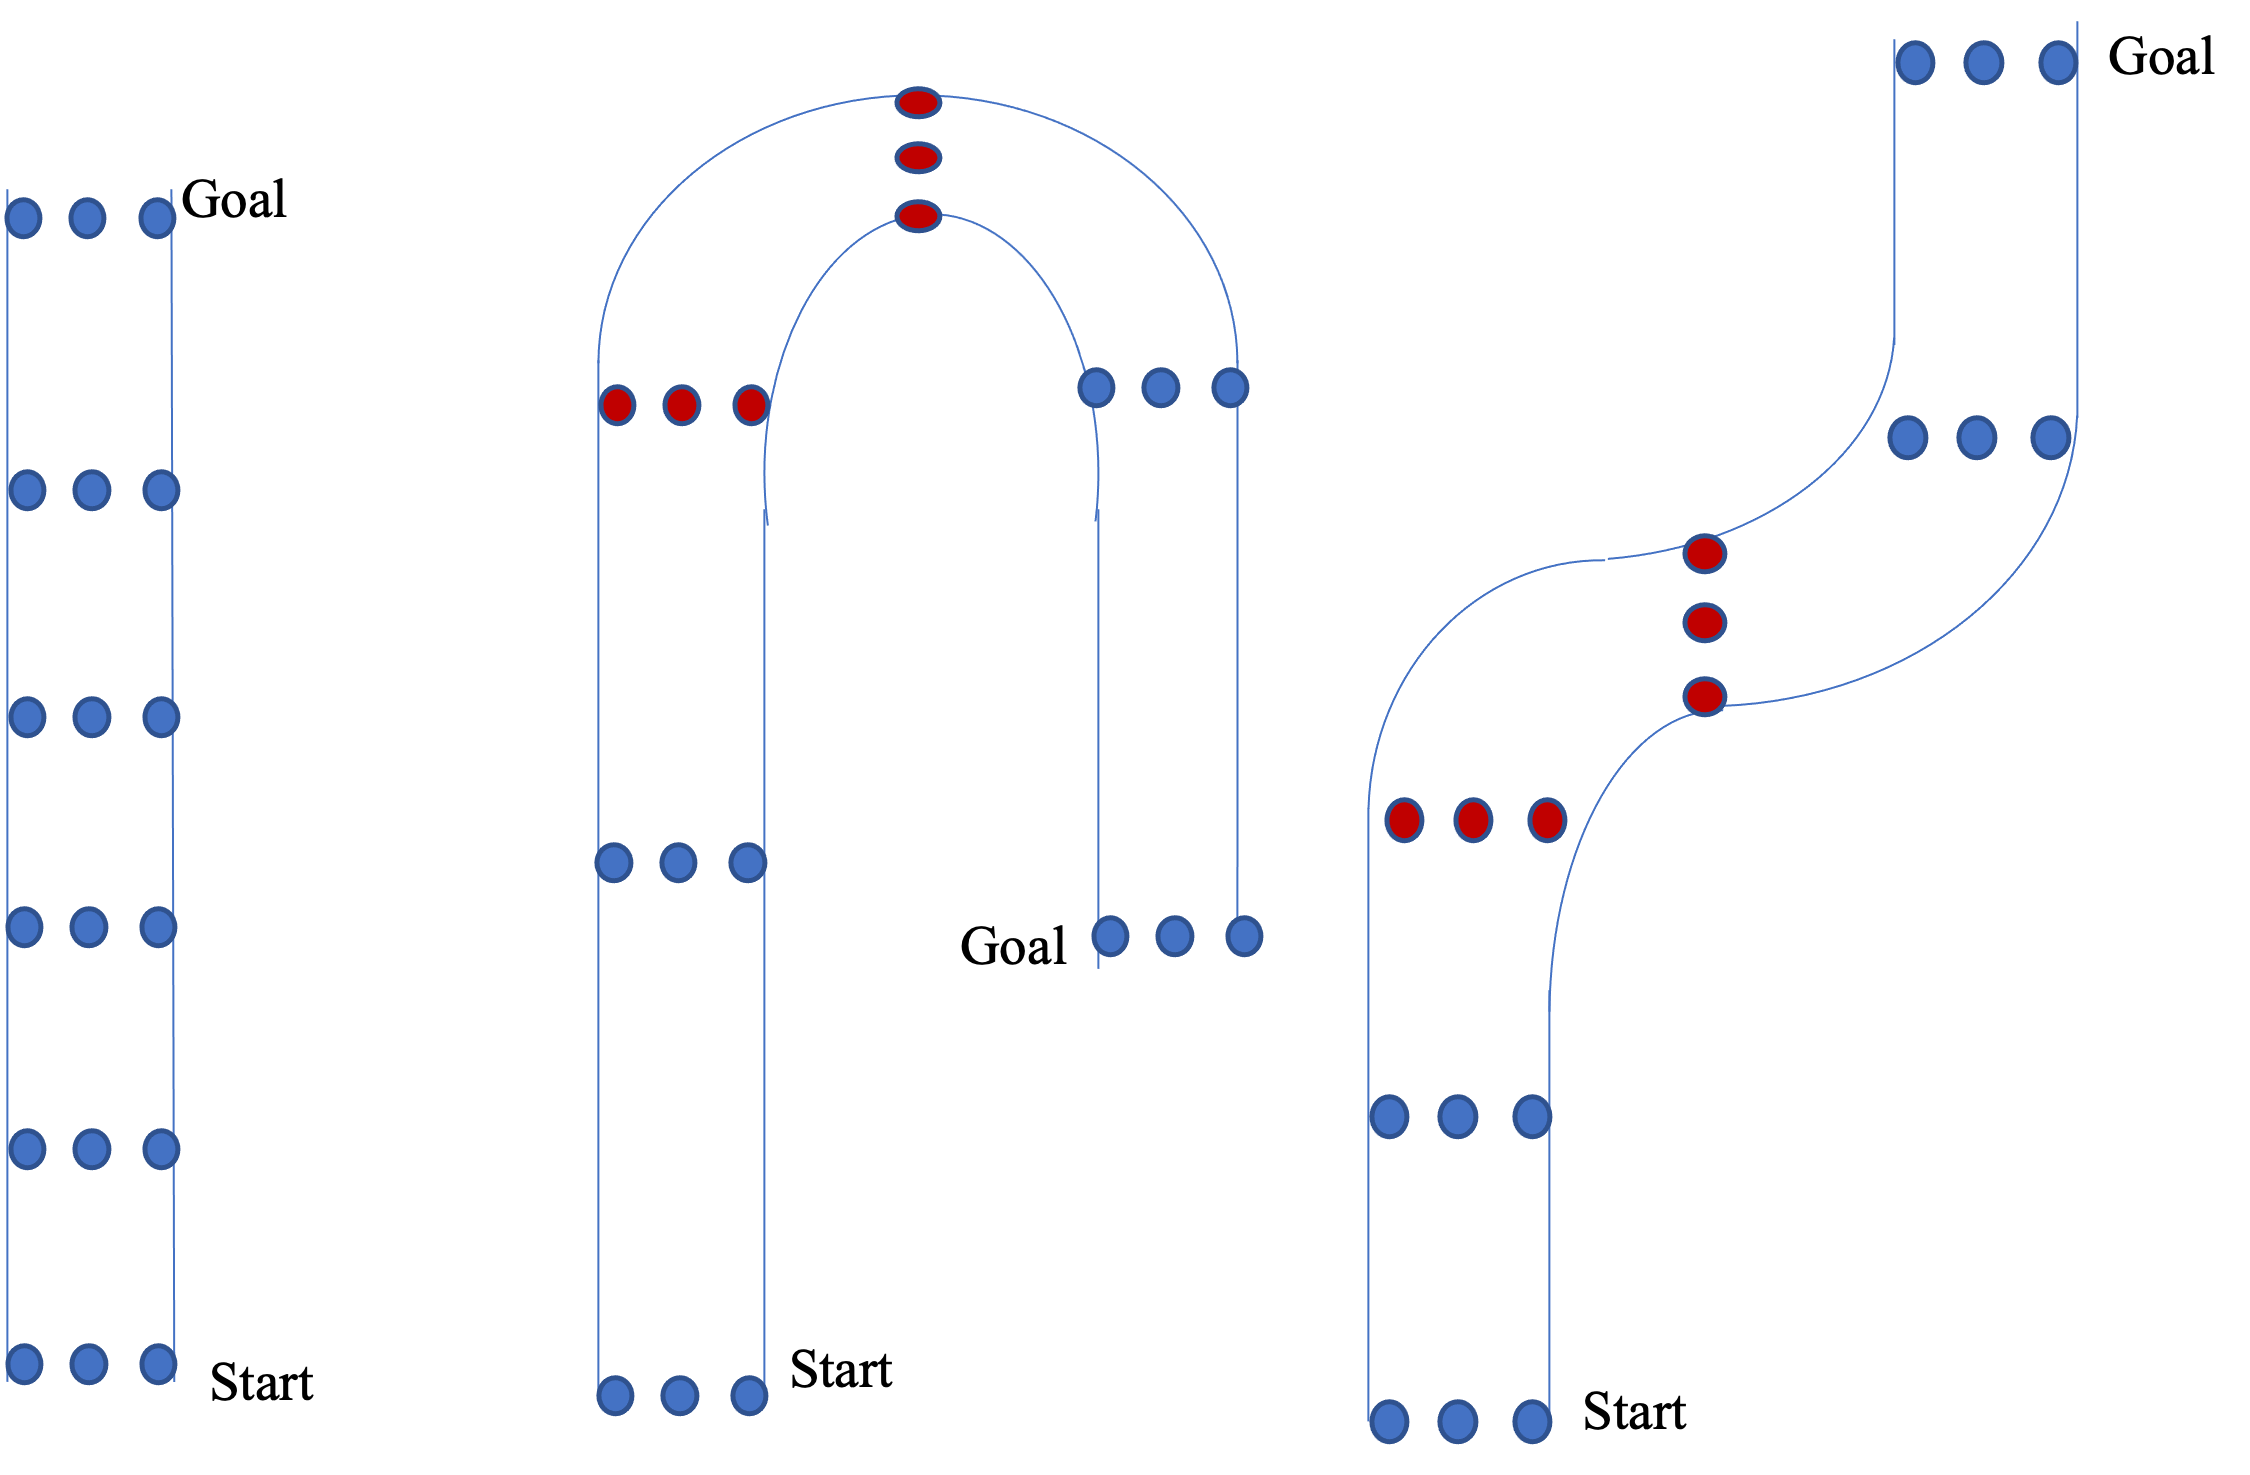
\includegraphics[width=\textwidth]{Figures/TrackShapes.png}
    \caption[Discrete representation of common track shapes.]{\label{fig:track_shapes} Three track types straight, hairpin, and chicane visualized from left to right. Each shape is discretized by 6 checkpoints and 3 lanes. The discrete nodes are color coded using their classification as straights (blue) or corners (red).}
\end{center}
\end{figure}
To evaluate if our discrete game formulation is a reasonable representation of real-life racing, we apply the model to several case studies resembling some common race scenarios for two players. The goal is to visualize and interpret the produced strategies to ensure it matches with our prior understanding of what might happen in a similar scenario in real-life racing. We categorize the scenarios based on three common types of track shapes: long straight, hairpin, and chicane shown in Figure \ref{fig:track_shapes}. For each of the track shapes, we explore various combinations of initial states for tire wear, velocity, and elapsed time for the players. We analyse the scenarios in the perspective of player 1 and start it with a non-zero time state for each study. Setting a non-zero initial time state indicates that it is starting with a disadvantage and is behind player 2. However, we analyze the initial states where player 1 is able to overtake player 2 or see what the best time gap it achieves. 

In order to make the results of the studies more interesting, we also assume that the players' vehicles have different dynamical parameters. Player 1 has a higher top speed than racer 2 but has a lower acceleration than racer 2. However, racer 2 has a higher limit for maximum lateral acceleration, which is used for computing maximum velocity allowed during turning, but it also has a higher tire wear factor. If both cars have the exact same configuration, the strategies of both vehicles would be similar. Furthermore, it would be near impossible for the player 1 to overtake the player 2 with perfect play. The exact parameters used when generating the transitions functions for each player is listed in Table \ref{table:params}.

\begin{table}
\resizebox{\textwidth}{!}{%
\begin{tabular}{|l|l|l|}
\hline
\textbf{Vehicle Parameter}                                                                                                 & \textbf{Player 1} & \textbf{Player 2} \\ \hline
Maximum velocity (\si{\meter\per\second})                                                                                            & 7       & 6       \\ \hline
Maximum longitudinal acceleration (\si{\meter\per\second\squared})                                                         & 3       & 4       \\ \hline
Minimum longitudinal acceleration, i.e. maximum braking force (\si{\meter\per\second\squared})                                                         & -4      & -4      \\ \hline
Maximum lateral acceleration (\si{\meter\per\second\squared})                                                             & 5.88    & 6.86    \\ \hline
Minimum lateral acceleration (force that can be sustained regardless at any tire wear state)  (\si{\meter\per\second\squared}) & 2.94    & 2.94    \\ \hline
\end{tabular}%
}
\caption{Parameters used to generate transitions for the model tested in the case study scenarios.}
\label{table:params}
\end{table}

For the results in each case, we plot the ``best" time gap player 1 achieves assuming optimal strategy is implemented by both the players. If this value is positive, it means player 1 has reached the goal position before player 2 and vice-versa if negative. All of the models are implemented using PRISM-games v3.0, a state-of-the-art model checking software \cite{prismgames}. Furthermore, our analysis for each track shape includes a visualization plotting the optimal strategy and comparison of the resulting strategy to a similar, real-life racing scenario. This comparison allows us to verify that the strategic choices of our model synthesis are comparable to human experts. 

\subsection{Long Straight}
The first track shape is the simple long straight. In this case, tire wear has little to no effect on the performance of the players because the vehicles are not subject to significant lateral loads. Rather, we know from real-life races that we can having advantage in the initial time gap or higher initial speed when approaching the long straight results in a favorable time gap at the end of the straight. Therefore, we experiment with various initial velocities and time gaps between the players. Player 1's initial value of the time state, i.e. time disadvantage, varies from \SI{0.5}{\second} to \SI{0.7}{\second}. However, player 1's initial speeds may be higher in some experiments yielding the possibility of an overtake.

\begin{figure}[t!]
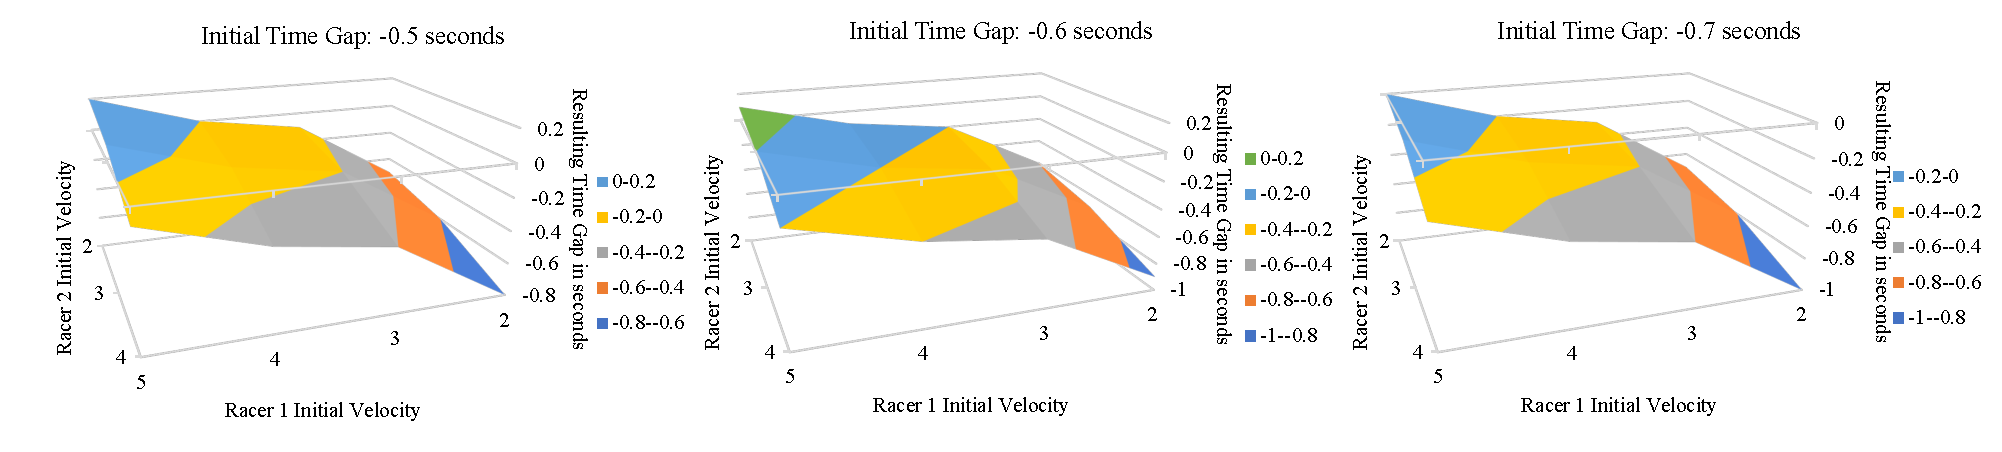
\includegraphics[width=\textwidth]{Figures/StraightExp.pdf}
    \caption[Results of scenarios in long straight case study.] { Plots for the resulting time gap by implementing both players' synthesized optimal strategy for various initial velocities and tire wear percentages in the long straight shape.}
    \label{fig:ls_exp}
\end{figure}

For each of the initial states we plot the resulting time gap assuming the players select their best action in Figure \ref{fig:ls_exp}. We observe a negative correlation between initial time disadvantage and the resulting time gap and a positive correlation between initial speed and the resulting time gap. Therefore, the results confirm that the model does meet the expected results based on the real-life understanding of where advantages are observed in this type of track shape. 
\begin{sidewaysfigure}
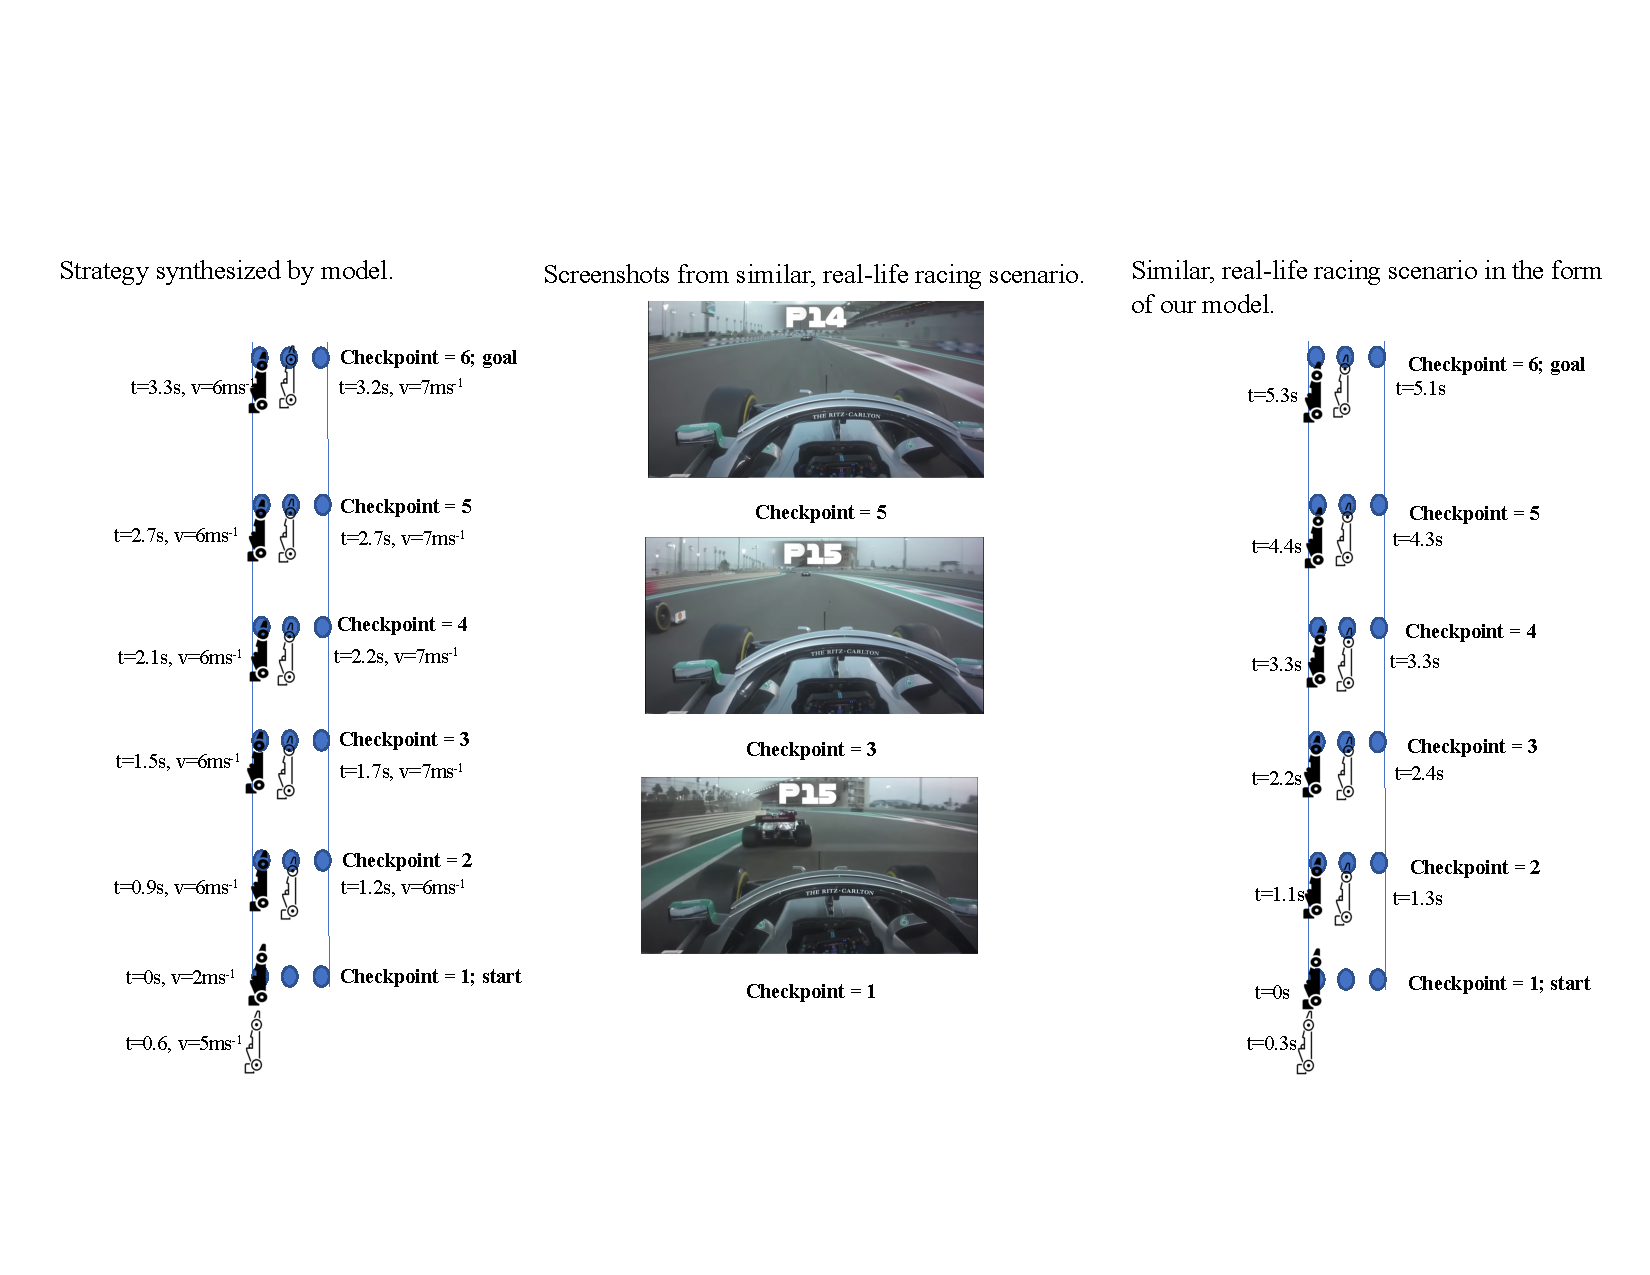
\includegraphics[height=0.8\textwidth, width=\textheight]{Figures/StraightViz.pdf}
    \caption[Synthesized strategy compared to real-life scenario on a long straight.] { Left: Visualized strategy synthesized in our case study scenario. Middle: Screenshots from a real-life race scenario resembling our case study.  Right: Extracted real race scenario represented in our model formulation.}
    \label{fig:ls}
\end{sidewaysfigure}
Next, we take a deeper dive in Figure \ref{fig:ls} by visualizing the players' strategies in one of the experiments. We show the specific scenario where the initial time disadvantage is \SI{0.6}{\second}, the initial velocity of racer 1 is \SI{5}{\meter\per\second} and the initial velocity of racer 2 is \SI{2}{\meter\per\second}. Player 1 and player 2 refer to the white car and black car, respectively. The synthesized strategy tells both cars to reach their top speeds, but it also indicates to player 1 to switch to the center lane. Player 1 is eventually able to build a \SI{0.1}{\second} time gap at the goal state due to its top speed advantage. The screenshots and the plotted real-life example\footnote{\label{straightnote}\url{https://youtu.be/z0tW3wY758Q?t=57}} is a straight section of the track that is about several hundred meters. While we don't know precise states of the players in the real-life video, we still use the video clip to plot the drivers' maneuvers using the time stamps. The tactic employed by the expert driver is similar to the one synthesized by the model in our case study. The driver switches to the center lane and uses the higher top speed and initial velocity to launch past the car that was originally in front. 

\FloatBarrier
% https://youtu.be/GxYzAqUs8N0?t=194
% https://youtu.be/64BQ-aXJkxA?t=28
% https://youtu.be/z0tW3wY758Q?t=57
\subsection{Hairpin}
 The second track shape is a hairpin turn, which is defined as a 180 degree turn. In reality, these types of turns generally follow long straights, but due state space explosion, the lead up to the hairpin turn is limited to just two checkpoints. Furthermore, because the turns are 180 degrees, the cars do not need to travel very fast. Therefore, having better acceleration and lower tire wear results in better performance in this type of track shape, and this pattern is seen in real-life races. In terms of strategy, the player that is initially ahead ideally positions itself in the middle of the straight approaching the turn to . Then, at the turn, the player wants to be at the innermost lane of the corner to force the opponent to take a wider turn or fall back in line. On the other hand, the player that is initially behind would like to reach the inside lane if at all possible and prevent the car that is ahead from using the inside lane. Tire wear begins to play an important role because it limits how tight of a turn is feasible for the players. Sometimes, the tire wear may be too high such that a player cannot use the inner most lane at the turn. Therefore, in the experiments for this scenario, we fix the initial time gap for racer 1 at 0.5 seconds but use varying combinations of initial velocities and tire wears for the racers. 

\begin{figure}[t!]
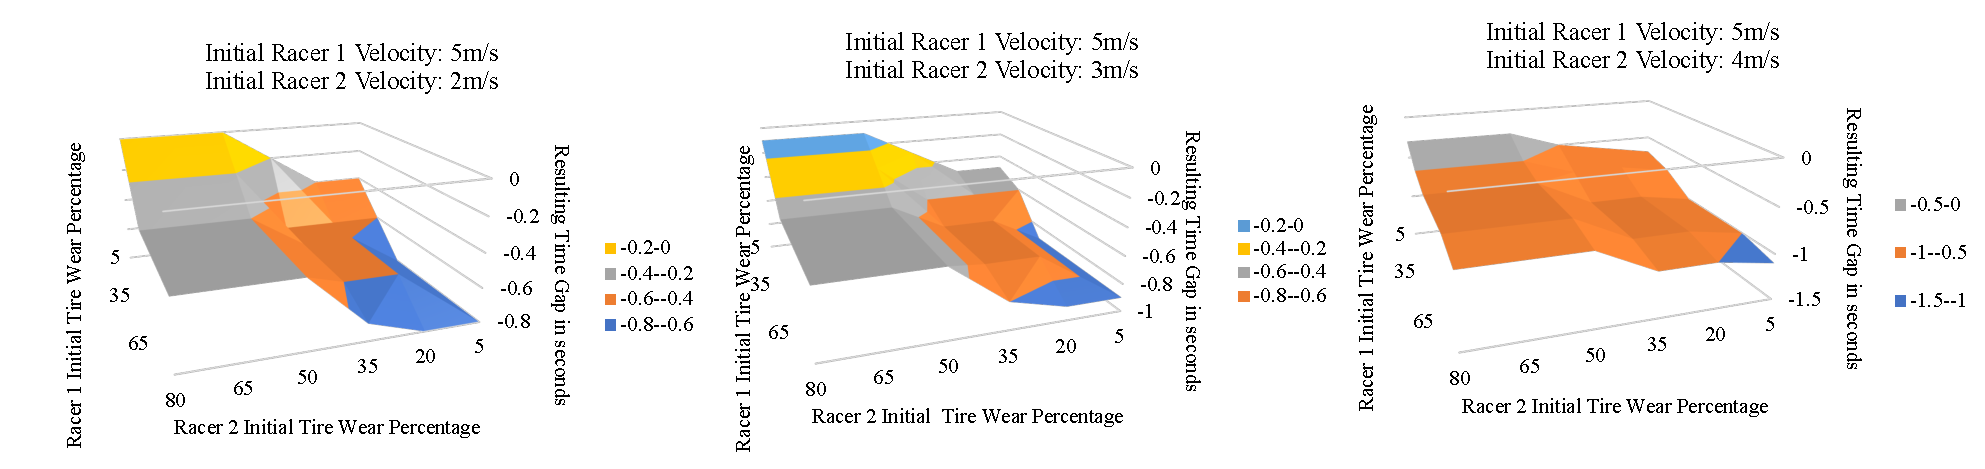
\includegraphics[width=\textwidth]{Figures/HairpinExp.pdf} 
    \caption[Results of scenarios in hairpin case study.] {Plots for the resulting time gap by implementing both players' synthesized optimal strategy for various initial velocities and tire wear percentages in the hairpin shape.}
    \label{fig:hp_exp}
\end{figure}

 In Figure \ref{fig:hp_exp}, we plot the results of our experiments. We see that player 2's higher acceleration allows it to stay ahead or only allow racer 1 to catch up but not pass despite having an initial velocity disadvantage. In other words, the player 1's time gap at the final checkpoint is always non-positive. The best case for player 1 is closing the time gap to 0 at the final checkpoint, and it occurs when player 2 is given a significant tire wear disadvantage. However, when there is a tire wear disadvantage for player 1, player 2 still maintained an advantage at the end despite having a lower initial velocity. These trends confirm that the model properly represents the advantages and disadvantages observed in real-life racing. 

\begin{sidewaysfigure}
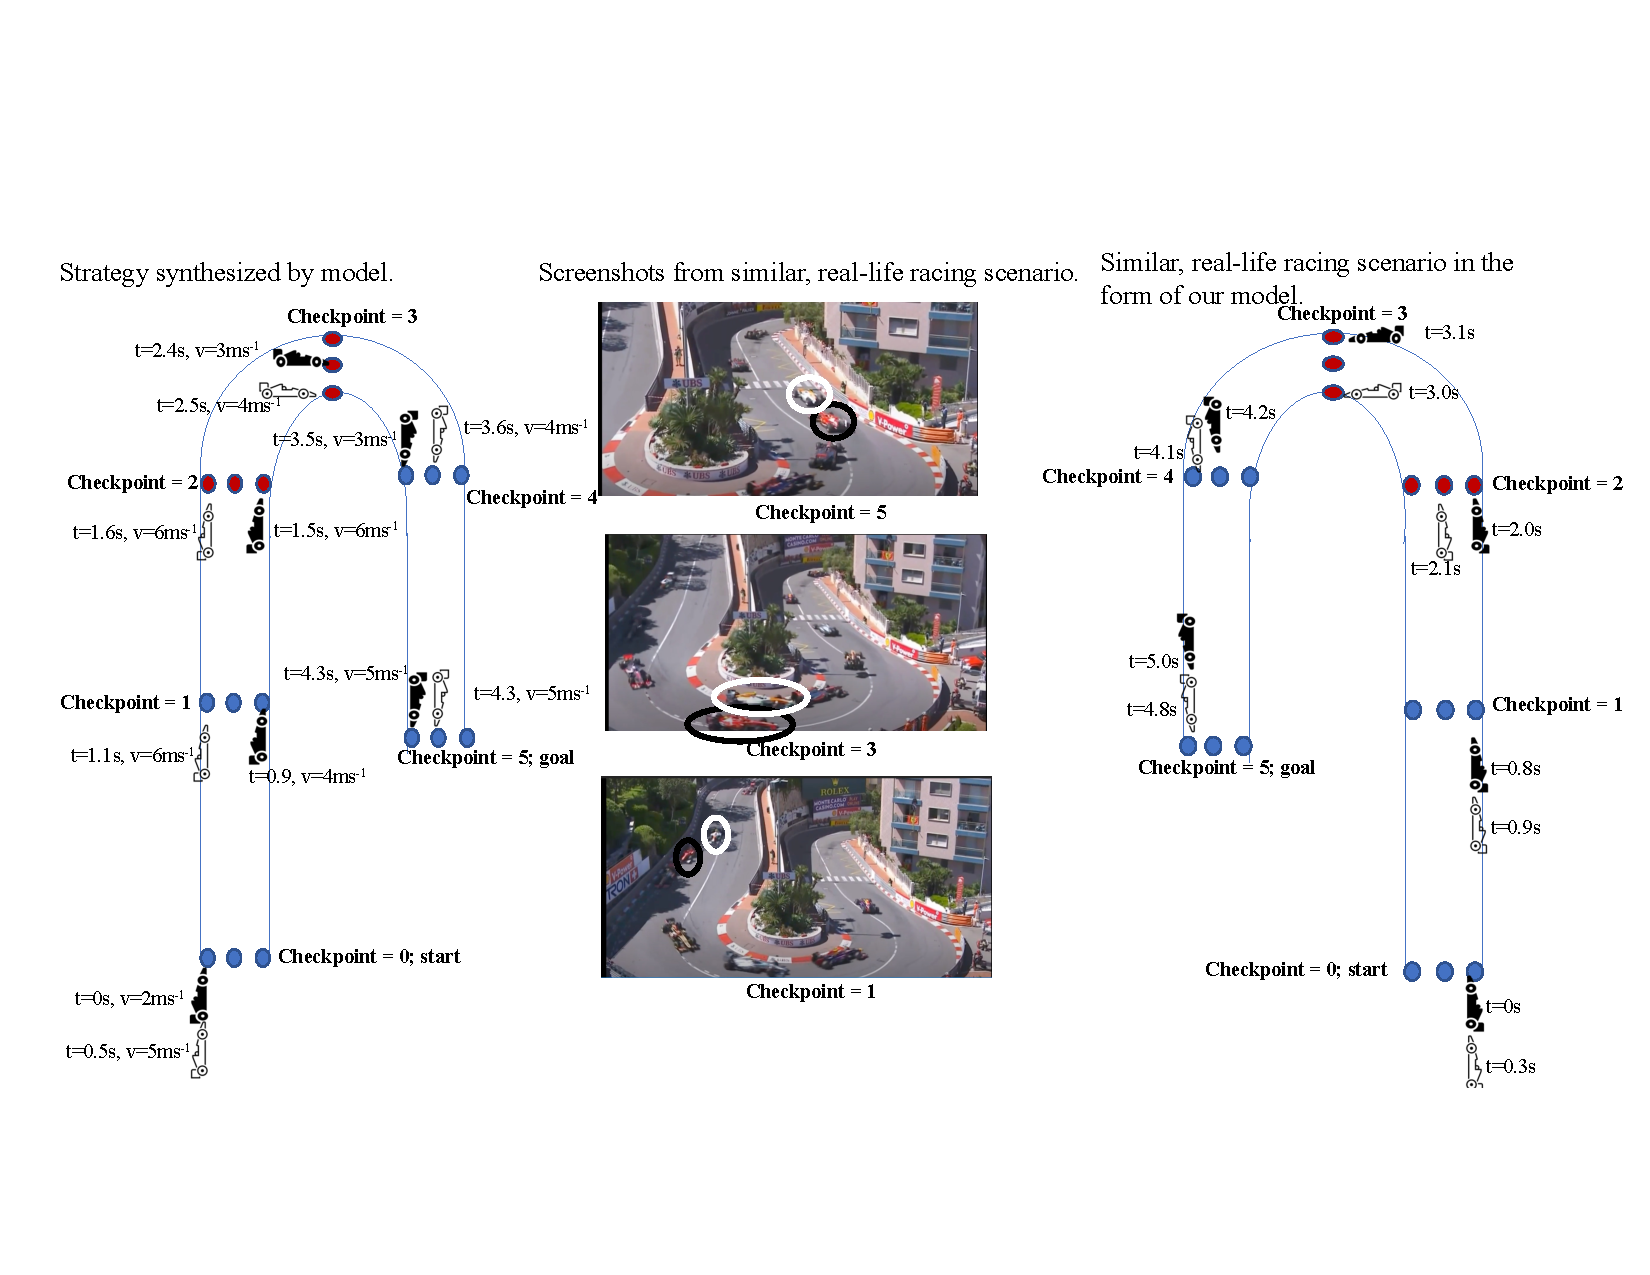
\includegraphics[height=0.8\textwidth, width=\textheight]{Figures/HairpinViz.pdf}
    \caption[Synthesized strategy compared to real-life scenario on a hairpin turn.] {Left: Visualized strategy synthesized in our case study scenario. Middle: Screenshots from a real F1 race.  Right: Extracted real race scenario represented in our model formulation.}
    \label{fig:hp}
\end{sidewaysfigure}

Next, we take a deeper dive in Figure \ref{fig:hp} to visualize the synthesized strategy from one of our scenarios. We study the scenario where player 1's initial velocity is 5 m/s, player 2's initial velocity is 2 m/s, player 1's initial tire age is 5\%, and player 2's initial tire age is 50\%. The screenshots from the real-life hairpin scenario\footnote{\label{hairpinnote}\url{https://youtu.be/CZdsBMhYnT4}} have other cars in the image, but the two main cars in question are circled in their respective colors matching the model extrapolation. Player 1 and player 2 refer to the white car and black car, respectively. In the synthesized model strategy, we see that player 2 immediately shifts over to the inner most lane to prevent any possible plan from the innermost lane because it knows that player 1 has both the tire age and speed advantage. However, player 2's state and dynamics prevent it from using the tightest lane in the turn due to its aged tires. As a result, it switches to the middle lane in the corner allowing player 1 to eventually choose the innermost lane. Upon the exiting the corner (from checkpoints 3 to 4), player 2 again chooses the inner most line because it is still ahead by \SI{0.1}{\second}. This choice forces player 1 use the wide lane and traverse a longer distance. As a result, player 1 is not able to overtake player 2, but it closes the gap to 0 seconds at the final position. This type of defensive maneuver of covering the inside lane, then going wide in the middle of the turn, and finally taking the inside on the exit of the turn is known as the ``switch-back'' in racing dialogue. The ``switch-back'' is commonly used by expert drivers because it sometimes catches the attacking driver off-guard. However, in the real-life video we compare to, we observe a slightly different strategy being executed. Player 1 passes player 2 because player 2 makes a sub-optimal choice and does not cover in the inside line at the hairpin. Rather, player 2 chooses to stay wide through out the turn allowing the fast approaching player 1 to take the inside lane at the corner and pass player 2 on the exit. 

% https://www.youtube.com/watch?v=CZdsBMhYnT4
\FloatBarrier
\subsection{Chicane}
 The final track shape is a chicane, which is a successive pair of turns of opposite direction (left-right or right-left). The chicane puts a greater emphasis on the tire wear than the prior two shapes, and success depends on the parameters of lateral force parameters of a player's vehicle. The inside of one turn is the outside of the following turn, so the racers must also have the low tire wear to maintain high speed over the shortest distance, which is hit the inside lane of both turns. Otherwise, compromising by selecting the middle lane may allow the other player to pass on the inside of one of the turns. In similar fashion to the hairpin case study experiments, we fix the initial time gap for player 1 at \SI{0.5}{\second} and use varying combinations of initial velocities and tire wears for these experiments.
 
 \begin{figure}[t!]
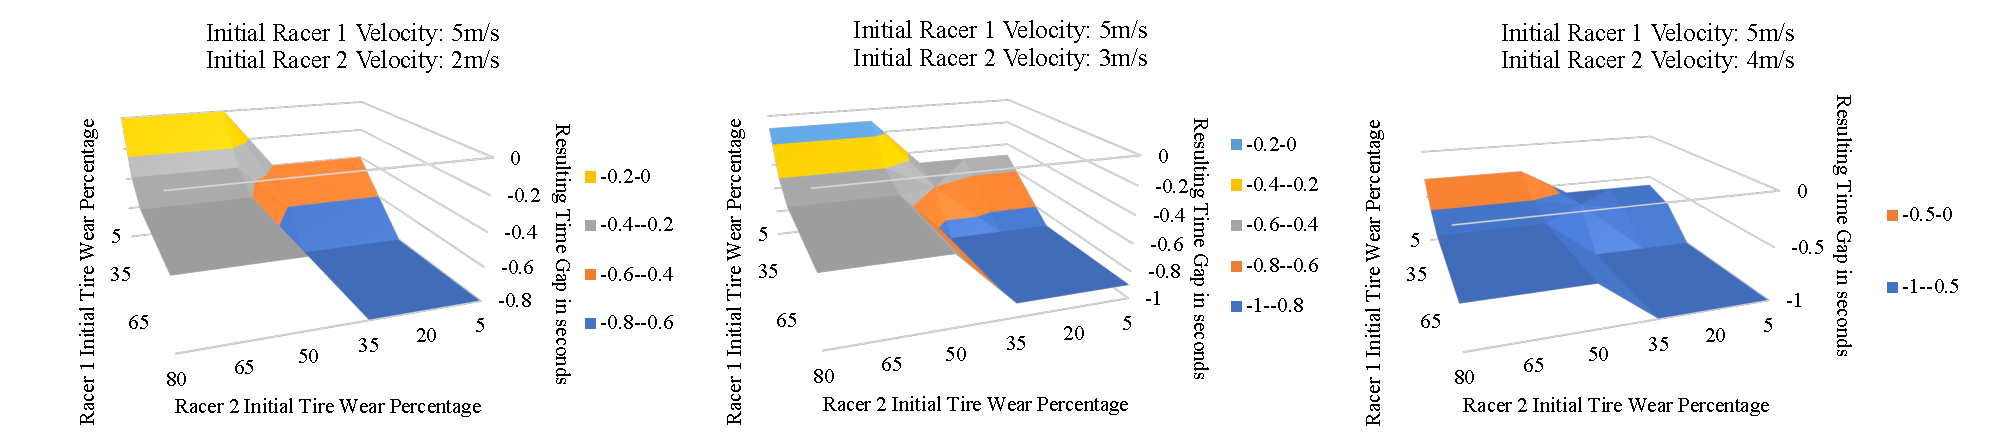
\includegraphics[width=\textwidth]{Figures/ChicaneExp.pdf}
    \caption[Results of scenarios in chicane case study.] {Plots for the resulting time gap by implementing both players' synthesized optimal strategy for various initial velocities and tire wear percentages in the chicane shape.}
    \label{fig:ch_exp}
\end{figure}
 
 Figure \ref{fig:ch_exp} shows a negative correlation between the final time gap between player 1 and player 2 and player 1's initial tire wear as expected. Furthermore, the lack of symmetry in surface of the plot shows the increased advantage for player 2 in some scenarios because it has a higher lateral acceleration limit. When the initial tire wear values are swapped for the racers, racer 2 maintains or builds on the initial \SI{0.5}{\second} time gap more often than racer 1 closes it. Again, the results indicate that model is a good representation of real-life racing because it follows the known patterns seen in real-life racing. 

\begin{sidewaysfigure}
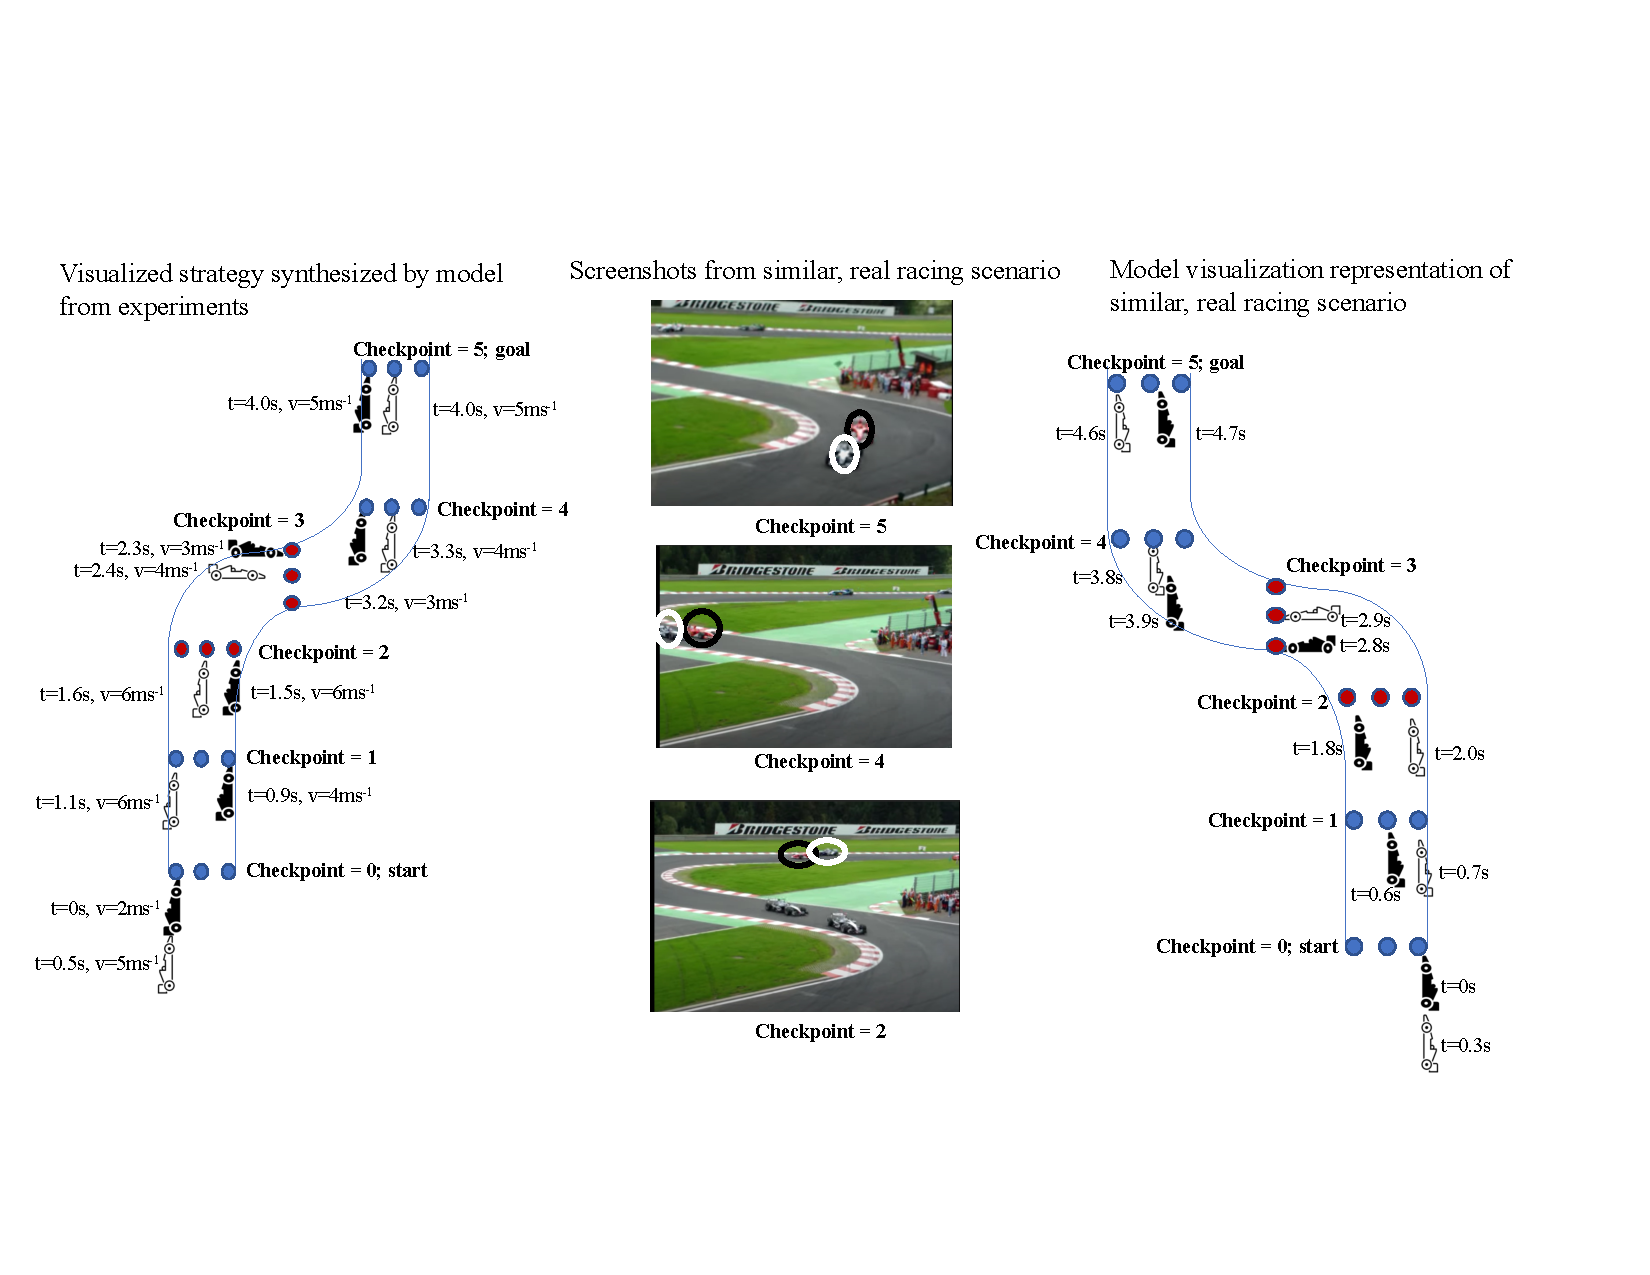
\includegraphics[height=0.8\textwidth, width=\textheight]{Figures/ChicaneViz.pdf}
    \caption[Synthesized strategy compared to real-life scenario on a chicane.]{Left: Visualized strategy synthesized in our case study scenario. Middle: Screenshots from a real F1 race. Right: Extracted real race scenario represented in our model formulation.}
    \label{fig:ch}
\end{sidewaysfigure}

In Figure \ref{fig:ch}, we visualize a synthesized strategy of one of the experiments over the chicane. We study the scenario where the the initial velocity of player 1 is \SI{5}{\meter\per\second}, the initial velocity of player 2 is \SI{2}{\meter\per\second}, the initial tire age of player 1 is 5\%, and the initial tire age of player 2 is 50\%. The screenshots from the real-life chicane scenario\footnote{\label{chicanenote}\url{https://youtu.be/_gWkHuOKR9w?t=6}} have the two main cars circled in their respective colors matching the model extrapolation. Player 1 and player 2 are the white and black cars, respectively. The synthesized strategy for this scenario presents a typical defensive maneuver where the initial leader, player 2, selects the inside line of both corners. This choice forces player 1 to use the wider line for both corners. However, player 1 has a lower tire wear and higher initial velocity, so he is able to improve the time gap and maintain a higher speed despite choosing the unfavorable line. As a result, initial time difference is reduced to \SI{0}{\second} at the final checkpoint. In the corresponding real-life scenario, we again observe a sub-optimal move by the leading human driver (in black) resulting in him being overtaken by the trailing driver (in white). The leading driver commits to the inside line for the first turn in the chicane, but stays wide on the second turn allowing the initially trailing driver to use the inside line at the second turn. As a result, the initially trailing driver has both the advantage of speed and shorter distance to travel with the inside line of the turn and makes the pass.  

\FloatBarrier
\section{Summary}
\begin{table}
\centering
\begin{tabular}{|l|l|p{4.5cm}|}
\hline
\textbf{Track Shape} & \textbf{Average Model Size} & \textbf{Average Time for Strategy Synthesis} 
\\ \hline
Straight   & 4200441 states      & \SI{394}{s}       \\ \hline
Hairpin   & 2139777  states     & \SI{200}{s}       \\ \hline
Chicane   & 2970922 states & \SI{273}{s}      \\ \hline
\end{tabular}%
\caption{Summary of model sizes and synthesis times for various track shapes.}
\label{table:discrete_exp_summary}
\end{table}
The results from the experiments show that our model provides a good representation of the prior understanding of advantage and disadvantage patterns in racing. We observe our discrete formulation and a state-of-the-art synthesis algorithm produce maneuvers that are comparable to those executed by professional human drivers while meeting the specification. In other words, the synthesized strategies follow all of the nuanced rules of racing while achieving the goal of reaching the target state before opponents or within the shortest time gap possible. In addition, we use these models to explain how the sub-optimal decisions of the human drivers in the real life-scenarios may have been corrected. The primary limitation of solving the discrete game formulation using formal methods is that it takes about 4 minutes, on average, to produce a result with various inputs we tested. Table \ref{table:discrete_exp_summary} summarizes the size of the game and average computation time. Therefore, we cannot directly use it for real-time control of an autonomous racecar suggesting we use probabilistic methods to approximate strategies.
\chapter{Hierarchical Control for Head-to-Head Racing} 
% \epigraph{\flushright The Turn}{}
\epigraph{\flushright The second act is called ``The~ Turn.'' The magician takes the ordinary something and makes it do something extraordinary.}{Christopher Priest, \textit{The Prestige}}
\label{chapter:hier}
\section{Hierarchical Control Design}
% \begin{figure}
%   \centering
%   \includegraphics[height=0.5\textheight]{Figures/ControlStructureVertical.png}
%   \caption{The continuous dynamic game (top) transformed into the high-level discrete game (middle). The discrete game solution created by the high-level planner (highlighted in green) is tracked by the low-level planner (bottom).}
%   \label{fig:overall_control}
% \end{figure}
\begin{figure*}
  \centering
%   \includegraphics[width=\textwidth]{Figures/FormulationBreakdown.png}
    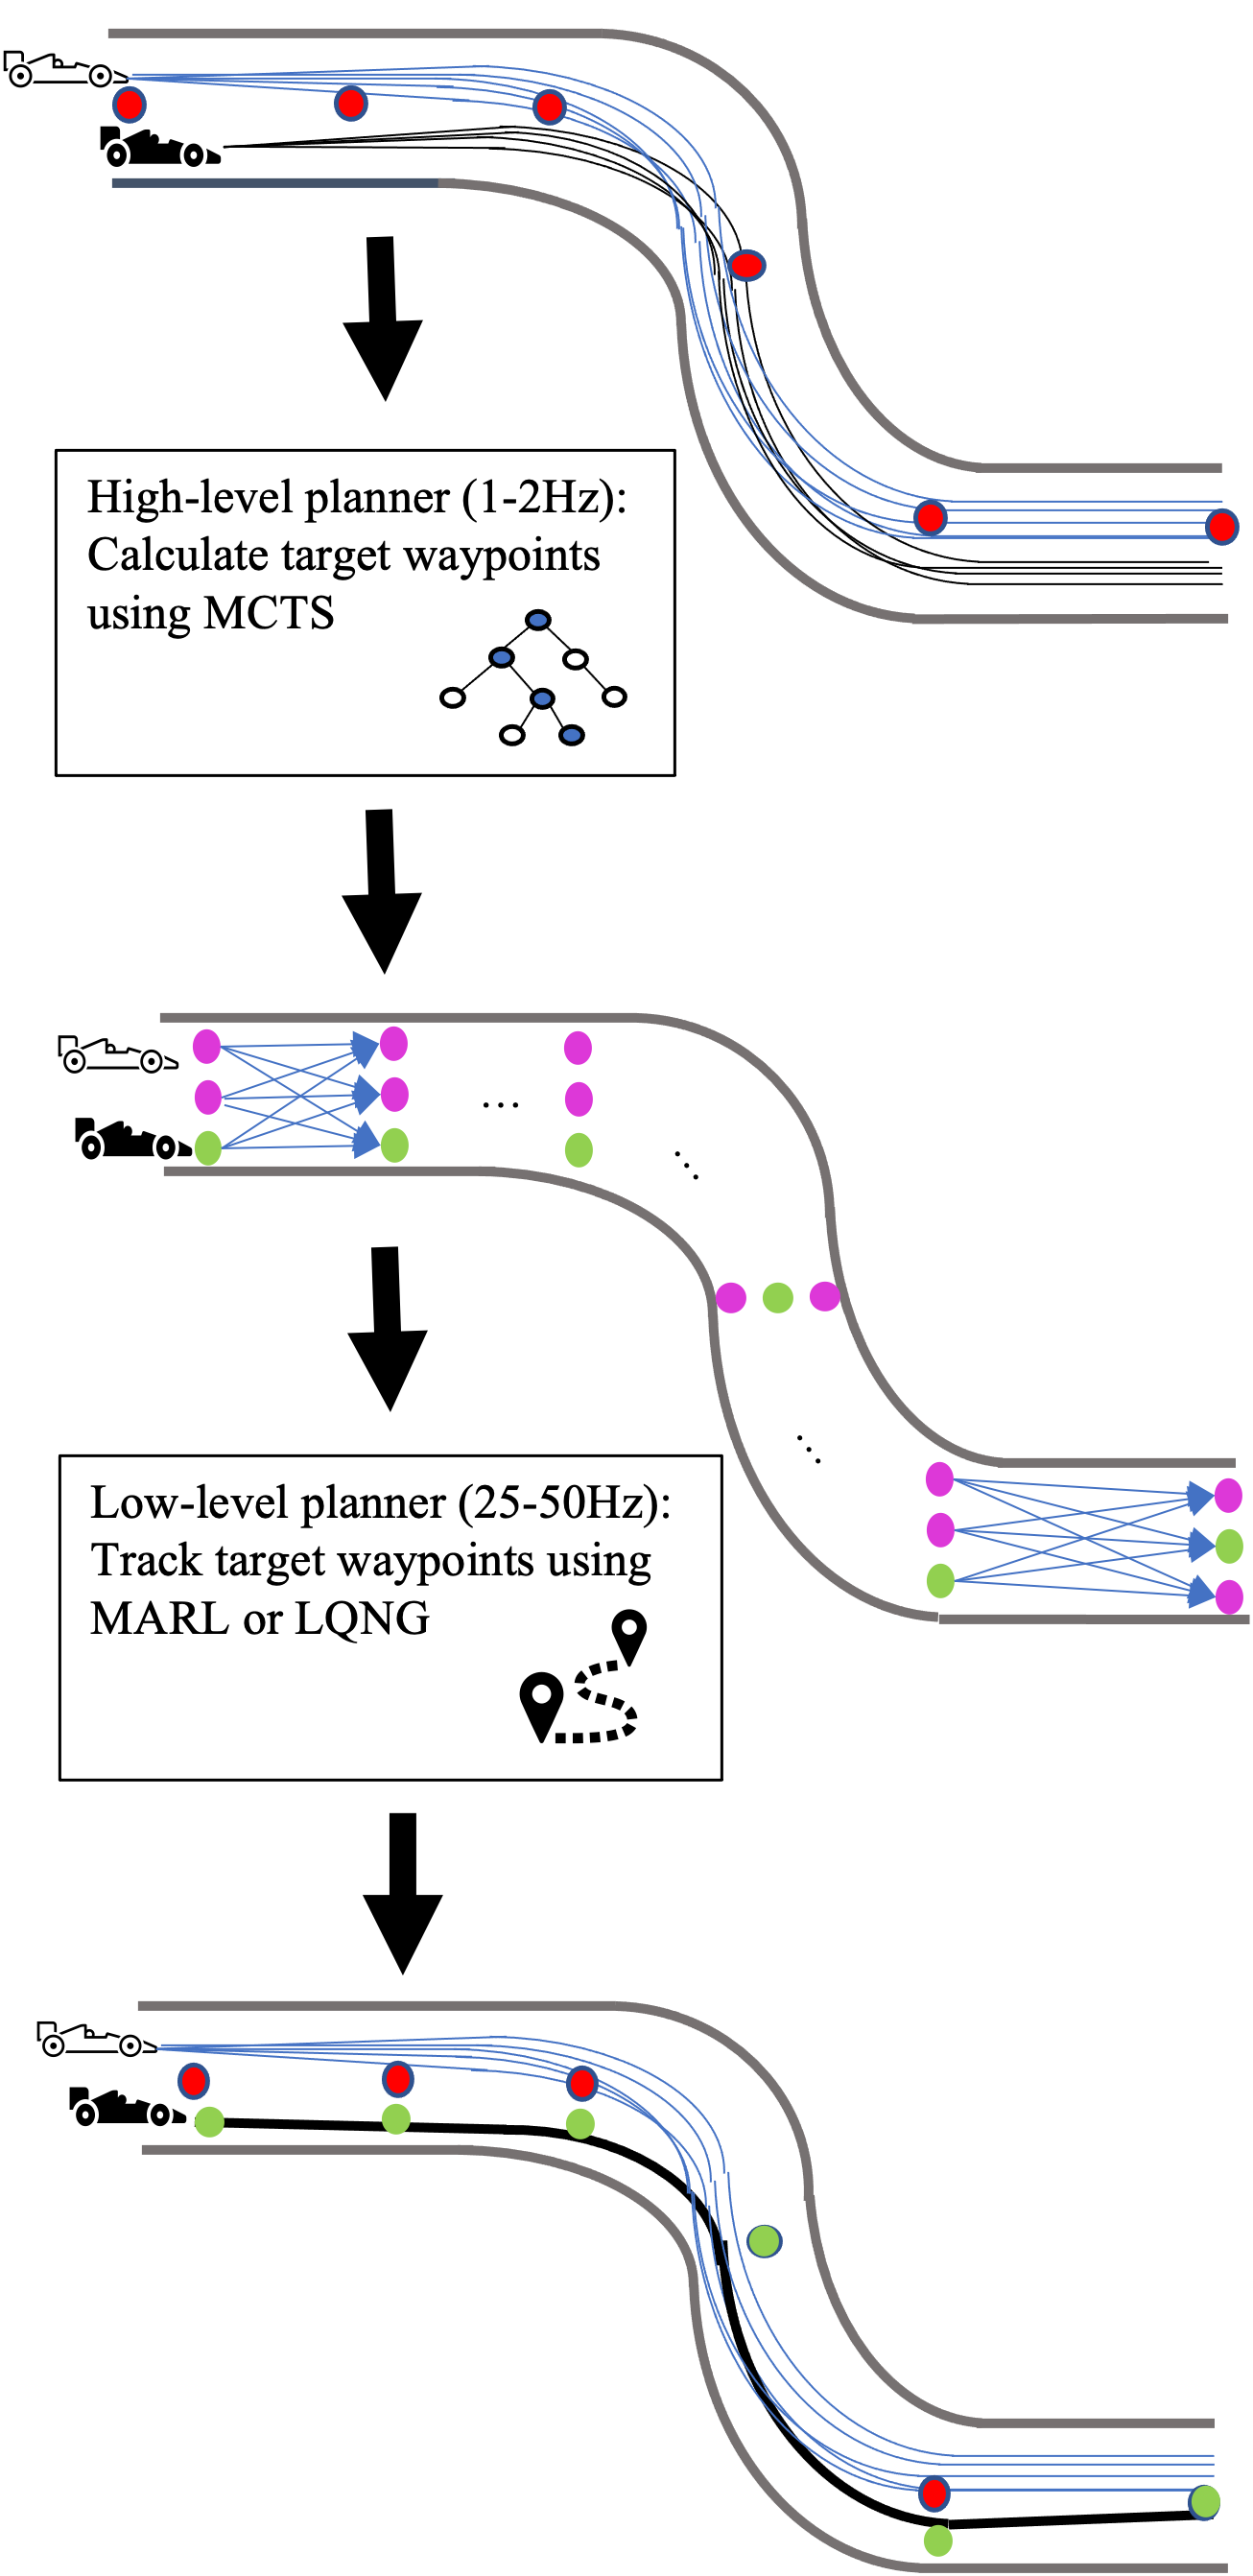
\includegraphics[height=0.8\textheight]{Figures/FormulationBreakdownVert.png}
  \caption[Hierarchical Control Architecture]{The uncountably infinite trajectories of the general game (top) discretized by the high-level planner (middle). The sequence of target waypoints calculated by the high-level planner (in green) is tracked by the low-level planner (bottom) and converges to a continuous trajectory (in black).}
  \label{fig:overall_control}
\end{figure*}
Traditional optimization-based control methods cannot easily be utilized for the general multi-agent racing game formulated with realistic safety and fairness rules in Section \ref{section:genform}. The rules involve nonlinear constraints over both continuous and discrete variables, and a mixed-integer non-linear programming algorithm would be unlikely to run at rates of \SI{25}{\hertz}-\SI{50}{\hertz} for precise control. This inherent challenge encourages utilizing a method such as deep reinforcement learning or trying to solve the game using short horizons. 

However, we propose a hierarchical control structure involving two parts that work to ensure all of the rules are followed while approximating choices that are optimal in the long term. The high-level planner constructs a discrete game approximation of the original formulation where all of the discrete rules are naturally encoded. The solution provided by the high-level planner is a series of discrete states (i.e waypoints) for each player, which satisfies all of the rules. Then, the low-level planner solves a simplified version of the racing game with an objective putting greater emphasis on tracking a series of waypoints and smaller emphasis on the original game-theoretic objective and a simplified version of the rules. Therefore, this simplified formulation can be solved by an optimization method at high control frequencies or be encoded in a neural network when using a learning-based method. 

This method assumes if the series of waypoints produced by the high-level planner is guaranteed to follow the rules, then the control inputs generated by the waypoint tracking low-level planner will also satisfy the rules of the original game when applied to the actual underlying system. Figure \ref{fig:overall_control} visualizes the overall control architecture. 

\subsection{High-Level Planner}
The high-level planner constructs a turn-based discrete, dynamic game that is an approximation of the general game outlined in Section \ref{section:genform}. We formulate the high-level game using the model developed in Section \ref{section:discgame} and solve it over a receding horizon of checkpoints near the player for real-time control. However, our choice of horizon extends much further into the future than an MPC-based continuous state/action space controller can handle in real time \cite{Wang2019}. In the following subsections, we briefly summarize how the discrete game constructed and how we use Monte Carlo tree search to approximately solve the game.

\subsubsection{Discrete Game Construction}
% Describe High-Level Game (states, transitions, rewards)
Constructing our discrete game relies primarily on forming the initial states of the players. Given the initial states, the remaining feasible states and transitions of the game arise naturally by following the dynamics in Section \ref{section:discdyn}. 

To select the initial state of the game, we first construct a subset of the overall set of players based on their distances from ego player. Because the discrete game is fixed to a finite horizon of checkpoints, the players that would likely have a significant impact on an ego player's trajectory are those who are within some local vicinity of the ego player. Using the set of local players, the initial checkpoint of the game is selected to be the one that the furthest forward player in the local vicinity has passed, and the target checkpoint is a fixed count ahead of that initial checkpoint. 

The continuous components of the players' states are projected into their discrete representations as described in Section \ref{section:discstate}. Initial state values for speed, velocity, tire wear, lane ID, and ``recent" lane changes are easily extracted from their continuous state. However, because some players may not have reached the selected initial checkpoint of the discrete game, their initial time state must be estimated. We assume every player has access to the times at which each checkpoint was passed by each of the other players. The initial time state is set to 0 for the furthest forward player. For each of the remaining players' initial time states is set based on the time difference between the furthest forward player and the player. Figure \ref{fig:disc_construct} shows this initial state construction process applied to a 4 player situation in the perspective of Player 1. Player 1 ignores Player 3 in the discrete game because he is out of the range of vicinity. Within Player 1's vicinity, Player 2 is the furthest forward player, so his time state in the discrete game is 0. Player 1 sets his time state as \SI{0.2}{\second} because the last passed checkpoint of both players was checkpoint 2, and the time difference at that checkpoint was \SI{0.2}{\second}. The same logic applies in setting Player 4's initial time state. The remaining state variables are categorized in the discrete buckets based on the player's state at whatever checkpoint they may be at. This simplification may be coarse, but in practice, a player's vicinity range is relatively small. Therefore, the state of the players' states do not change significantly within the range.

As mentioned, given the initial states of the players, the remaining construction of the game follows directly from the other parts of the formulation. The objective is the same as described in Section \ref{section:discobj}, but we do not use model checking software/algorithms to solve the game for our hierarchical controller. Table \ref{table:discrete_exp_summary} shows that it takes about 3-4 minutes to solve a single instance using state-of-the-art model checking software. We expect to run the high-level planner at \SI{1}{\hertz} to \SI{2}{\hertz}.

\begin{figure}
  \centering
%   \includegraphics[width=\textwidth]{Figures/FormulationBreakdown.png}
    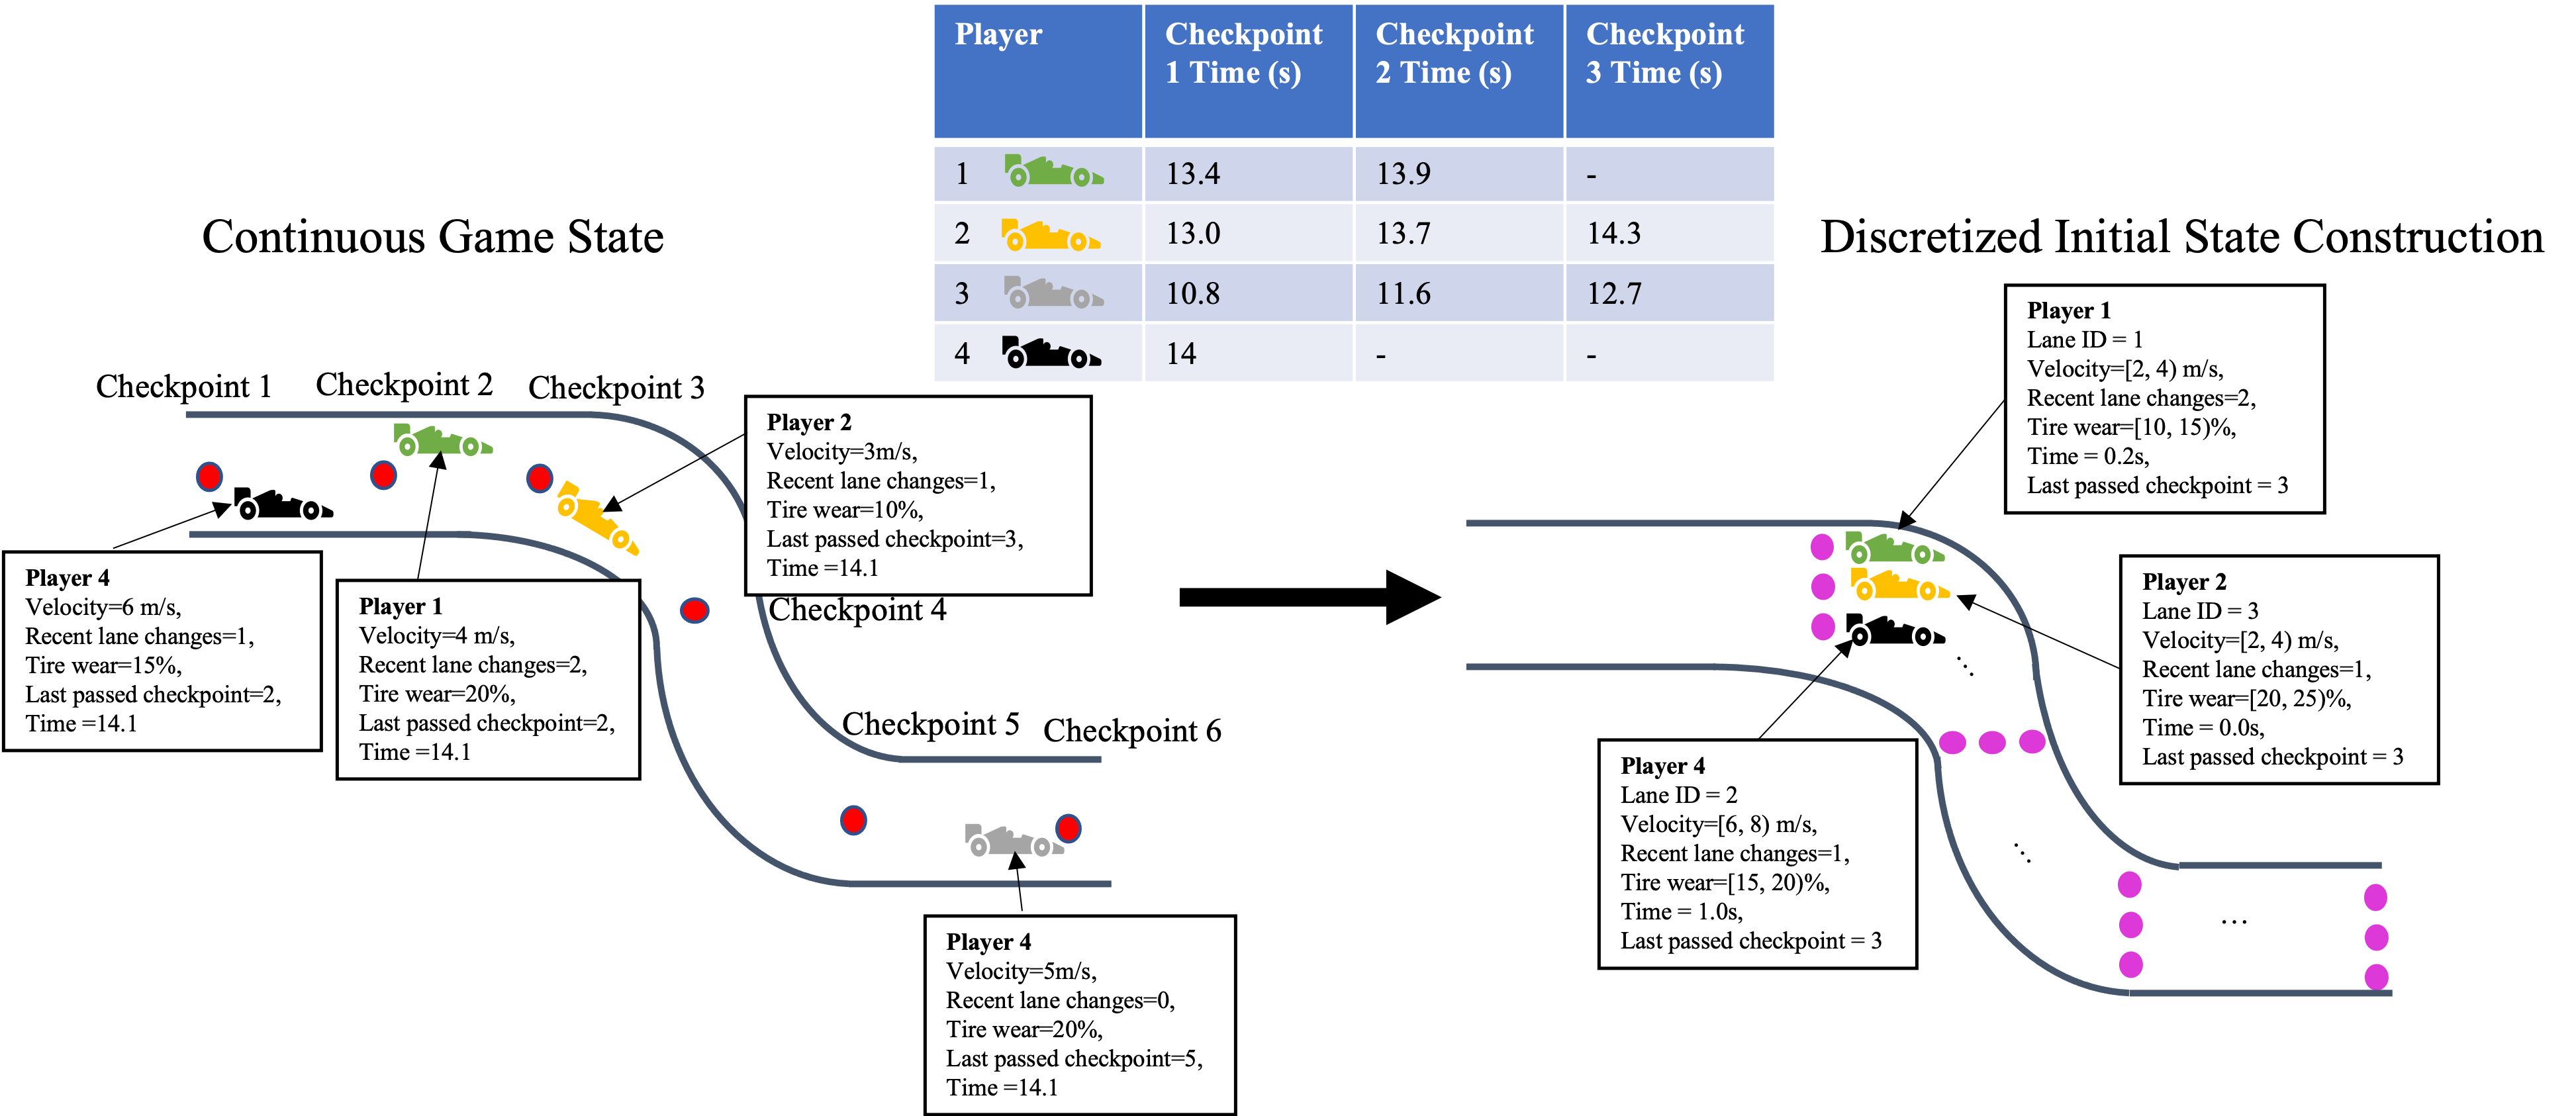
\includegraphics[width=\textwidth]{Figures/DiscreteInitialization.png}
  \caption[High-level planner discrete game initialization]{Using the checkpoint time table (top) and the continuous states (left), Player 1 constructs the initial state of the high-level discrete game (right).}
  \label{fig:disc_construct}
\end{figure}

\subsubsection{Monte Carlo Tree Search}
Although the discrete game is much simpler than the original formulation, its state space still grows exponentially as the number of actions and players increases. Therefore, we cannot rely on synthesizing strategies using model checking methods for real-time control. In order to produce a reasonable strategy for the discrete game in real-time, we use the Monte Carlo tree search (MCTS) algorithm to approximate the solution to our game \cite{mcts}. Our implementation of the MCTS algorithm is the same as the original with one exception: instead of sampling the feasible action set uniformly in the simulation step, we use a heuristic to bias our sampling towards those actions deemed more likely to be realistic or optimal. Recall that the actions available at each state is a set $A$ of pairs of lane ID and velocity. We sort the action set using following characteristics of each action in the following priority:
\begin{enumerate}
    \item Ascending by the elapsed time calculation \eqref{eq:time_update}
    \item Descending by target velocity of the action
    \item Ascending by absolute difference between target lane ID and current lane ID
    \item Ascending by the difference between target lane ID and the lane ID of the optimal racing line
\end{enumerate}
Once the actions are sorted, we randomly sample an index to select an action from the sorted set using following calculation:

\begin{equation}
    \text{action index} = [\min(|x|, |A|)], \quad
     x \sim \mathcal{N}(0, \frac{|A|}{6})
\end{equation}

Though the reward function is the same as the discrete formulation, we normalize it between 0 and 1 when calculating the upper confidence bound scoring in the MCTS algorithm. The solution produced by applying MCTS to our discrete game is a series of waypoints in the form of target lane IDs (which are mapped back to locations on track) and the target velocities at each of the locations. These waypoints are generated for all players considered in the discrete game and are selected assuming everyone selects their optimal choice. The top and middle of Figure \ref{fig:overall_control} visualize the original, continuous formulation expanded into a discrete space of lanes (in purple) and highlights target waypoints that might be calculated by MCTS (in green).  

\subsection{Low-Level Planner}
\subsubsection{Low-Level Simplified Game Formulation}
% Describe Simplified waypoint Following Game
The low-level planner is responsible for producing the control inputs, so it must operate at even higher frequencies than the high-level planner. Because we have a long-term plan in the form of target waypoints from the high-level planner, we formulate a reduced version of the original game for our low-level planner. The low-level game is formulated over a shorter horizon compared to the original game of just $\delta$ steps in $\hat{\mathcal{T}} = \{1, ..., \delta\}$. We assume that the low-level planner for player $i$ has received $k$ waypoints, $\psi^i_{r^i_{1}}, ..., \, \psi^i_{r^i_{1} + k}$, from the high-level planner. Lastly, we also refer to player $i$'s last passed checkpoint as $r^i_*$. 
% Table \ref{tab:ll_symbols} includes the additional parameters referenced in the simplified formulation.

The low-level objective involves two components. The first is to maximize the difference between its own checkpoint index and the opponents' checkpoint indices at the end of $\delta$ steps. The second is to minimize the tracking error, $\eta^i_y$, of every passed waypoint $\psi^i_{y}$. The former component influences the player to pass as many checkpoints as possible, which effectively pushes the player to reach $c_\tau$, the final checkpoint, as quickly as possible. The latter influences the player to be close to the high-level planner's target waypoints when passing each of the checkpoints. The objective also includes a multiplier $\alpha$ that balances the emphasis of the two parts. The objective is written as follows:
% Low-Level Formulation

\begin{equation} \label{eq:ll_obj}
    \min_{u^i_{1}, ..., u^i_{\delta}} (\sum^N_{j \neq i}r^j_{\delta} - (|N|-1) r^i_{\delta}) + \alpha \sum_{c={r^i_{1}}}^{{r^i_{1}}+k} \eta^i_c
\end{equation}

The players' continuous state dynamics, calculations for each checkpoint, and constraints on staying within track bounds  are effectively the same as the original formulation \eqref{eq:ll_dyn}-\eqref{eq:ll_pos_dist}. 

\begin{equation} \label{eq:ll_dyn}
    x^j_{t+1} = f(x^j_{t}, u^j_t), \quad \forall \;\; t \in \hat{\mathcal{T}}, j \in N
\end{equation}
\begin{equation} \label{eq::ll_pos}
    r^j_{t+1} = p(x^j_{t+1}, r^j_t), \quad \forall \;\; t \in \hat{\mathcal{T}}, j \in N
\end{equation}
\begin{equation} \label{eq::ll_pos_init}
    r^j_{1} = r^j_*, \quad \forall\;\; j \in N
\end{equation}
\begin{equation} \label{eq:ll_pos_dist}
    q(x^m_{t}) \leq w, \quad \forall \;\; t \in \hat{\mathcal{T}}, j \in N
\end{equation}

The collision avoidance rules are simplified to just maintaining a minimum distance $s_0$ as the high-level planner would have already considered the nuances of rear-end collision avoidance responsibilities defined in constraint \eqref{eq:gen_coll_avoid} from the general formulation. Therefore, we require the following constraint to hold for all $t \in \mathcal{T}$, $j \in N$, and $k \in N \setminus \{j\}$:
\begin{equation} \label{eq:ll_coll_avoid}
    d(x^j_{t}, x^k_t) \geq s_0
\end{equation}

Finally, we define the dynamics of the waypoint error, $\eta^i_y$, introduced in the objective. It is equivalent to the accumulated tracking error of each target waypoint $y$ that player $i$ has passed using a function $h: X\times X \rightarrow \mathbb{R}$ that measures the error accumulates the overall error when passing a waypoint. If a player has not passed a waypoint, then the variable indexed by that waypoint is set to 0. The variable's dynamics are expressed by the following constraint:

\begin{equation} \label{eq:ll_wp_err}
    \eta^i_y = \begin{cases} \sum_{t}^{\Hat{\mathcal{T}}} h(x^i_t, \psi^i_{c})  & \text{if } \exists \; r^i_t \geq y \\
    0 & \text{otherwise}
    \end{cases} 
    \quad \forall \; y \in \{r^i_{1}, ..., r^i_{1} + k\}
\end{equation}

% Low-Level params table
% \begin{table}[b]
% \centering
% \caption{Additional symbols in low-level formulation}
% \begin{tabular}{p{0.15\linewidth}|p{0.75\linewidth}}  \label{tab:ll_symbols}
% Symbol & Value  \\ 
% \hline
% $\hat{\mathcal{T}}$ & Set of steps in the game \\
% $\hat{\delta}$ & Shortened horizon \\
% $\alpha$      &   Weight parameter in objective emphasizing importance of hitting trajectory waypoints    \\
% $\psi^i_c$      &   Waypoint for player $i$ to target when passing checkpoint index $c$ \\
% $\eta^i_c$  &  Distance of player $i$'s closest approach to the waypoint $\psi^i_c$ \\ 
% $h(x^i_{t}, \psi^i_c)$  &  Function distance of player $i$'s state to waypoint $\psi^i_c$ \\  
% \end{tabular}
% \end{table}
% Describe Low-Level Formulation
This simplified formulation is similar to the general formulation. However, the constraints introduced by the complex fairness and safety rules are dropped since they are already considered by the high-level planner. The middle and bottom of Figure \ref{fig:overall_control} show how the target waypoints from the high-level planner (in green) are approximately tracked by a low-level planner to produce a continuous trajectory (in black). 

We consider two methods to solve this low-level formulation. The first method develops a reward and an observation structure to represent this simplified formulation for a multi-agent reinforcement learning (MARL) algorithm to train a policy that serves as a controller. The second method further simplifies the low-level formulation into a linear-quadratic Nash game (LQNG) to compute the control inputs. In the following subsections, we describe each of these low-level control methods.

\subsubsection{Multi-Agent Reinforcement Learning Controller}
% RL objective/reward structure for this game
Designing the MARL-based controller primarily involves shaping a reward structure that models the low-level formulation's objective and constraints. The RL agent is rewarded for the following behaviors that would improve the objective function \eqref{eq:ll_obj}:
\begin{itemize}
    \item Passing a checkpoint with an additional reward for being closer to the target lane and velocity.
    \item Minimizing the time between passing two checkpoints.
    \item Passing as many checkpoints in the limited time.
\end{itemize}
On the other hand, the agent is penalized for actions that would violate the constraints:
\begin{itemize}
    \item Swerving too frequently on straights \eqref{eq:gen_lane_lim}.
    \item Going off track or hitting a wall \eqref{eq:ll_pos_dist}.
    \item Colliding with other players \eqref{eq:ll_coll_avoid} with additional penalty if the agent is responsible for avoidance \eqref{eq:gen_coll_avoid}. 
\end{itemize}

The rewards capture our low-level formulation objective \eqref{eq:ll_obj} to pass as many checkpoints as possible while closely hitting the lane and velocity targets \eqref{eq:ll_wp_err}. The penalties capture the on-track \eqref{eq:ll_pos_dist} and collision avoidance \eqref{eq:ll_coll_avoid} constraints. Note that the penalties reintroduce the original safety and fairness from the original general game that were simplified away from the low-level formulation \eqref{eq:gen_coll_avoid} and \eqref{eq:gen_lane_lim}. Because these rules are inherently met by satisfying the objective of reaching the high-level planner's waypoints, their penalties have the weights set to have a lower impact than other components of the reward structure. We also justify incorporating the original form of these penalties because learning-based methods provide the freedom to easily encode these rules. Moreover, we are robustifying the low-level agent against the possibility that the ego player might be forced to deviate far away from the high-level plan in extreme circumstances.

The observation structure of the MARL controller captures the assumption of perfect information we have in all of our game formulations. Therefore, the observation structure consists of the following elements:
\begin{itemize}
    \item Perfect state information of one's own state and all other player states:
    \begin{itemize}
        \item Normalized velocity
        \item Lane ID
        \item Proportion of max allowed lane changes used
        \item Proportion of tire wear
        \item Proportion of checkpoints passed
        \item For opponent states only: 
        \begin{itemize}
            \item Position in the local coordinate frame
            \item Distance to opponent
        \end{itemize}
        \end{itemize}
    \item Local LIDAR distance observations spaced over a 180\textdegree{} field of view centered in the direction that the player is facing. Figure \ref{fig:lidar} displays the LIDAR rays captured by the MARL agents in our implementation.
    \item Locations and target velocities of upcoming $k$ waypoints, $\psi^i_{r^i_{1}}, ..., \, \psi^i_{r^i_{1} + k}$, in the local coordinate frame. 
\end{itemize}

\subsubsection{Linear-Quadratic Nash Game Controller}
% Linear approximation of the waypoint following game
Our second low-level approach solves an LQNG using the Coupled Riccati equations \cite{basar}. This method involves further simplifying the low-level formulation into a structure with a quadratic objective and linear dynamics. The continuous state is simplified to just four variables: $x$ position, $y$ position, $v$ velocity, and $\theta$ heading. The control inputs $u^i_t$ are also explicitly specified as acceleration, $a^i_t$, and yaw-rate, $e^i_t$. The planning horizon is reduced to $\Bar{\delta}$ where $\Bar{\delta} << \delta < T$. To construct our quadratic objective for player $i$, we break it into three components. The first is to minimize the distance to the upcoming target waypoint from the high-level planner $\Bar{\psi}^i$ calculated by the following equation:
\begin{multline} \label{eq:lqng_obj1}
\upsilon^i(\rho_1, \rho_2,\rho_3) =  \sum_{t = 1}^{\Bar{\delta}} (\rho_1((x^i_{t} - \Bar{\psi}^i_x)^2 + (y^i_{t} - \Bar{\psi}^i_y)^2) \\   \quad + \rho_2 (v^i_{t} - \Bar{\psi}^i_v)^2 
 + \rho_3 (\theta^i_{t} - \Bar{\psi}^i_\theta)^2)
\end{multline}

The second component is to maximize each opponent's distance from the location of his estimated upcoming target waypoint $\Bar{\psi^j}$. The opponent's target waypoint is estimated as his best response in the high-level MCTS game used plan player $i$'s target waypoints. However, recall that all opponents may not be considered in the MCTS planner if they were not in the vicinity when the high-level plan was computed. In that case, we assume $\Bar{\psi^j} = c_{r^j + 1}$, which is the opponent's upcoming checkpoint located at the center of the track. This component is calculated by the following equation:
\begin{equation} \label{eq:lqng_obj2}
    \phi^i(\Bar{\psi}^j, \rho) = \sum_{t = 1}^{\Bar{\delta}} \rho((x^j_{t} - \Bar{\psi}^j_x)^2 + (y^j_{t} - \Bar{\psi}^j_y)^2)
\end{equation}

We drop all of the constraints with the exception of collision avoidance, and it is incorporated as the third component and penalty term in the objective where the distance to each opponent should be maximized. This term is calculated by the following equation:
\begin{equation} \label{eq:lqng_obj3}
    \chi^i(x^j_t, y^j_t, \rho) = \sum_{t = 1}^{\Bar{\delta}} \rho((x^j_{t} - x^i_{t})^2 + (y^j_{t} - y^i_{t})^2)
\end{equation}

The final quadratic objective aggregates \eqref{eq:lqng_obj1}-\eqref{eq:lqng_obj3} using weight multipliers ($\rho_i$) to place varying emphasis on the components as follows:

\begin{equation} \label{eq:lqng_obj}
    \min_{a^i_{1}, e^i_{1}, ..., a^i_{\Bar{\delta}}, e^i_{\Bar{\delta}}}
    \upsilon^i(\rho_1, \rho_2,\rho_3)
    -\sum_{j \neq i}^{N}  (\phi^i(\Bar{\psi}^j, \rho_4) - \chi^i(x^j_t, y^j_t, \rho_5))
\end{equation}

Finally, the linear dynamics are time invariant and apply for all players $j \in N$:

\begin{multline} \label{eq:lqng_dyn}
\begin{bmatrix}
x^j_{t+1} \\
y^j_{t+1} \\
v^j_{t+1} \\
\theta^j_{t+1} \\
\end{bmatrix} = 
\begin{bmatrix} 
	1 & 0 & -\sin(\theta^j_{t_0})\Delta t & v^j_0\cos(\theta^j_{t_0})\Delta t\\
	0 & 1 & \cos(\theta^j_{t_0})\Delta t & v^j_0\sin(\theta^j_{t_0})\Delta t\\
	0 & 0 & 1 & 0\\
	0 & 0 & 0 & 1\\
	\end{bmatrix}
\begin{bmatrix}
x^j_{t} \\
y^j_{t} \\
v^j_{t} \\
\theta^m_{t} \\
\end{bmatrix}  +
\begin{bmatrix} 
	0 & 0 \\
	0 & 0 \\
	\Delta t & 0 \\
	0 & \Delta t \\
	\end{bmatrix}
	\begin{bmatrix} 
	a^j_t  \\
	e^j_t \\
	\end{bmatrix}
\end{multline}

\subsection{Summary of Control Structure}
Algorithm \ref{alg:control_loop} outlines the main control loop of the controller. The control loop is executed at a frequency greater than or equal to that of low-level planner. Because the rate of the high-level plan is lower than the rate of the main control loop, we just construct the initial game states and run the MCTS calculations on a background thread, asynchronously updating the target waypoints after the calculations are complete. For the low-level calculations, parallelism is not necessary because they are fast enough to meet the deadline of the main control loop. 

\begin{algorithm}
\caption{Control loop for hierarchical controller for a player $i$.}\label{alg:control_loop}
\begin{algorithmic}
\State $x^1,\ldots, x^{|N|} \gets \text{Current states of all players}$
\State $f_h \gets \text{High-level control frequency}$
\State $f_l \gets \text{Low-level control frequency}$
\State $t \gets \text{Elapsed time}$
\If{$r^i \neq c_\tau$} \Comment{Only run until we reach final checkpoint.}
\If{$t \mod 1/f_l = 0$} \Comment{Low-level control loop}
    \If{MARL Planner}
    \State $o \gets$ \Call{CollectObservations}{$x^1,\ldots, x^{|N|}$}
    \State $u^i_t \gets$ \Call{ComputeActions}{$o$}
    \ElsIf{LQNG Planner}
    \State $\Bar{\psi}^1,\ldots,\Bar{\psi}^{|N|}  \gets \psi^i_{r^i_{1}},\ldots,\psi^{|N|}_{r^{|N|}_{1}}$ 
    
    \Comment{Latest estimate of upcoming waypoint of each player.}
    
    \State $u^i_t \gets$ \Call{SolveLQNG}{$\Bar{\psi}^1,\ldots,\Bar{\psi}^{|N|}$}
    \EndIf
\EndIf
\If{$t \mod 1/f_h = 0$} \Comment{High-level control loop}
    \State $\Tilde{N} \gets$ \Call{$\text{NearbyPlayers}^i$}{$x^1,\ldots, x^{|N|}$}
    \State $\Tilde{x^1},\ldots, \Tilde{x^{|\Tilde{N}|}} \gets$ \Call{DiscreteProjection}{$\Tilde{N}$}
    \State $\psi^i_{r^i_{1}}, ..., \, \psi^i_{r^i_{1} + k} \gets$ \Call{MCTS}{$\Tilde{x^1},\ldots, \Tilde{x^{|\Tilde{N}|}}, \text{time limit}=1/f_h$} 
    
    \Comment{Run MCTS in background thread and save target waypoints.}
\EndIf
\EndIf
\end{algorithmic}
\end{algorithm}

The high-level planner is paired with each of the two low-level planners to produce two hierarchical controllers. We refer to our two hierarchical variants as MCTS-RL and MCTS-LQNG.

\section{Experimental Setup}
\subsection{Baseline Agents}
To measure the importance of our design innovations, we also consider three baseline controllers that resemble common planning and control methods developed in prior works.  
\subsubsection{End-to-End Multi-Agent Reinforcement Learning}
The end-to-end MARL controller, referred to as ``E2E," represents the pure learning-based methods such as those developed by Wurman et al. and Schwarting et al. \cite{sonyai, Schwarting2021}. This controller has a similar reward/penalty structure as our low-level controller, but its observation structure is slightly different. Instead of observing the sequence of upcoming states as calculated by a high-level planner, E2E only receives the subsequence of locations from $\{c_i\}_{i=1}^{\tau}$ that denote the checkpoints at center of the track near the agent. As a result, it is fully up to its neural networks to learn how to plan strategic and safe moves. 

\subsubsection{Fixed Trajectory Linear-Quadratic Nash Game}
The fixed trajectory LQNG controller, referred to as ``Fixed-LQNG," uses the same LQNG low-level planner as our hierarchical variant, but it instead tracks a fixed trajectory around the track. This fixed trajectory is a racing line that is computed offline for a specific track using its geometry and parameters of the vehicle similar to prior works by Vazquez et al. and Stahl et al. \cite{Vazquez2020, Stahl2019_2}. However, the online tracking involves game-theoretic reasoning rather than single-agent optimal control in the prior works.

\subsubsection{Fixed Trajectory Multi-Agent Reinforcement Learning}
The fixed trajectory MARL controller, referred to as ``Fixed-RL," is a learning-based counterpart to Fixed-LQNG. Control inputs are computed using a deep RL policy trained to track the precomputed target waypoints fixed prior to the race.  
\subsection{Controller Implementation}
% Implemented in Unity, used ML-Agents library for RL training
Our controllers are implemented\footnote{\codeurl} in the Unity Game Engine. Screenshots of the simulation environment are shown in Figure \ref{fig:experiment_tracks}. We extend the Karting Microgame template provided by Unity \cite{microkarting} to model our vehicles and racing environments. 

The kart physics from the template utilize Unity's built-in Rigidbody physics engine by simply updating the kart's velocity and yaw-rate at each control step using the acceleration and steering angle as inputs. However, to incorporate cornering limitations and tire wear modeling we modify the calculations. Tire wear proportion $e$ is modeled as an exponential decay curve that is a function of the accumulated angular velocity endured by the kart. This model captures the concept of losing grip as the tire is subjected to increased lateral loads. 

The velocity update of the kart is clamped between 0 and $\min(v_*, v_{\text{max}})$ where $v_{\text{max}}$ is the kart's maximum allowed top speed from the fixed parameters of the kart and $v_*$ is the maximum allowed velocity based on the kart's evolved state and turning radius. The calculation for $v_*$ is used in Section \ref{section:discdyn} of the discrete game formulation to approximate feasibility of certain actions depending on the shape of the track. It is calculated by first linearly interpolating the minimum lateral acceleration $a_{\text{max}}$ and maximum lateral acceleration $a_{\text{max}}$ by the proportion of tire wear $e$ to compute the maximum allowed lateral acceleration for the kart $a_*$. Then $a_*$ is used with turning radius of the vehicle $r$ and standard formulas of circular motion to compute $v_*$. The calculations are summarized by the following pair of equations:
\begin{equation}
     a_* = a_{\text{max}} - (a_{\text{max}}-a_{\text{min}})e
\end{equation}
\begin{equation}
    v_* = \sqrt{a_*r}
\end{equation}

Multi-agent support is also added to the template in order to race the various autonomous controllers against each other or human players. The high-level planners run at \SI{1}{\hertz}, and low-level planners run at \SI{13}{\hertz}-\SI{50}{\hertz}. $\Bar{\delta}$, the planning horizon for the LQNG planner, is set to \SI{0.06}{\second} for all controllers using it. The implementation of the learning-based agents utilizes a library called Unity ML-Agents \cite{mlagents}. All of the learning-based control agents are trained using proximal policy optimization and self-play implementations from the library. They are also only trained on two sizes of oval-shaped tracks with the same number of training steps. 


\begin{figure}
  \centering
  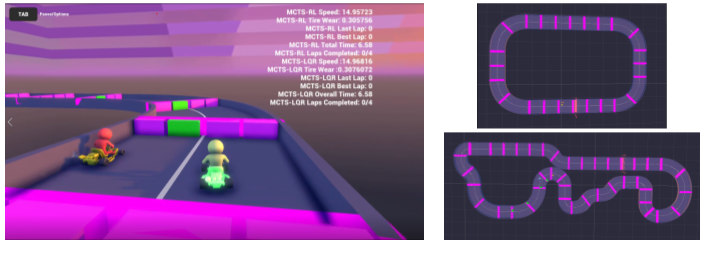
\includegraphics[width=\textwidth]{Figures/UnityEnvironment.png}
  \caption[Screenshots of Unity simulation environment] {Kart racing environment from a racer's perspective (left), a bird's eye view of the oval track (right-top), and the complex track (right-bottom) in the Unity environment. The purple boxes visualize the lanes across checkpoints along the track, and the highlighted green boxes show planned waypoints determined by the hierarchical controllers.}
  \label{fig:experiment_tracks}
\end{figure}
\section{Head-to-Head Racing Results}
% Two Tracks, 50 races head to head each
Our experiments include head-to-head racing on a basic oval track (which the learning-based agents were trained on) and a more complex track shown in Figure \ref{fig:experiment_tracks}. Specifically, the complex track involves challenging track geometry with turns whose radii change along the curve, tight U-turns, and turns in both directions. To be successful, the optimal racing strategy requires some understanding of the shape of the track along a sequence of multiple turns. Every pair of controllers competes head-to-head in 50 races on both tracks. The dynamical parameters (cornering limitations, top speed, acceleration, braking, etc.) of each player's vehicle are identical, and the players start every race at the same initial checkpoint with the same initial tire wear of 20\%. The only difference in their initial states is the lane in which they start. In order to maintain fairness with respect to starting closer to the optimal racing line, we alternate the starting lanes between each race for the players.

Our experiments primarily seek to identify the importance of hierarchical game-theoretic reasoning and the strength of MCTS as a high-level planner for racing games. We count the number of wins against each opponent, average collisions-at-fault per race, average illegal lane changes per race, and a safety score (a sum of the prior two metrics) for the controllers. Appendix \ref{app:hier_results} provides a complete breakdown of all of the head-to-head results. We also provide a video\footnote{\vidurl} demonstrating our controllers in action. 

\begin{table}
    \centering
    \begin{tabular}{|p{4cm}|l|l|}
    \hline
        \textbf{Aggregate Results (400 Total Races)} & \textbf{Wins} & \textbf{Average Safety Score} \\ \hline
        MCTS-RL & 333 & 0.91 \\ \hline
        E2E & 201 & 1.98 \\ \hline
        Fixed-RL & 238 & 0.93  \\ \hline
        MCTS-LQR & 119 & 1.89 \\ \hline
        Fixed-LQR & 97 & 0.79 \\ \hline
    \end{tabular}
    \caption[Aggregated head-to-head racing results.]{Aggregated head-to-head racing results across both tracks.}
    \label{tab:aggr_results}
\end{table}

\begin{figure}
  \centering
  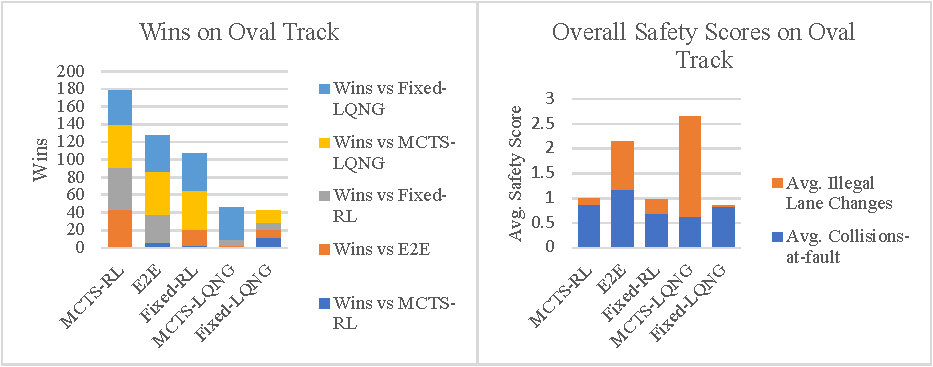
\includegraphics[width=\textwidth]{Figures/HeadOvalResults.pdf}
  \caption{Results from head-to-head racing on the oval track.}
  \label{fig:results_oval}
\end{figure}

\begin{figure}
\centering
  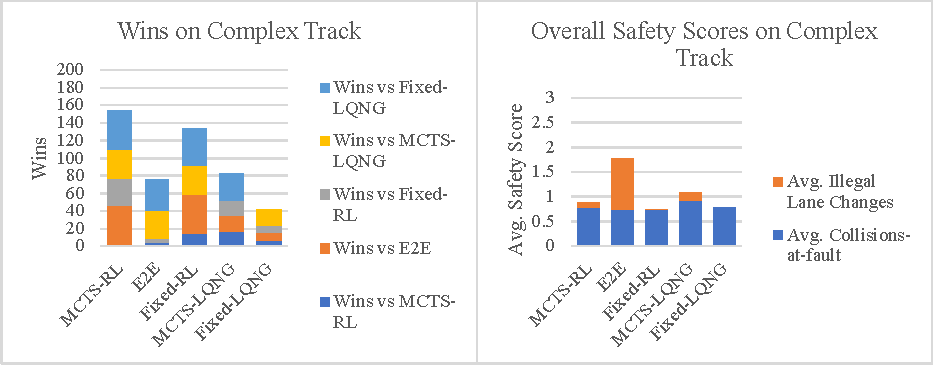
\includegraphics[width=\textwidth]{Figures/HeadComplexResults.pdf}
  \caption{Results from head-to-head racing on the complex track.}
  \label{fig:results_complex}
\end{figure}
\FloatBarrier
Based on the plots in Figure \ref{fig:results_oval} and Figure \ref{fig:results_complex} and Table \ref{tab:aggr_results}, we conclude the following key points:

\begin{enumerate}[wide, labelindent=0pt, font=\bfseries]
% MCTS-based variants outperformed respective baselines
\item \textbf{The proposed hierarchical variants outperformed their respective baselines.} 

The results amongst MCTS-RL, Fixed-RL, and E2E show the effectiveness of our hierarchical structure. While all three of the MARL-based agents were only trained on the oval track, the MCTS-RL agent won the most head-to-head races by compared to two baselines despite being trained with the same environment. Furtheromore, MCTS-RL's safety score is significantly better than E2E's safety score and practically the same as Fixed-RL's safety score. Comparing the baselines against each other, Fixed-RL also has more wins than E2E aggregated across both tracks. This result indicates that some type of hierarchical structure is favorable. It suggests that a straightforward task of trajectory tracking is easier to learn and more effectively generalized for a deep neural network than having to learn both strategic planning and respect for the safety and fairness rules. Specifically, while learning collision avoidance was reasonably captured by all of the MARL-based agents, E2E struggled with learning the illegal lane changes rule. On the other hand, the hierarchical structured agents did not have to focus on learning such a complex rule because they rely on a provided trajectory that is assumed to follow the lane changing rules.

Next, we compare MCTS-LQNG and Fixed-LQNG. Although MCTS-LQNG has a worse overall safety score, it has 25\% more wins when aggregated over both tracks. Furthermore, the main difference in their safety score is attributed to the fact that MCTS-LQNG considers multiple trajectories whereas Fixed-LQNG only follows a fixed trajectory that does not involve changing lanes often. Therefore, it is rare for Fixed-LQNG to break the lane changing rule. When just comparing their collision-at-fault counts, they are similar. Although on the oval track Fixed-LQNG has more wins against the MARL-based agents, when the racetrack gets more complicated, Fixed-LQNG quickly becomes inferior. The oval track has just one main racing line. However, there are many feasible racing lines in the complex track to consider in order to be competitive. MCTS-LQNG accounts for these trajectories by using the high-level MCTS planner and is therefore more successful in its races against MARL-based agents on the complex track with twice as many wins against them compared to the Fixed-LQNG agent. MCTS-LQNG considered trajectories that could result in overtakes when opponents made mistakes from any part of the track. On the other hand, Fixed-LQNG was forced to rely on opponents making mistakes that were not along its fixed trajectory to make overtakes. 

% RL is better than LQNG for low-level
\item \textbf{MARL is more successful and robust than LQNG as a low-level planner.}  

Overall, the MARL-based agents outperformed their LQNG-based counterparts in terms of both key metrics: wins and safety scores. However, this result is likely due to the heuristic simplifications in our LQNG design. Vehicle dynamics are only linearized around the initial state of each agent and are time-invariant, meaning the linear approximation is only valid for a very short time horizon. Therefore, the LQNG-based agents could only rely on braking/acceleration instead of yaw-rate to avoid collisions. As a result, the weights in the objective of the LQNG formulation are set conservatively to emphasize avoiding collisions. This setup also implies that LQNG-based agents often concede in close battles and thereby lose races because of the high cost in the planning objective of driving near another player even if there is no collision. Due to these properties, most of their races were decided over the first few turns of the race. If the LQNG-based agent was able to find itself ahead after the first several turns, then it usually built a considerable lead, especially Fixed-LQNG, that its opponents could not catch because the controller is very effective at tracking any trajectory with no obstacles. However, more often, it would fall behind or collide with an opponent at the start of the races causing it to lose speed. Once it fell behind, it could catch up to its opponents, but it could not successfully overtake unless the opponents made significant mistakes allowing it to pass with a considerable safety margin. If the dynamics were linearized over the state at each timestep $t$ instead of just the initial state at $t_0$, we could use a larger time horizon and expect better performance for the LQNG-based agent. 

While Fixed-RL and Fixed-LQNG have similar safety scores, MCTS-RL has a significantly better safety score than MCTS-LQNG. This difference primarily arises from increased illegal lane changes by the LQNG-based counterpart. The high-level planner runs in parallel with the low-level and at a lower frequency. As a result, the calculated high-level plan is sometimes delayed and does not account that the low-level controllers have already made choices that might contradict the initial steps in the plan. This mismatch causes the LQNG-based controller to more often break the lane changing rules by swerving across the track to immediately follow the high-level plan when it is updated. The MARL-based agents are more robust to this situation because they have those safety rules encoded in their reward structures, albeit with smaller weights. 

% MCTS-RL is the best overall controller.
\item \textbf{MCTS-RL outperforms all other implemented controllers.}  

 Aggregating the results from both tracks, MCTS-RL recorded a win rate of 83\% of the 400 head-to-head and the second best safety score behind the conservatively tuned Fixed-LQNG agent. It combined the advantage of having a high-level planner that evaluates long-term plans and a low-level planner that is robust to the possibility that the high-level plans may be out of date. For example, Figure~ \ref{fig:mctsrl:overtake} demonstrates how the high-level planner provided a long-term strategy, guiding the agent to give up an advantage at present for a greater advantage in the future when overtaking. The RL-based low-level planner approximately follows the high-level strategy in case stochasticity of the MCTS algorithm yields a waypoint that seems out of place (e.g., the checkpoint between $t=3$ and $t=4$ in Figure~ \ref{fig:mctsrl:overtake}). Furthermore, MCTS-RL is also successful at executing defensive maneuvers as seen in Figure~ \ref{fig:mctsrl:defense} due to those same properties of long-term planning and low-level robustness. Both of these tactics resemble strategies of expert human drivers in real head-to-head racing.
 \end{enumerate}
 
 \begin{figure}
    \centering
  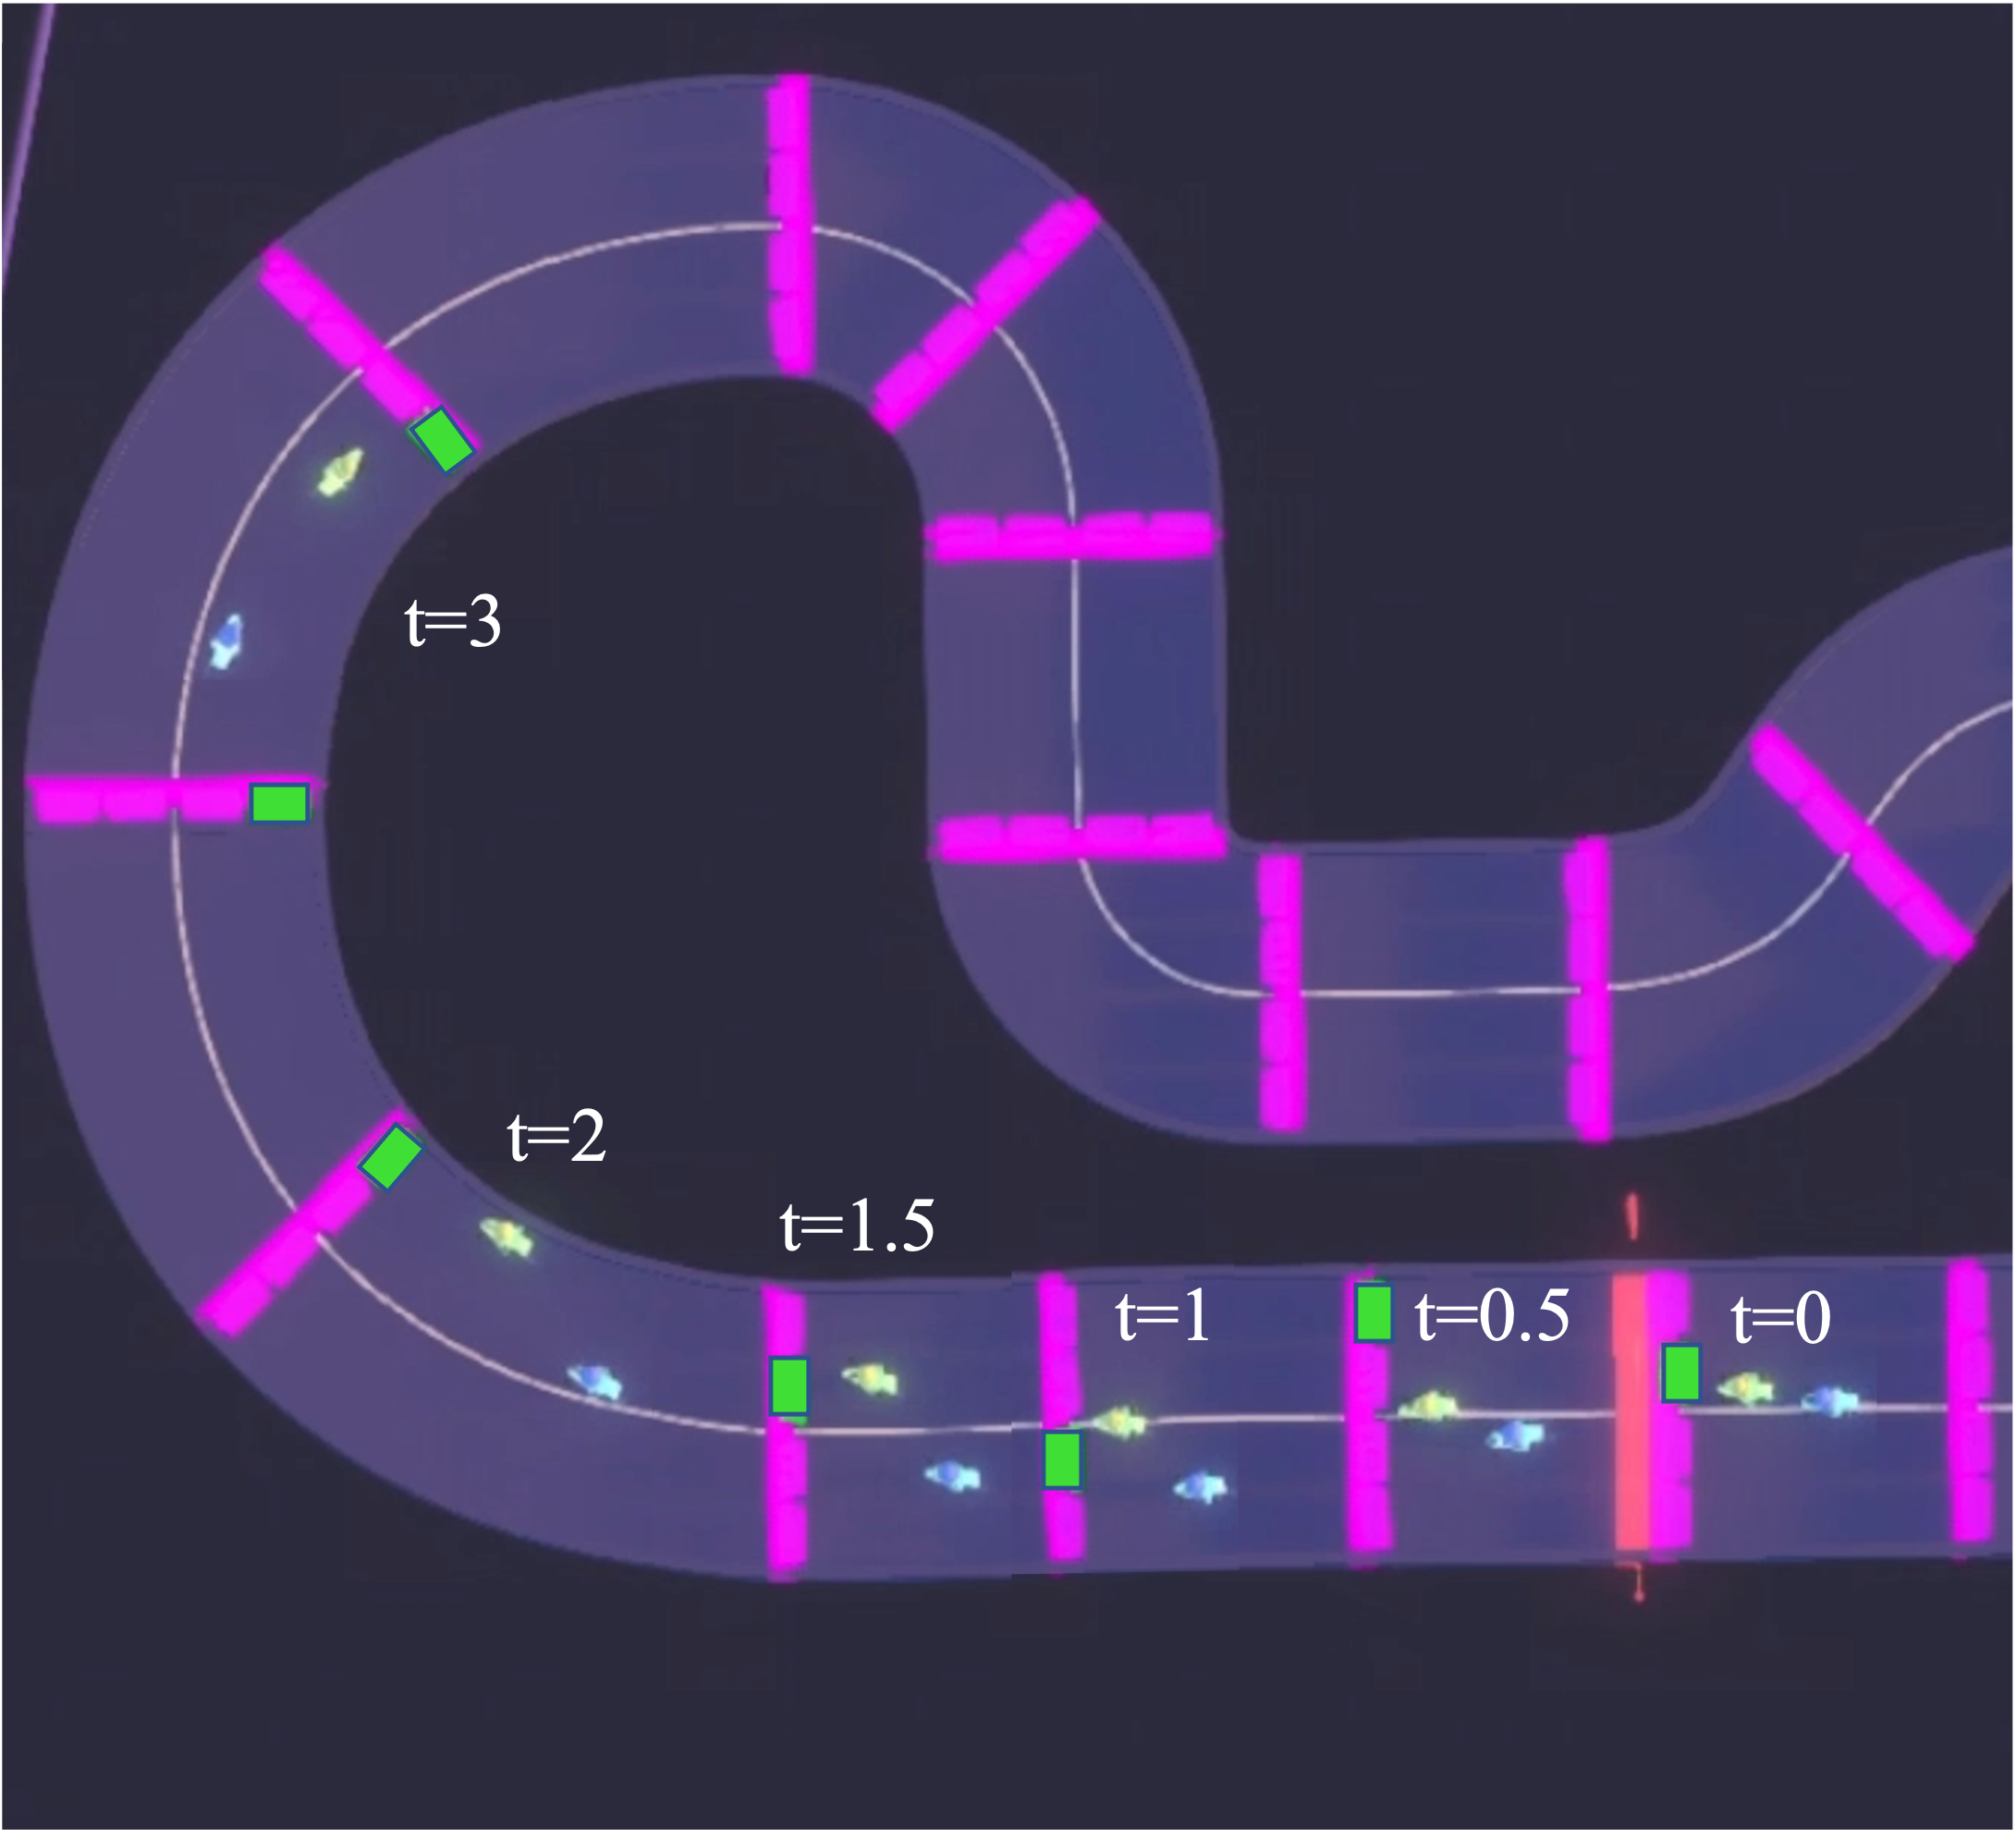
\includegraphics[width=0.7\textwidth]{Figures/MCTSRLDefense.png}
  \caption[Defensive maneuver by MCTS-RL controller.]{A defensive maneuver executed by the MCTS-RL agent (green) against the E2E agent (blue) on the complex track.  Before reaching the turn, the MCTS planner calculates to switch lanes to the left first ($t=0$ to $t=1$) and then move to the right for the inside of the turn. This motion forces the E2E agent to make an evading move to avoid collision and take an even wider turn, thus increasing the overall gap at the end. The green boxes along each checkpoint highlight the long-term plan calculated by the MCTS planner for this tactic.}
  \label{fig:mctsrl:defense}
\end{figure}

 \begin{sidewaysfigure}
  \centering
  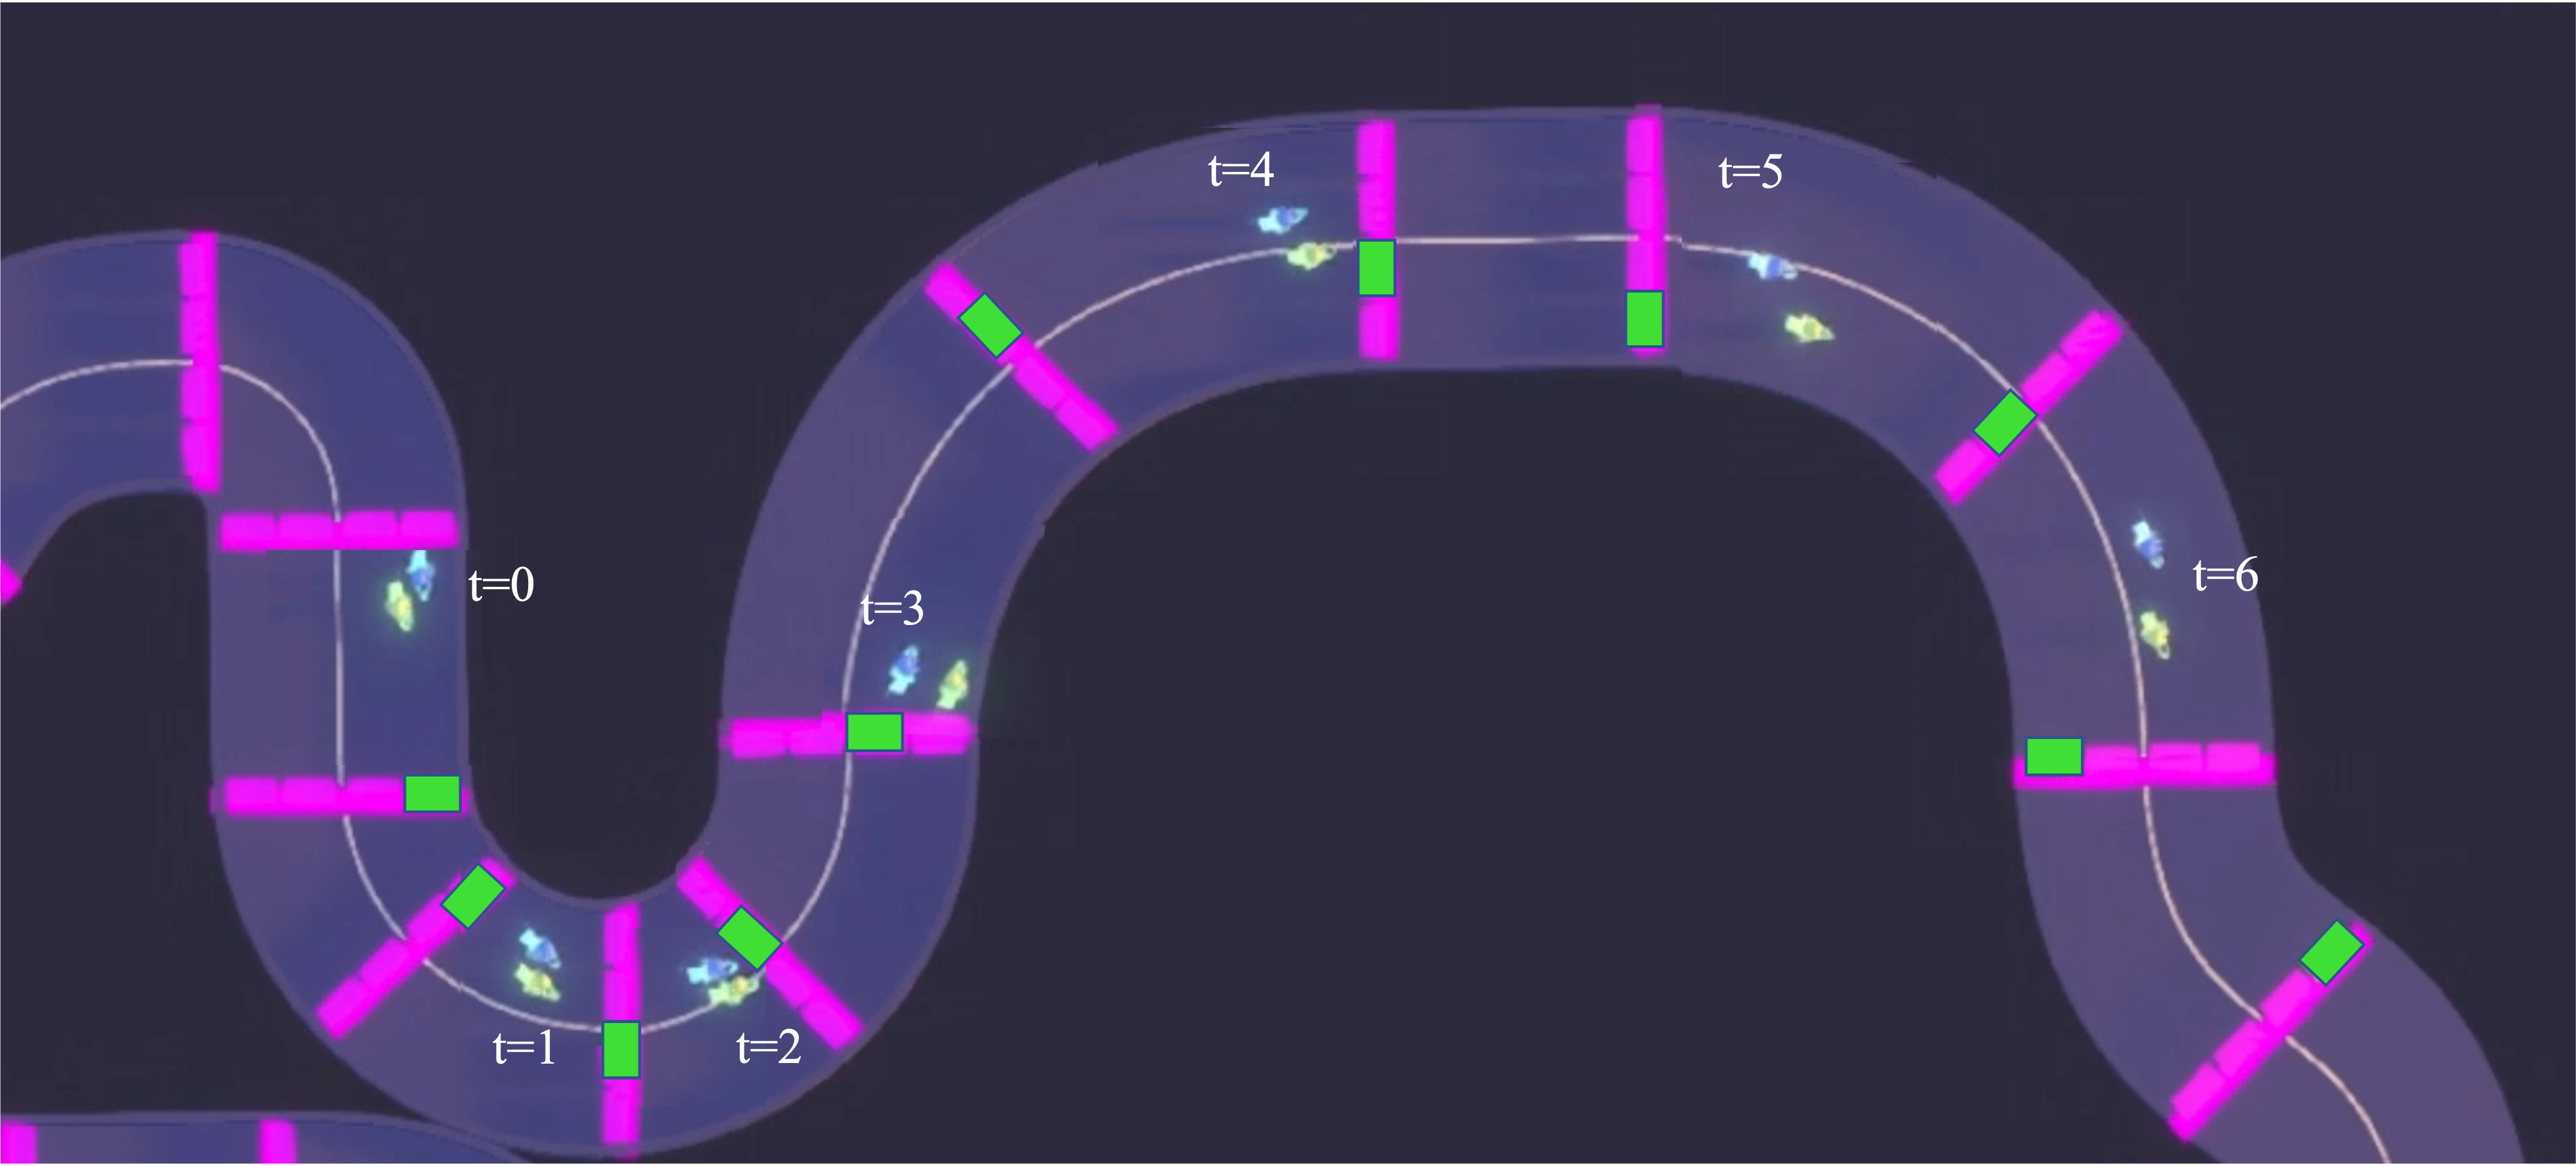
\includegraphics[width=\textwidth]{Figures/MCTSRLOvertake.png}
  \caption [Overtaking maneuver by MCTS-RL controller.] {An overtaking maneuver executed by the MCTS-RL agent (green) against the E2E agent (blue) on the complex track. Notice how, from $t=0$ to $t=2$, the MCTS-RL agent gives up a slight advantage and takes a wider racing line on the first turn. However, the exit of the wide racing line of the first turn places the MCTS-RL agent at the inside of the next two turns where it is able to gain an even greater advantage when passing the E2E agent from $t=3$ to $t=6$. The green boxes along each checkpoint also highlight the long-term plan calculated by the MCTS planner for this tactic.}
  \label{fig:mctsrl:overtake}
\end{sidewaysfigure}


\chapter{Hierarchical Control for Team-Based Multi-Agent Racing}
% \epigraph{\flushright The Prestige}{}
\epigraph{\flushright Because making something disappear isn't enough; you have to bring it back. That's why every magic trick has a third act, the hardest part, the part we call ``The Prestige."}{Christopher Priest}
\label{chapter:team}
The final part of this report introduces another important facet of real-life racing: teamwork. Most professional racing series such as IndyCar, Formula 1, and Formula E involve two competitions that run concurrently. There is an individual competition amongst the drivers, but there is also a competition over the overall performance of the racing teams based on the finishing positions of their drivers. Therefore, drivers are required to race with a mix of cooperative and competitive objectives in mind. 

Consider the example in Figure \ref{fig:team_motivating}. Player 1 and player 2 are on one team, and players 3 and 4 are on another team. Player 1 is clearly first and almost at the finish line, so it is unlikely that player 3, who is in second, can catch him before the finish line. On the other hand, player 4 is in last, but he is close to player 2 in third. Player 3 now has three high-level choices to consider:
\begin{enumerate}
    \item Try hard to overtake player 1 before the finish line.
    \item Maintain one's position to the finish line.
    \item Purposely slow down with the risk of being passed by player 2, but also improve the chances of player 4 overtaking player 2 by blocking player 4.
\end{enumerate}
If all players were on their own team, choice 1 would be the most obvious because that's where one would expect the maximum payoff. However, because there is an incentive to finish higher overall as a team, player 3 must consider the payoffs from all three choices. The payoffs and the risks associated with these choices are not necessarily obvious to evaluate. 

Incorporating such complexities only makes the the original problem harder to solve. Therefore, we propose that using our hierarchical control structure developed over the prior two chapters would allow players to evaluate the long-term implications of complex strategies in team-based autonomous racing while still adhering to the rules of the game. 

\section{Team-based General Racing Game Formulation}

\section{Team-based Hierarchical Control}
\subsection{Team-based High-Level Discrete Game Formulation}
\subsection{Team-based Low-Level Formulation}
\section{Team-based Racing Results}
\chapter{Conclusion} \label{chapter:conclusion}
Autonomous racing serves as a compelling application to develop control algorithms because it involves scenarios with complex rules and objectives. We construct a hierarchical game-theoretic controller for autonomous racing by breaking the challenging problem into two simplified levels. The high-level component encodes the complex rules, which often include constraints over discrete parameters and variables, by constructing a discrete abstraction of the game. Using a discrete representation allows us to consider maneuvers deeper in the future and simplifies the problem for our low-level controller, which just needs to follow the provided long-term plan. We show that hierarchical game-theoretic reasoning produces behavior that is not only competitive but also safer with respect to the rules. 

Abstractly, hierarchical reasoning represents how we, as humans, make long-term decisions when taking on a challenging task. It is impossible to consider all of the details and implications for every situation along the way to complete the task. Therefore, we break the problem into a sequence of discrete checkpoints that we consider reaching along the way to achieving our final goal. 

\section{Summary of Contributions}
This report introduces the following key contributions:
\begin{enumerate}
    \item We develop a model to transform a complex head-to-head racing game with realistic safety and fairness rules into a simplified discrete game with temporal logic specifications. This representation is solved by model checking tools to produce strategies that resemble those performed by human experts.
    
    \item We use our discrete game model as a high-level planner and combine it with a pair of low-level controllers using multi-agent reinforcement learning and linear-quadratic Nash game methods to produce a pair of hierarchical controllers. The discrete model is solved in real-time using Monte Carlo tree search to estimate a strategic plan that is tracked by the low-level controllers. Our hierarchical controllers outperform other baseline controllers resembling prior works in autonomous racing research. The hierarchical structure enables them to produce and execute plans that are optimal in the long-term and mirror those seen in real-life racing.
    
    \item We extend our hierarchical control design to a team-based racing game where players have a mix of competitive and cooperative objectives. To our knowledge, this report is the first work to study this problem. We show that our hierarchical controller scales to the even more complex problem and outperforms the baseline methods adapted to the team-based racing game. Again, our model produces behavior that mimics strategies executed by expert human drivers.
\end{enumerate}
\section{Future Extensions}
Future extensions of this work should introduce additional high-level and low-level planners. Examples of additional low-level controllers include time-varying linear-quadratic approximations or iterative best response methods. With a larger collection of control options, one might investigate policy-switching hierarchical controllers where we switch between various high and low-level controllers depending on the state of the game. For example, we noticed in our experiments that the LQNG-based controllers are reliable in situations where there are no nearby opponents avoiding any risk of issues arising from using a black-box MARL-based controller. Furthermore, if there are no other players nearby, then the high-level control can also switch to following the fixed, optimal line as all other racing trajectories would be sub-optimal. Deciding when to make such switches would possibly require an additional layer of hierarchy.

Lastly, our hierarchical control design can be extended to other multi-agent systems applications where there exist complex rules such as energy grid systems or air traffic control. Constructing a discrete high-level game allows for natural encoding of the complex constraints, often involving discrete components, to find an approximate solution that can warm start a more precise low-level planner.

\appendices
% \renewcommand{\thechapter}{A}
\chapter{Discrete strategy synthesis case studies}
\label{app:disc_results}
\noindent We provide detailed results of the case study scenarios in Chapter \ref{chapter:synthesis}. Using the initial state of the game and initial time gap (difference between player 2's time state and player 1's time state), the resulting time gap between at the final state of the game is evaluated by applying the the optimal choice for both players for each step in the game. 
\section{Long Straight Results}
    \begin{longtable}{|p{1.4cm}|p{1.4cm}|p{1.4cm}|p{1.4cm}|p{1.4cm}|p{1.4cm}|p{1.4cm}|p{1.5cm}|}
    \hline
        Init. Time Gap (\si{\second}) & P1 Init. Tire Wear (\%) & P1 Init. Velocity (\si{\meter\per\second}) & P2 Init. Tire Wear (\%) & P2 Init. Velocity (\si{\meter\per\second}) & Number of States & Model Checking Time (\si{\second}) & Resulting Time Gap (\si{\second}) \\ \hline
        \endhead
        \addlinespace
\caption{Full results from various scenarios on long straight track shape.}
\endlastfoot
        -0.5 & 0 & 2 & 0 & 2 & 2761897 & 270.227 & -0.5 \\ \hline
        -0.5 & 0 & 3 & 0 & 2 & 4108602 & 409.806 & -0.1 \\ \hline
        -0.5 & 0 & 4 & 0 & 2 & 4397368 & 425.665 & 0 \\ \hline
        -0.5 & 0 & 5 & 0 & 2 & 5670812 & 522.411 & 0.2 \\ \hline
        -0.5 & 0 & 2 & 0 & 3 & 2786465 & 272.384 & -0.6 \\ \hline
        -0.5 & 0 & 3 & 0 & 3 & 4238686 & 390.534 & -0.2 \\ \hline
        -0.5 & 0 & 4 & 0 & 3 & 4511669 & 447.354 & -0.1 \\ \hline
        -0.5 & 0 & 5 & 0 & 3 & 5495638 & 510.543 & 0.1 \\ \hline
        -0.5 & 0 & 2 & 0 & 4 & 2925857 & 273.566 & -0.8 \\ \hline
        -0.5 & 0 & 3 & 0 & 4 & 4241126 & 390.457 & -0.4 \\ \hline
        -0.5 & 0 & 4 & 0 & 4 & 4584613 & 420.162 & -0.3 \\ \hline
        -0.5 & 0 & 5 & 0 & 4 & 5609633 & 527.874 & -0.1 \\ \hline
        -0.6 & 0 & 2 & 0 & 2 & 2692135 & 261.436 & -0.6 \\ \hline
        -0.6 & 0 & 3 & 0 & 2 & 4104572 & 404.029 & -0.2 \\ \hline
        -0.6 & 0 & 4 & 0 & 2 & 4346639 & 420.909 & -0.1 \\ \hline
        -0.6 & 0 & 5 & 0 & 2 & 5303420 & 488.12 & 0.1 \\ \hline
        -0.6 & 0 & 2 & 0 & 3 & 2814772 & 277.193 & -0.7 \\ \hline
        -0.6 & 0 & 3 & 0 & 3 & 4120148 & 377.282 & -0.3 \\ \hline
        -0.6 & 0 & 4 & 0 & 3 & 4462046 & 410.307 & -0.2 \\ \hline
        -0.6 & 0 & 5 & 0 & 3 & 5488421 & 508.794 & 0 \\ \hline
        -0.6 & 0 & 2 & 0 & 4 & 2935622 & 270.973 & -0.9 \\ \hline
        -0.6 & 0 & 3 & 0 & 4 & 4122155 & 379.988 & -0.5 \\ \hline
        -0.6 & 0 & 4 & 0 & 4 & 4398427 & 401.358 & -0.4 \\ \hline
        -0.6 & 0 & 5 & 0 & 4 & 5467741 & 502.284 & -0.2 \\ \hline
        -0.7 & 0 & 2 & 0 & 2 & 2719391 & 265.059 & -0.7 \\ \hline
        -0.7 & 0 & 3 & 0 & 2 & 3984071 & 368.115 & -0.3 \\ \hline
        -0.7 & 0 & 4 & 0 & 2 & 4324281 & 420.799 & -0.2 \\ \hline
        -0.7 & 0 & 5 & 0 & 2 & 5299284 & 490.169 & 0 \\ \hline
        -0.7 & 0 & 2 & 0 & 3 & 2834115 & 273.737 & -0.8 \\ \hline
        -0.7 & 0 & 3 & 0 & 3 & 4042128 & 376.66 & -0.4 \\ \hline
        -0.7 & 0 & 4 & 0 & 3 & 4316010 & 398.653 & -0.3 \\ \hline
        -0.7 & 0 & 5 & 0 & 3 & 5403780 & 500.127 & -0.1 \\ \hline
        -0.7 & 0 & 2 & 0 & 4 & 2993862 & 277.193 & -1 \\ \hline
        -0.7 & 0 & 3 & 0 & 4 & 3991167 & 370.752 & -0.6 \\ \hline
        -0.7 & 0 & 4 & 0 & 4 & 4333817 & 396.432 & -0.5 \\ \hline
        -0.7 & 0 & 5 & 0 & 4 & 5385497 & 495.624 & -0.3 \\ \hline
\end{longtable}
\section{Hairpin Results}
\begin{longtable}{|p{1.4cm}|p{1.4cm}|p{1.4cm}|p{1.4cm}|p{1.4cm}|p{1.4cm}|p{1.4cm}|p{1.5cm}|}
    \hline
        Init. Time Gap (\si{\second}) & P1 Init. Tire Wear (\%) & P1 Init. Velocity (\si{\meter\per\second}) & P2 Init. Tire Wear (\%) & P2 Init. Velocity (\si{\meter\per\second}) & Number of States & Model Checking Time (\si{\second}) & Resulting Time Gap (\si{\second}) \\ \hline
        \endhead
        \addlinespace
\caption{Full results from various scenarios on hairpin track shape.}
\endlastfoot
        -0.5 & 5 & 3 & 5 & 2 & 3794001 & 351.878 & -0.7 \\ \hline
        -0.5 & 5 & 3 & 20 & 2 & 3141156 & 291.433 & -0.6 \\ \hline
        -0.5 & 5 & 3 & 35 & 2 & 2512129 & 231.642 & -0.6 \\ \hline
        -0.5 & 5 & 3 & 50 & 2 & 1907399 & 177.964 & -0.3 \\ \hline
        -0.5 & 5 & 3 & 65 & 2 & 1907399 & 182.887 & -0.3 \\ \hline
        -0.5 & 5 & 3 & 80 & 2 & 1907399 & 177.179 & -0.3 \\ \hline
        -0.5 & 20 & 3 & 5 & 2 & 2858591 & 267.035 & -0.8 \\ \hline
        -0.5 & 20 & 3 & 20 & 2 & 2395431 & 224.431 & -0.7 \\ \hline
        -0.5 & 20 & 3 & 35 & 2 & 1867182 & 174.599 & -0.7 \\ \hline
        -0.5 & 20 & 3 & 50 & 2 & 1434663 & 135.326 & -0.5 \\ \hline
        -0.5 & 20 & 3 & 65 & 2 & 1434663 & 134.966 & -0.5 \\ \hline
        -0.5 & 20 & 3 & 80 & 2 & 1434663 & 137.088 & -0.5 \\ \hline
        -0.5 & 35 & 3 & 5 & 2 & 2173880 & 201.674 & -1 \\ \hline
        -0.5 & 35 & 3 & 20 & 2 & 1833345 & 173.639 & -0.9 \\ \hline
        -0.5 & 35 & 3 & 35 & 2 & 1457679 & 143.535 & -0.9 \\ \hline
        -0.5 & 35 & 3 & 50 & 2 & 1088218 & 102.991 & -0.6 \\ \hline
        -0.5 & 35 & 3 & 65 & 2 & 1088218 & 108.499 & -0.6 \\ \hline
        -0.5 & 35 & 3 & 80 & 2 & 1088218 & 104.456 & -0.6 \\ \hline
        -0.5 & 50 & 3 & 5 & 2 & 2173880 & 206.347 & -1 \\ \hline
        -0.5 & 50 & 3 & 20 & 2 & 1833345 & 172.807 & -0.9 \\ \hline
        -0.5 & 50 & 3 & 35 & 2 & 1457679 & 137.752 & -0.9 \\ \hline
        -0.5 & 50 & 3 & 50 & 2 & 1088218 & 104.838 & -0.6 \\ \hline
        -0.5 & 50 & 3 & 65 & 2 & 1088218 & 109.867 & -0.6 \\ \hline
        -0.5 & 50 & 3 & 80 & 2 & 1088218 & 105.998 & -0.6 \\ \hline
        -0.5 & 65 & 3 & 5 & 2 & 2173880 & 210.852 & -1 \\ \hline
        -0.5 & 65 & 3 & 20 & 2 & 1833345 & 173.679 & -0.9 \\ \hline
        -0.5 & 65 & 3 & 35 & 2 & 1457679 & 140.87 & -0.9 \\ \hline
        -0.5 & 65 & 3 & 50 & 2 & 1088218 & 107.72 & -0.6 \\ \hline
        -0.5 & 65 & 3 & 65 & 2 & 1088218 & 108.935 & -0.6 \\ \hline
        -0.5 & 65 & 3 & 80 & 2 & 1088218 & 108.444 & -0.6 \\ \hline
        -0.5 & 80 & 3 & 5 & 2 & 1549890 & 144.371 & -1.1 \\ \hline
        -0.5 & 80 & 3 & 20 & 2 & 1271042 & 120.269 & -1 \\ \hline
        -0.5 & 80 & 3 & 35 & 2 & 1030446 & 102.899 & -1 \\ \hline
        -0.5 & 80 & 3 & 50 & 2 & 768291 & 75.702 & -0.7 \\ \hline
        -0.5 & 80 & 3 & 65 & 2 & 768291 & 77.273 & -0.7 \\ \hline
        -0.5 & 80 & 3 & 80 & 2 & 768291 & 74.747 & -0.7 \\ \hline
        -0.5 & 5 & 4 & 5 & 2 & 4069848 & 377.145 & -0.6 \\ \hline
        -0.5 & 5 & 4 & 20 & 2 & 3368802 & 319.511 & -0.6 \\ \hline
        -0.5 & 5 & 4 & 35 & 2 & 2695228 & 253.776 & -0.5 \\ \hline
        -0.5 & 5 & 4 & 50 & 2 & 2054603 & 195.012 & -0.2 \\ \hline
        -0.5 & 5 & 4 & 65 & 2 & 2054603 & 194.944 & -0.2 \\ \hline
        -0.5 & 5 & 4 & 80 & 2 & 2054603 & 196.54 & -0.2 \\ \hline
        -0.5 & 20 & 4 & 5 & 2 & 3109243 & 289.701 & -0.7 \\ \hline
        -0.5 & 20 & 4 & 20 & 2 & 2603325 & 239.309 & -0.6 \\ \hline
        -0.5 & 20 & 4 & 35 & 2 & 2027441 & 184.504 & -0.6 \\ \hline
        -0.5 & 20 & 4 & 50 & 2 & 1562657 & 144.628 & -0.4 \\ \hline
        -0.5 & 20 & 4 & 65 & 2 & 1562657 & 152.474 & -0.4 \\ \hline
        -0.5 & 20 & 4 & 80 & 2 & 1562657 & 143.382 & -0.4 \\ \hline
        -0.5 & 35 & 4 & 5 & 2 & 2368144 & 216.028 & -0.9 \\ \hline
        -0.5 & 35 & 4 & 20 & 2 & 1991638 & 188.28 & -0.8 \\ \hline
        -0.5 & 35 & 4 & 35 & 2 & 1579479 & 149.729 & -0.8 \\ \hline
        -0.5 & 35 & 4 & 50 & 2 & 1178868 & 113.749 & -0.6 \\ \hline
        -0.5 & 35 & 4 & 65 & 2 & 1178868 & 109.56 & -0.6 \\ \hline
        -0.5 & 35 & 4 & 80 & 2 & 1178868 & 114.086 & -0.6 \\ \hline
        -0.5 & 50 & 4 & 5 & 2 & 2368144 & 217.55 & -0.9 \\ \hline
        -0.5 & 50 & 4 & 20 & 2 & 1991638 & 187.033 & -0.8 \\ \hline
        -0.5 & 50 & 4 & 35 & 2 & 1579479 & 146.49 & -0.8 \\ \hline
        -0.5 & 50 & 4 & 50 & 2 & 1178868 & 112.35 & -0.6 \\ \hline
        -0.5 & 50 & 4 & 65 & 2 & 1178868 & 110.593 & -0.6 \\ \hline
        -0.5 & 50 & 4 & 80 & 2 & 1178868 & 109.98 & -0.6 \\ \hline
        -0.5 & 65 & 4 & 5 & 2 & 2368144 & 220.751 & -0.9 \\ \hline
        -0.5 & 65 & 4 & 20 & 2 & 1991638 & 180.861 & -0.8 \\ \hline
        -0.5 & 65 & 4 & 35 & 2 & 1579479 & 147.347 & -0.8 \\ \hline
        -0.5 & 65 & 4 & 50 & 2 & 1178868 & 111.351 & -0.6 \\ \hline
        -0.5 & 65 & 4 & 65 & 2 & 1178868 & 116.529 & -0.6 \\ \hline
        -0.5 & 65 & 4 & 80 & 2 & 1178868 & 117.269 & -0.6 \\ \hline
        -0.5 & 80 & 4 & 5 & 2 & 1777023 & 165.283 & -1 \\ \hline
        -0.5 & 80 & 4 & 20 & 2 & 1458112 & 134.186 & -0.9 \\ \hline
        -0.5 & 80 & 4 & 35 & 2 & 1175170 & 106.861 & -0.9 \\ \hline
        -0.5 & 80 & 4 & 50 & 2 & 876723 & 84.267 & -0.6 \\ \hline
        -0.5 & 80 & 4 & 65 & 2 & 876723 & 85.004 & -0.6 \\ \hline
        -0.5 & 80 & 4 & 80 & 2 & 876723 & 84.644 & -0.6 \\ \hline
        -0.5 & 5 & 5 & 5 & 2 & 5610932 & 514.826 & -0.4 \\ \hline
        -0.5 & 5 & 5 & 20 & 2 & 4671776 & 426.798 & -0.4 \\ \hline
        -0.5 & 5 & 5 & 35 & 2 & 3738924 & 344.946 & -0.2 \\ \hline
        -0.5 & 5 & 5 & 50 & 2 & 2861385 & 267.304 & 0 \\ \hline
        -0.5 & 5 & 5 & 65 & 2 & 2861385 & 270.906 & 0 \\ \hline
        -0.5 & 5 & 5 & 80 & 2 & 2861385 & 268.945 & 0 \\ \hline
        -0.5 & 20 & 5 & 5 & 2 & 4289949 & 394.331 & -0.6 \\ \hline
        -0.5 & 20 & 5 & 20 & 2 & 3594481 & 328.241 & -0.6 \\ \hline
        -0.5 & 20 & 5 & 35 & 2 & 2793112 & 260.036 & -0.6 \\ \hline
        -0.5 & 20 & 5 & 50 & 2 & 2166807 & 204.455 & -0.2 \\ \hline
        -0.5 & 20 & 5 & 65 & 2 & 2166807 & 202.069 & -0.2 \\ \hline
        -0.5 & 20 & 5 & 80 & 2 & 2166807 & 202.201 & -0.2 \\ \hline
        -0.5 & 35 & 5 & 5 & 2 & 3282582 & 304.46 & -0.8 \\ \hline
        -0.5 & 35 & 5 & 20 & 2 & 2759586 & 256.233 & -0.6 \\ \hline
        -0.5 & 35 & 5 & 35 & 2 & 2184778 & 204.511 & -0.6 \\ \hline
        -0.5 & 35 & 5 & 50 & 2 & 1647031 & 151.925 & -0.4 \\ \hline
        -0.5 & 35 & 5 & 65 & 2 & 1647031 & 153.862 & -0.4 \\ \hline
        -0.5 & 35 & 5 & 80 & 2 & 1647031 & 153.616 & -0.4 \\ \hline
        -0.5 & 50 & 5 & 5 & 2 & 3282582 & 305.687 & -0.8 \\ \hline
        -0.5 & 50 & 5 & 20 & 2 & 2759586 & 263.184 & -0.6 \\ \hline
        -0.5 & 50 & 5 & 35 & 2 & 2184778 & 206.944 & -0.6 \\ \hline
        -0.5 & 50 & 5 & 50 & 2 & 1647031 & 160.554 & -0.4 \\ \hline
        -0.5 & 50 & 5 & 65 & 2 & 1647031 & 151.711 & -0.4 \\ \hline
        -0.5 & 50 & 5 & 80 & 2 & 1647031 & 154.597 & -0.4 \\ \hline
        -0.5 & 65 & 5 & 5 & 2 & 3282582 & 303.201 & -0.8 \\ \hline
        -0.5 & 65 & 5 & 20 & 2 & 2759586 & 255.844 & -0.6 \\ \hline
        -0.5 & 65 & 5 & 35 & 2 & 2184778 & 201.729 & -0.6 \\ \hline
        -0.5 & 65 & 5 & 50 & 2 & 1647031 & 152.503 & -0.4 \\ \hline
        -0.5 & 65 & 5 & 65 & 2 & 1647031 & 151.415 & -0.4 \\ \hline
        -0.5 & 65 & 5 & 80 & 2 & 1647031 & 153.39 & -0.4 \\ \hline
        -0.5 & 80 & 5 & 5 & 2 & 2560829 & 233.018 & -0.8 \\ \hline
        -0.5 & 80 & 5 & 20 & 2 & 2088240 & 191.984 & -0.8 \\ \hline
        -0.5 & 80 & 5 & 35 & 2 & 1681079 & 154.435 & -0.7 \\ \hline
        -0.5 & 80 & 5 & 50 & 2 & 1267901 & 124.913 & -0.4 \\ \hline
        -0.5 & 80 & 5 & 65 & 2 & 1267901 & 123.082 & -0.4 \\ \hline
        -0.5 & 80 & 5 & 80 & 2 & 1267901 & 117.81 & -0.4 \\ \hline
        -0.5 & 5 & 3 & 5 & 3 & 4099690 & 382.264 & -0.7 \\ \hline
        -0.5 & 5 & 3 & 20 & 3 & 3425238 & 320.18 & -0.6 \\ \hline
        -0.5 & 5 & 3 & 35 & 3 & 2741180 & 257.346 & -0.6 \\ \hline
        -0.5 & 5 & 3 & 50 & 3 & 2088091 & 194.835 & -0.3 \\ \hline
        -0.5 & 5 & 3 & 65 & 3 & 2088091 & 195.004 & -0.3 \\ \hline
        -0.5 & 5 & 3 & 80 & 3 & 2088091 & 193.84 & -0.3 \\ \hline
        -0.5 & 20 & 3 & 5 & 3 & 3114550 & 296.06 & -0.8 \\ \hline
        -0.5 & 20 & 3 & 20 & 3 & 2630251 & 243.163 & -0.7 \\ \hline
        -0.5 & 20 & 3 & 35 & 3 & 2056641 & 193.335 & -0.7 \\ \hline
        -0.5 & 20 & 3 & 50 & 3 & 1583616 & 148.608 & -0.5 \\ \hline
        -0.5 & 20 & 3 & 65 & 3 & 1583616 & 146.07 & -0.5 \\ \hline
        -0.5 & 20 & 3 & 80 & 3 & 1583616 & 149.5 & -0.5 \\ \hline
        -0.5 & 35 & 3 & 5 & 3 & 2385773 & 222.595 & -1 \\ \hline
        -0.5 & 35 & 3 & 20 & 3 & 2019984 & 191.636 & -0.9 \\ \hline
        -0.5 & 35 & 3 & 35 & 3 & 1609197 & 150.738 & -0.9 \\ \hline
        -0.5 & 35 & 3 & 50 & 3 & 1211615 & 114.716 & -0.6 \\ \hline
        -0.5 & 35 & 3 & 65 & 3 & 1211615 & 120.203 & -0.6 \\ \hline
        -0.5 & 35 & 3 & 80 & 3 & 1211615 & 114.435 & -0.6 \\ \hline
        -0.5 & 50 & 3 & 5 & 3 & 2385773 & 221.101 & -1 \\ \hline
        -0.5 & 50 & 3 & 20 & 3 & 2019984 & 188.711 & -0.9 \\ \hline
        -0.5 & 50 & 3 & 35 & 3 & 1609197 & 159.794 & -0.9 \\ \hline
        -0.5 & 50 & 3 & 50 & 3 & 1211615 & 120.74 & -0.6 \\ \hline
        -0.5 & 50 & 3 & 65 & 3 & 1211615 & 119.18 & -0.6 \\ \hline
        -0.5 & 50 & 3 & 80 & 3 & 1211615 & 116.637 & -0.6 \\ \hline
        -0.5 & 65 & 3 & 5 & 3 & 2385773 & 226.38 & -1 \\ \hline
        -0.5 & 65 & 3 & 20 & 3 & 2019984 & 189.5 & -0.9 \\ \hline
        -0.5 & 65 & 3 & 35 & 3 & 1609197 & 148.684 & -0.9 \\ \hline
        -0.5 & 65 & 3 & 50 & 3 & 1211615 & 117.885 & -0.6 \\ \hline
        -0.5 & 65 & 3 & 65 & 3 & 1211615 & 115.185 & -0.6 \\ \hline
        -0.5 & 65 & 3 & 80 & 3 & 1211615 & 118.457 & -0.6 \\ \hline
        -0.5 & 80 & 3 & 5 & 3 & 1712005 & 162.245 & -1.1 \\ \hline
        -0.5 & 80 & 3 & 20 & 3 & 1426611 & 133.813 & -1 \\ \hline
        -0.5 & 80 & 3 & 35 & 3 & 1155964 & 112.392 & -1 \\ \hline
        -0.5 & 80 & 3 & 50 & 3 & 871876 & 85.115 & -0.7 \\ \hline
        -0.5 & 80 & 3 & 65 & 3 & 871876 & 83.637 & -0.7 \\ \hline
        -0.5 & 80 & 3 & 80 & 3 & 871876 & 86.823 & -0.7 \\ \hline
        -0.5 & 5 & 4 & 5 & 3 & 4384857 & 414.657 & -0.7 \\ \hline
        -0.5 & 5 & 4 & 20 & 3 & 3664780 & 338.243 & -0.6 \\ \hline
        -0.5 & 5 & 4 & 35 & 3 & 2929364 & 271.778 & -0.6 \\ \hline
        -0.5 & 5 & 4 & 50 & 3 & 2240504 & 210.19 & -0.3 \\ \hline
        -0.5 & 5 & 4 & 65 & 3 & 2240504 & 214.271 & -0.3 \\ \hline
        -0.5 & 5 & 4 & 80 & 3 & 2240504 & 213.587 & -0.3 \\ \hline
        -0.5 & 20 & 4 & 5 & 3 & 3367269 & 314.187 & -0.8 \\ \hline
        -0.5 & 20 & 4 & 20 & 3 & 2840671 & 261.828 & -0.7 \\ \hline
        -0.5 & 20 & 4 & 35 & 3 & 2219885 & 207.484 & -0.7 \\ \hline
        -0.5 & 20 & 4 & 50 & 3 & 1716891 & 161.739 & -0.5 \\ \hline
        -0.5 & 20 & 4 & 65 & 3 & 1716891 & 159.256 & -0.5 \\ \hline
        -0.5 & 20 & 4 & 80 & 3 & 1716891 & 171.087 & -0.5 \\ \hline
        -0.5 & 35 & 4 & 5 & 3 & 2574905 & 243.183 & -1 \\ \hline
        -0.5 & 35 & 4 & 20 & 3 & 2181626 & 207.487 & -0.9 \\ \hline
        -0.5 & 35 & 4 & 35 & 3 & 1734510 & 159.047 & -0.9 \\ \hline
        -0.5 & 35 & 4 & 50 & 3 & 1307886 & 123.223 & -0.6 \\ \hline
        -0.5 & 35 & 4 & 65 & 3 & 1307886 & 122.465 & -0.6 \\ \hline
        -0.5 & 35 & 4 & 80 & 3 & 1307886 & 122.326 & -0.6 \\ \hline
        -0.5 & 50 & 4 & 5 & 3 & 2574905 & 238.74 & -1 \\ \hline
        -0.5 & 50 & 4 & 20 & 3 & 2181626 & 202.23 & -0.9 \\ \hline
        -0.5 & 50 & 4 & 35 & 3 & 1734510 & 159.714 & -0.9 \\ \hline
        -0.5 & 50 & 4 & 50 & 3 & 1307886 & 123.826 & -0.6 \\ \hline
        -0.5 & 50 & 4 & 65 & 3 & 1307886 & 125.642 & -0.6 \\ \hline
        -0.5 & 50 & 4 & 80 & 3 & 1307886 & 122.487 & -0.6 \\ \hline
        -0.5 & 65 & 4 & 5 & 3 & 2574905 & 245.099 & -1 \\ \hline
        -0.5 & 65 & 4 & 20 & 3 & 2181626 & 205.792 & -0.9 \\ \hline
        -0.5 & 65 & 4 & 35 & 3 & 1734510 & 164.343 & -0.9 \\ \hline
        -0.5 & 65 & 4 & 50 & 3 & 1307886 & 124.024 & -0.6 \\ \hline
        -0.5 & 65 & 4 & 65 & 3 & 1307886 & 123.863 & -0.6 \\ \hline
        -0.5 & 65 & 4 & 80 & 3 & 1307886 & 122.813 & -0.6 \\ \hline
        -0.5 & 80 & 4 & 5 & 3 & 1951330 & 184.555 & -1.1 \\ \hline
        -0.5 & 80 & 4 & 20 & 3 & 1617205 & 160.432 & -1 \\ \hline
        -0.5 & 80 & 4 & 35 & 3 & 1306191 & 128.559 & -1 \\ \hline
        -0.5 & 80 & 4 & 50 & 3 & 982468 & 94.137 & -0.7 \\ \hline
        -0.5 & 80 & 4 & 65 & 3 & 982468 & 96.913 & -0.7 \\ \hline
        -0.5 & 80 & 4 & 80 & 3 & 982468 & 93.627 & -0.7 \\ \hline
        -0.5 & 5 & 5 & 5 & 3 & 5311745 & 498.145 & -0.5 \\ \hline
        -0.5 & 5 & 5 & 20 & 3 & 4442361 & 423.49 & -0.5 \\ \hline
        -0.5 & 5 & 5 & 35 & 3 & 3561394 & 329.365 & -0.3 \\ \hline
        -0.5 & 5 & 5 & 50 & 3 & 2762536 & 264.018 & -0.1 \\ \hline
        -0.5 & 5 & 5 & 65 & 3 & 2762536 & 256.838 & -0.1 \\ \hline
        -0.5 & 5 & 5 & 80 & 3 & 2762536 & 260.32 & -0.1 \\ \hline
        -0.5 & 20 & 5 & 5 & 3 & 4100377 & 373.551 & -0.6 \\ \hline
        -0.5 & 20 & 5 & 20 & 3 & 3453094 & 318.543 & -0.6 \\ \hline
        -0.5 & 20 & 5 & 35 & 3 & 2702216 & 256.248 & -0.6 \\ \hline
        -0.5 & 20 & 5 & 50 & 3 & 2118565 & 196.591 & -0.3 \\ \hline
        -0.5 & 20 & 5 & 65 & 3 & 2118565 & 197.333 & -0.3 \\ \hline
        -0.5 & 20 & 5 & 80 & 3 & 2118565 & 197.305 & -0.3 \\ \hline
        -0.5 & 35 & 5 & 5 & 3 & 3156744 & 294.27 & -0.9 \\ \hline
        -0.5 & 35 & 5 & 20 & 3 & 2670529 & 248.756 & -0.7 \\ \hline
        -0.5 & 35 & 5 & 35 & 3 & 2126034 & 197.857 & -0.7 \\ \hline
        -0.5 & 35 & 5 & 50 & 3 & 1626866 & 153.356 & -0.5 \\ \hline
        -0.5 & 35 & 5 & 65 & 3 & 1626866 & 153.78 & -0.5 \\ \hline
        -0.5 & 35 & 5 & 80 & 3 & 1626866 & 153.577 & -0.5 \\ \hline
        -0.5 & 50 & 5 & 5 & 3 & 3156744 & 293.085 & -0.9 \\ \hline
        -0.5 & 50 & 5 & 20 & 3 & 2670529 & 248.247 & -0.7 \\ \hline
        -0.5 & 50 & 5 & 35 & 3 & 2126034 & 193.677 & -0.7 \\ \hline
        -0.5 & 50 & 5 & 50 & 3 & 1626866 & 149.107 & -0.5 \\ \hline
        -0.5 & 50 & 5 & 65 & 3 & 1626866 & 149.946 & -0.5 \\ \hline
        -0.5 & 50 & 5 & 80 & 3 & 1626866 & 161.043 & -0.5 \\ \hline
        -0.5 & 65 & 5 & 5 & 3 & 3156744 & 296.287 & -0.9 \\ \hline
        -0.5 & 65 & 5 & 20 & 3 & 2670529 & 253.719 & -0.7 \\ \hline
        -0.5 & 65 & 5 & 35 & 3 & 2126034 & 192.786 & -0.7 \\ \hline
        -0.5 & 65 & 5 & 50 & 3 & 1626866 & 157.871 & -0.5 \\ \hline
        -0.5 & 65 & 5 & 65 & 3 & 1626866 & 154.514 & -0.5 \\ \hline
        -0.5 & 65 & 5 & 80 & 3 & 1626866 & 147.846 & -0.5 \\ \hline
        -0.5 & 80 & 5 & 5 & 3 & 2489134 & 228.675 & -0.9 \\ \hline
        -0.5 & 80 & 5 & 20 & 3 & 2056212 & 188.57 & -0.9 \\ \hline
        -0.5 & 80 & 5 & 35 & 3 & 1657030 & 149.446 & -0.8 \\ \hline
        -0.5 & 80 & 5 & 50 & 3 & 1266829 & 124.925 & -0.5 \\ \hline
        -0.5 & 80 & 5 & 65 & 3 & 1266829 & 116.487 & -0.5 \\ \hline
        -0.5 & 80 & 5 & 80 & 3 & 1266829 & 118.381 & -0.5 \\ \hline
        -0.5 & 5 & 3 & 5 & 4 & 4677624 & 431.885 & -0.9 \\ \hline
        -0.5 & 5 & 3 & 20 & 4 & 3959483 & 365.223 & -0.8 \\ \hline
        -0.5 & 5 & 3 & 35 & 4 & 3208019 & 295.681 & -0.8 \\ \hline
        -0.5 & 5 & 3 & 50 & 4 & 2450810 & 223.724 & -0.5 \\ \hline
        -0.5 & 5 & 3 & 65 & 4 & 2450810 & 224.109 & -0.5 \\ \hline
        -0.5 & 5 & 3 & 80 & 4 & 2450810 & 223.891 & -0.5 \\ \hline
        -0.5 & 20 & 3 & 5 & 4 & 3568461 & 334.401 & -1 \\ \hline
        -0.5 & 20 & 3 & 20 & 4 & 3047042 & 279.512 & -0.9 \\ \hline
        -0.5 & 20 & 3 & 35 & 4 & 2426644 & 227.114 & -0.9 \\ \hline
        -0.5 & 20 & 3 & 50 & 4 & 1872298 & 177.09 & -0.6 \\ \hline
        -0.5 & 20 & 3 & 65 & 4 & 1872298 & 176.106 & -0.6 \\ \hline
        -0.5 & 20 & 3 & 80 & 4 & 1872298 & 175.575 & -0.6 \\ \hline
        -0.5 & 35 & 3 & 5 & 4 & 2750279 & 257.371 & -1.2 \\ \hline
        -0.5 & 35 & 3 & 20 & 4 & 2354860 & 213.571 & -1.1 \\ \hline
        -0.5 & 35 & 3 & 35 & 4 & 1905655 & 178.231 & -1.1 \\ \hline
        -0.5 & 35 & 3 & 50 & 4 & 1444700 & 135.944 & -0.8 \\ \hline
        -0.5 & 35 & 3 & 65 & 4 & 1444700 & 136.38 & -0.8 \\ \hline
        -0.5 & 35 & 3 & 80 & 4 & 1444700 & 132.661 & -0.8 \\ \hline
        -0.5 & 50 & 3 & 5 & 4 & 2750279 & 256.915 & -1.2 \\ \hline
        -0.5 & 50 & 3 & 20 & 4 & 2354860 & 212.593 & -1.1 \\ \hline
        -0.5 & 50 & 3 & 35 & 4 & 1905655 & 178.667 & -1.1 \\ \hline
        -0.5 & 50 & 3 & 50 & 4 & 1444700 & 140.703 & -0.8 \\ \hline
        -0.5 & 50 & 3 & 65 & 4 & 1444700 & 139.041 & -0.8 \\ \hline
        -0.5 & 50 & 3 & 80 & 4 & 1444700 & 140.366 & -0.8 \\ \hline
        -0.5 & 65 & 3 & 5 & 4 & 2750279 & 250.82 & -1.2 \\ \hline
        -0.5 & 65 & 3 & 20 & 4 & 2354860 & 213.565 & -1.1 \\ \hline
        -0.5 & 65 & 3 & 35 & 4 & 1905655 & 172.076 & -1.1 \\ \hline
        -0.5 & 65 & 3 & 50 & 4 & 1444700 & 134.585 & -0.8 \\ \hline
        -0.5 & 65 & 3 & 65 & 4 & 1444700 & 138.803 & -0.8 \\ \hline
        -0.5 & 65 & 3 & 80 & 4 & 1444700 & 134.088 & -0.8 \\ \hline
        -0.5 & 80 & 3 & 5 & 4 & 1980965 & 183.692 & -1.3 \\ \hline
        -0.5 & 80 & 3 & 20 & 4 & 1674147 & 152.14 & -1.2 \\ \hline
        -0.5 & 80 & 3 & 35 & 4 & 1373862 & 130.391 & -1.2 \\ \hline
        -0.5 & 80 & 3 & 50 & 4 & 1043411 & 97.425 & -0.9 \\ \hline
        -0.5 & 80 & 3 & 65 & 4 & 1043411 & 103.058 & -0.9 \\ \hline
        -0.5 & 80 & 3 & 80 & 4 & 1043411 & 96.466 & -0.9 \\ \hline
        -0.5 & 5 & 4 & 5 & 4 & 4996171 & 466.932 & -0.8 \\ \hline
        -0.5 & 5 & 4 & 20 & 4 & 4228863 & 398.412 & -0.7 \\ \hline
        -0.5 & 5 & 4 & 35 & 4 & 3422739 & 320.195 & -0.7 \\ \hline
        -0.5 & 5 & 4 & 50 & 4 & 2623802 & 239.298 & -0.4 \\ \hline
        -0.5 & 5 & 4 & 65 & 4 & 2623802 & 241.263 & -0.4 \\ \hline
        -0.5 & 5 & 4 & 80 & 4 & 2623802 & 240.645 & -0.4 \\ \hline
        -0.5 & 20 & 4 & 5 & 4 & 3864899 & 363.29 & -0.9 \\ \hline
        -0.5 & 20 & 4 & 20 & 4 & 3295640 & 296.939 & -0.8 \\ \hline
        -0.5 & 20 & 4 & 35 & 4 & 2622056 & 246.2 & -0.8 \\ \hline
        -0.5 & 20 & 4 & 50 & 4 & 2030255 & 190.251 & -0.5 \\ \hline
        -0.5 & 20 & 4 & 65 & 4 & 2030255 & 190.76 & -0.5 \\ \hline
        -0.5 & 20 & 4 & 80 & 4 & 2030255 & 187.727 & -0.5 \\ \hline
        -0.5 & 35 & 4 & 5 & 4 & 2981783 & 272.35 & -1.1 \\ \hline
        -0.5 & 35 & 4 & 20 & 4 & 2548531 & 239.96 & -1 \\ \hline
        -0.5 & 35 & 4 & 35 & 4 & 2057124 & 187.648 & -1 \\ \hline
        -0.5 & 35 & 4 & 50 & 4 & 1563657 & 142.512 & -0.7 \\ \hline
        -0.5 & 35 & 4 & 65 & 4 & 1563657 & 146.442 & -0.7 \\ \hline
        -0.5 & 35 & 4 & 80 & 4 & 1563657 & 151.435 & -0.7 \\ \hline
        -0.5 & 50 & 4 & 5 & 4 & 2981783 & 273.712 & -1.1 \\ \hline
        -0.5 & 50 & 4 & 20 & 4 & 2548531 & 234.841 & -1 \\ \hline
        -0.5 & 50 & 4 & 35 & 4 & 2057124 & 193.369 & -1 \\ \hline
        -0.5 & 50 & 4 & 50 & 4 & 1563657 & 143.972 & -0.7 \\ \hline
        -0.5 & 50 & 4 & 65 & 4 & 1563657 & 147.311 & -0.7 \\ \hline
        -0.5 & 50 & 4 & 80 & 4 & 1563657 & 150.139 & -0.7 \\ \hline
        -0.5 & 65 & 4 & 5 & 4 & 2981783 & 284.06 & -1.1 \\ \hline
        -0.5 & 65 & 4 & 20 & 4 & 2548531 & 236.346 & -1 \\ \hline
        -0.5 & 65 & 4 & 35 & 4 & 2057124 & 191.408 & -1 \\ \hline
        -0.5 & 65 & 4 & 50 & 4 & 1563657 & 143.925 & -0.7 \\ \hline
        -0.5 & 65 & 4 & 65 & 4 & 1563657 & 145.476 & -0.7 \\ \hline
        -0.5 & 65 & 4 & 80 & 4 & 1563657 & 148.008 & -0.7 \\ \hline
        -0.5 & 80 & 4 & 5 & 4 & 2272326 & 205.848 & -1.2 \\ \hline
        -0.5 & 80 & 4 & 20 & 4 & 1917668 & 180.471 & -1.1 \\ \hline
        -0.5 & 80 & 4 & 35 & 4 & 1565998 & 145.782 & -1.1 \\ \hline
        -0.5 & 80 & 4 & 50 & 4 & 1187591 & 112.108 & -0.8 \\ \hline
        -0.5 & 80 & 4 & 65 & 4 & 1187591 & 109.478 & -0.8 \\ \hline
        -0.5 & 80 & 4 & 80 & 4 & 1187591 & 113.885 & -0.8 \\ \hline
        -0.5 & 5 & 5 & 5 & 4 & 5971170 & 560.816 & -0.7 \\ \hline
        -0.5 & 5 & 5 & 20 & 4 & 5051715 & 464.379 & -0.6 \\ \hline
        -0.5 & 5 & 5 & 35 & 4 & 4105072 & 373.197 & -0.5 \\ \hline
        -0.5 & 5 & 5 & 50 & 4 & 3183061 & 298.969 & -0.3 \\ \hline
        -0.5 & 5 & 5 & 65 & 4 & 3183061 & 290.705 & -0.3 \\ \hline
        -0.5 & 5 & 5 & 80 & 4 & 3183061 & 303.141 & -0.3 \\ \hline
        -0.5 & 20 & 5 & 5 & 4 & 4625709 & 425.875 & -0.8 \\ \hline
        -0.5 & 20 & 5 & 20 & 4 & 3948021 & 359.061 & -0.7 \\ \hline
        -0.5 & 20 & 5 & 35 & 4 & 3143461 & 286.715 & -0.7 \\ \hline
        -0.5 & 20 & 5 & 50 & 4 & 2462178 & 233.437 & -0.5 \\ \hline
        -0.5 & 20 & 5 & 65 & 4 & 2462178 & 232.307 & -0.5 \\ \hline
        -0.5 & 20 & 5 & 80 & 4 & 2462178 & 224.449 & -0.5 \\ \hline
        -0.5 & 35 & 5 & 5 & 4 & 3593992 & 328.318 & -1 \\ \hline
        -0.5 & 35 & 5 & 20 & 4 & 3073478 & 291.285 & -0.9 \\ \hline
        -0.5 & 35 & 5 & 35 & 4 & 2482274 & 229.454 & -0.9 \\ \hline
        -0.5 & 35 & 5 & 50 & 4 & 1909889 & 173.918 & -0.6 \\ \hline
        -0.5 & 35 & 5 & 65 & 4 & 1909889 & 181.91 & -0.6 \\ \hline
        -0.5 & 35 & 5 & 80 & 4 & 1909889 & 179.103 & -0.6 \\ \hline
        -0.5 & 50 & 5 & 5 & 4 & 3593992 & 329.377 & -1 \\ \hline
        -0.5 & 50 & 5 & 20 & 4 & 3073478 & 278.981 & -0.9 \\ \hline
        -0.5 & 50 & 5 & 35 & 4 & 2482274 & 227.536 & -0.9 \\ \hline
        -0.5 & 50 & 5 & 50 & 4 & 1909889 & 182.273 & -0.6 \\ \hline
        -0.5 & 50 & 5 & 65 & 4 & 1909889 & 177.492 & -0.6 \\ \hline
        -0.5 & 50 & 5 & 80 & 4 & 1909889 & 180.577 & -0.6 \\ \hline
        -0.5 & 65 & 5 & 5 & 4 & 3593992 & 330.741 & -1 \\ \hline
        -0.5 & 65 & 5 & 20 & 4 & 3073478 & 288.071 & -0.9 \\ \hline
        -0.5 & 65 & 5 & 35 & 4 & 2482274 & 235.112 & -0.9 \\ \hline
        -0.5 & 65 & 5 & 50 & 4 & 1909889 & 177.97 & -0.6 \\ \hline
        -0.5 & 65 & 5 & 65 & 4 & 1909889 & 175.48 & -0.6 \\ \hline
        -0.5 & 65 & 5 & 80 & 4 & 1909889 & 182.594 & -0.6 \\ \hline
        -0.5 & 80 & 5 & 5 & 4 & 2845287 & 266.218 & -1.1 \\ \hline
        -0.5 & 80 & 5 & 20 & 4 & 2397447 & 224.663 & -1 \\ \hline
        -0.5 & 80 & 5 & 35 & 4 & 1955698 & 179.35 & -1 \\ \hline
        -0.5 & 80 & 5 & 50 & 4 & 1503812 & 146.323 & -0.7 \\ \hline
        -0.5 & 80 & 5 & 65 & 4 & 1503812 & 144.873 & -0.7 \\ \hline
        -0.5 & 80 & 5 & 80 & 4 & 1503812 & 144.71 & -0.7 \\ \hline
\end{longtable}
\pagebreak
\section{Chicane Results}
\begin{longtable}{|p{1.4cm}|p{1.4cm}|p{1.4cm}|p{1.4cm}|p{1.4cm}|p{1.4cm}|p{1.4cm}|p{1.5cm}|}
    \hline
        Init. Time Gap (\si{\second}) & P1 Init. Tire Wear (\%) & P1 Init. Velocity (\si{\meter\per\second}) & P2 Init. Tire Wear (\%) & P2 Init. Velocity (\si{\meter\per\second}) & Number of States & Model Checking Time (\si{\second}) & Resulting Time Gap (\si{\second}) \\ \hline
        \endhead
        \addlinespace
\caption{Full results from various scenarios on chicane track shape.}        \endlastfoot
        -0.5 & 5 & 3 & 5 & 2 & 4494767 & 421.646 & -0.6 \\ \hline
        -0.5 & 5 & 3 & 20 & 2 & 4152356 & 392.277 & -0.6 \\ \hline
        -0.5 & 5 & 3 & 35 & 2 & 3582704 & 333.799 & -0.6 \\ \hline
        -0.5 & 5 & 3 & 50 & 2 & 2358600 & 222.101 & -0.3 \\ \hline
        -0.5 & 5 & 3 & 65 & 2 & 2358600 & 220.983 & -0.3 \\ \hline
        -0.5 & 5 & 3 & 80 & 2 & 2358600 & 221.656 & -0.3 \\ \hline
        -0.5 & 20 & 3 & 5 & 2 & 4043935 & 370.493 & -0.7 \\ \hline
        -0.5 & 20 & 3 & 20 & 2 & 3741542 & 346.941 & -0.7 \\ \hline
        -0.5 & 20 & 3 & 35 & 2 & 3197890 & 295.96 & -0.6 \\ \hline
        -0.5 & 20 & 3 & 50 & 2 & 2115272 & 195.138 & -0.5 \\ \hline
        -0.5 & 20 & 3 & 65 & 2 & 2115272 & 195.87 & -0.5 \\ \hline
        -0.5 & 20 & 3 & 80 & 2 & 2115272 & 200.086 & -0.5 \\ \hline
        -0.5 & 35 & 3 & 5 & 2 & 3127904 & 293.003 & -1 \\ \hline
        -0.5 & 35 & 3 & 20 & 2 & 2889304 & 263.834 & -1 \\ \hline
        -0.5 & 35 & 3 & 35 & 2 & 2501318 & 228.597 & -1 \\ \hline
        -0.5 & 35 & 3 & 50 & 2 & 1611303 & 148.343 & -0.6 \\ \hline
        -0.5 & 35 & 3 & 65 & 2 & 1611303 & 150.156 & -0.6 \\ \hline
        -0.5 & 35 & 3 & 80 & 2 & 1611303 & 149.246 & -0.6 \\ \hline
        -0.5 & 50 & 3 & 5 & 2 & 3127904 & 290.443 & -1 \\ \hline
        -0.5 & 50 & 3 & 20 & 2 & 2889304 & 267.108 & -1 \\ \hline
        -0.5 & 50 & 3 & 35 & 2 & 2501318 & 232.567 & -1 \\ \hline
        -0.5 & 50 & 3 & 50 & 2 & 1611303 & 148.397 & -0.6 \\ \hline
        -0.5 & 50 & 3 & 65 & 2 & 1611303 & 152.789 & -0.6 \\ \hline
        -0.5 & 50 & 3 & 80 & 2 & 1611303 & 156.35 & -0.6 \\ \hline
        -0.5 & 65 & 3 & 5 & 2 & 3127904 & 290.672 & -1 \\ \hline
        -0.5 & 65 & 3 & 20 & 2 & 2889304 & 268.092 & -1 \\ \hline
        -0.5 & 65 & 3 & 35 & 2 & 2501318 & 233.808 & -1 \\ \hline
        -0.5 & 65 & 3 & 50 & 2 & 1611303 & 149.533 & -0.6 \\ \hline
        -0.5 & 65 & 3 & 65 & 2 & 1611303 & 149.492 & -0.6 \\ \hline
        -0.5 & 65 & 3 & 80 & 2 & 1611303 & 148.641 & -0.6 \\ \hline
        -0.5 & 80 & 3 & 5 & 2 & 2571339 & 233.803 & -1 \\ \hline
        -0.5 & 80 & 3 & 20 & 2 & 2364690 & 216.3 & -1 \\ \hline
        -0.5 & 80 & 3 & 35 & 2 & 2069243 & 189.62 & -1 \\ \hline
        -0.5 & 80 & 3 & 50 & 2 & 1317463 & 122.18 & -0.6 \\ \hline
        -0.5 & 80 & 3 & 65 & 2 & 1317463 & 123.725 & -0.6 \\ \hline
        -0.5 & 80 & 3 & 80 & 2 & 1317463 & 122.481 & -0.6 \\ \hline
        -0.5 & 5 & 4 & 5 & 2 & 4687023 & 442.266 & -0.6 \\ \hline
        -0.5 & 5 & 4 & 20 & 2 & 4334688 & 400.2 & -0.6 \\ \hline
        -0.5 & 5 & 4 & 35 & 2 & 3736728 & 347.541 & -0.6 \\ \hline
        -0.5 & 5 & 4 & 50 & 2 & 2468637 & 227.247 & -0.2 \\ \hline
        -0.5 & 5 & 4 & 65 & 2 & 2468637 & 225.632 & -0.2 \\ \hline
        -0.5 & 5 & 4 & 80 & 2 & 2468637 & 227.764 & -0.2 \\ \hline
        -0.5 & 20 & 4 & 5 & 2 & 4238140 & 398.07 & -0.7 \\ \hline
        -0.5 & 20 & 4 & 20 & 2 & 3925913 & 361.465 & -0.7 \\ \hline
        -0.5 & 20 & 4 & 35 & 2 & 3347237 & 307.771 & -0.6 \\ \hline
        -0.5 & 20 & 4 & 50 & 2 & 2224114 & 201.054 & -0.4 \\ \hline
        -0.5 & 20 & 4 & 65 & 2 & 2224114 & 209.928 & -0.4 \\ \hline
        -0.5 & 20 & 4 & 80 & 2 & 2224114 & 203.416 & -0.4 \\ \hline
        -0.5 & 35 & 4 & 5 & 2 & 3299810 & 296.791 & -0.9 \\ \hline
        -0.5 & 35 & 4 & 20 & 2 & 3052540 & 282.471 & -0.9 \\ \hline
        -0.5 & 35 & 4 & 35 & 2 & 2641994 & 244.151 & -0.9 \\ \hline
        -0.5 & 35 & 4 & 50 & 2 & 1703901 & 160.151 & -0.6 \\ \hline
        -0.5 & 35 & 4 & 65 & 2 & 1703901 & 154.7 & -0.6 \\ \hline
        -0.5 & 35 & 4 & 80 & 2 & 1703901 & 157.406 & -0.6 \\ \hline
        -0.5 & 50 & 4 & 5 & 2 & 3299810 & 304.921 & -0.9 \\ \hline
        -0.5 & 50 & 4 & 20 & 2 & 3052540 & 277.074 & -0.9 \\ \hline
        -0.5 & 50 & 4 & 35 & 2 & 2641994 & 245.791 & -0.9 \\ \hline
        -0.5 & 50 & 4 & 50 & 2 & 1703901 & 156.037 & -0.6 \\ \hline
        -0.5 & 50 & 4 & 65 & 2 & 1703901 & 153.546 & -0.6 \\ \hline
        -0.5 & 50 & 4 & 80 & 2 & 1703901 & 165.344 & -0.6 \\ \hline
        -0.5 & 65 & 4 & 5 & 2 & 3299810 & 296.644 & -0.9 \\ \hline
        -0.5 & 65 & 4 & 20 & 2 & 3052540 & 286.097 & -0.9 \\ \hline
        -0.5 & 65 & 4 & 35 & 2 & 2641994 & 238.657 & -0.9 \\ \hline
        -0.5 & 65 & 4 & 50 & 2 & 1703901 & 159.45 & -0.6 \\ \hline
        -0.5 & 65 & 4 & 65 & 2 & 1703901 & 157.562 & -0.6 \\ \hline
        -0.5 & 65 & 4 & 80 & 2 & 1703901 & 155.338 & -0.6 \\ \hline
        -0.5 & 80 & 4 & 5 & 2 & 2724280 & 246.126 & -0.9 \\ \hline
        -0.5 & 80 & 4 & 20 & 2 & 2508166 & 229.547 & -0.9 \\ \hline
        -0.5 & 80 & 4 & 35 & 2 & 2193154 & 198.148 & -0.9 \\ \hline
        -0.5 & 80 & 4 & 50 & 2 & 1399171 & 129.269 & -0.6 \\ \hline
        -0.5 & 80 & 4 & 65 & 2 & 1399171 & 126.988 & -0.6 \\ \hline
        -0.5 & 80 & 4 & 80 & 2 & 1399171 & 126.149 & -0.6 \\ \hline
        -0.5 & 5 & 5 & 5 & 2 & 6276401 & 574.332 & -0.4 \\ \hline
        -0.5 & 5 & 5 & 20 & 2 & 5751609 & 531.585 & -0.4 \\ \hline
        -0.5 & 5 & 5 & 35 & 2 & 4947545 & 453.213 & -0.4 \\ \hline
        -0.5 & 5 & 5 & 50 & 2 & 3283880 & 306.243 & 0 \\ \hline
        -0.5 & 5 & 5 & 65 & 2 & 3283880 & 301.2 & 0 \\ \hline
        -0.5 & 5 & 5 & 80 & 2 & 3283880 & 304.994 & 0 \\ \hline
        -0.5 & 20 & 5 & 5 & 2 & 5736619 & 520.613 & -0.6 \\ \hline
        -0.5 & 20 & 5 & 20 & 2 & 5266964 & 479.911 & -0.6 \\ \hline
        -0.5 & 20 & 5 & 35 & 2 & 4489146 & 406.578 & -0.6 \\ \hline
        -0.5 & 20 & 5 & 50 & 2 & 2997097 & 277.301 & -0.3 \\ \hline
        -0.5 & 20 & 5 & 65 & 2 & 2997097 & 277.86 & -0.3 \\ \hline
        -0.5 & 20 & 5 & 80 & 2 & 2997097 & 275.17 & -0.3 \\ \hline
        -0.5 & 35 & 5 & 5 & 2 & 4482863 & 411.124 & -0.8 \\ \hline
        -0.5 & 35 & 5 & 20 & 2 & 4103675 & 381.925 & -0.8 \\ \hline
        -0.5 & 35 & 5 & 35 & 2 & 3547935 & 325.17 & -0.8 \\ \hline
        -0.5 & 35 & 5 & 50 & 2 & 2312861 & 211.965 & -0.4 \\ \hline
        -0.5 & 35 & 5 & 65 & 2 & 2312861 & 213.456 & -0.4 \\ \hline
        -0.5 & 35 & 5 & 80 & 2 & 2312861 & 216.595 & -0.4 \\ \hline
        -0.5 & 50 & 5 & 5 & 2 & 4482863 & 408.968 & -0.8 \\ \hline
        -0.5 & 50 & 5 & 20 & 2 & 4103675 & 376.197 & -0.8 \\ \hline
        -0.5 & 50 & 5 & 35 & 2 & 3547935 & 321.694 & -0.8 \\ \hline
        -0.5 & 50 & 5 & 50 & 2 & 2312861 & 209.558 & -0.4 \\ \hline
        -0.5 & 50 & 5 & 65 & 2 & 2312861 & 210.328 & -0.4 \\ \hline
        -0.5 & 50 & 5 & 80 & 2 & 2312861 & 213.427 & -0.4 \\ \hline
        -0.5 & 65 & 5 & 5 & 2 & 4482863 & 398.875 & -0.8 \\ \hline
        -0.5 & 65 & 5 & 20 & 2 & 4103675 & 367.687 & -0.8 \\ \hline
        -0.5 & 65 & 5 & 35 & 2 & 3547935 & 328.329 & -0.8 \\ \hline
        -0.5 & 65 & 5 & 50 & 2 & 2312861 & 217.464 & -0.4 \\ \hline
        -0.5 & 65 & 5 & 65 & 2 & 2312861 & 209.472 & -0.4 \\ \hline
        -0.5 & 65 & 5 & 80 & 2 & 2312861 & 212.578 & -0.4 \\ \hline
        -0.5 & 80 & 5 & 5 & 2 & 3743486 & 338.432 & -0.8 \\ \hline
        -0.5 & 80 & 5 & 20 & 2 & 3403529 & 311.919 & -0.8 \\ \hline
        -0.5 & 80 & 5 & 35 & 2 & 2973027 & 265.065 & -0.8 \\ \hline
        -0.5 & 80 & 5 & 50 & 2 & 1918831 & 176.552 & -0.4 \\ \hline
        -0.5 & 80 & 5 & 65 & 2 & 1918831 & 176.399 & -0.4 \\ \hline
        -0.5 & 80 & 5 & 80 & 2 & 1918831 & 177.655 & -0.4 \\ \hline
        -0.5 & 5 & 3 & 5 & 3 & 4776594 & 444.134 & -0.6 \\ \hline
        -0.5 & 5 & 3 & 20 & 3 & 4412766 & 414.924 & -0.6 \\ \hline
        -0.5 & 5 & 3 & 35 & 3 & 3817249 & 355.011 & -0.6 \\ \hline
        -0.5 & 5 & 3 & 50 & 3 & 2526710 & 249.198 & -0.3 \\ \hline
        -0.5 & 5 & 3 & 65 & 3 & 2526710 & 234.416 & -0.3 \\ \hline
        -0.5 & 5 & 3 & 80 & 3 & 2526710 & 241.069 & -0.3 \\ \hline
        -0.5 & 20 & 3 & 5 & 3 & 4303321 & 393.384 & -0.7 \\ \hline
        -0.5 & 20 & 3 & 20 & 3 & 3980747 & 366.931 & -0.7 \\ \hline
        -0.5 & 20 & 3 & 35 & 3 & 3419935 & 313.527 & -0.6 \\ \hline
        -0.5 & 20 & 3 & 50 & 3 & 2269834 & 209.787 & -0.5 \\ \hline
        -0.5 & 20 & 3 & 65 & 3 & 2269834 & 209.148 & -0.5 \\ \hline
        -0.5 & 20 & 3 & 80 & 3 & 2269834 & 208.642 & -0.5 \\ \hline
        -0.5 & 35 & 3 & 5 & 3 & 3351408 & 310.041 & -1 \\ \hline
        -0.5 & 35 & 3 & 20 & 3 & 3096369 & 280.836 & -1 \\ \hline
        -0.5 & 35 & 3 & 35 & 3 & 2693539 & 249.315 & -1 \\ \hline
        -0.5 & 35 & 3 & 50 & 3 & 1745509 & 163.303 & -0.6 \\ \hline
        -0.5 & 35 & 3 & 65 & 3 & 1745509 & 160.529 & -0.6 \\ \hline
        -0.5 & 35 & 3 & 80 & 3 & 1745509 & 162.01 & -0.6 \\ \hline
        -0.5 & 50 & 3 & 5 & 3 & 3351408 & 305.977 & -1 \\ \hline
        -0.5 & 50 & 3 & 20 & 3 & 3096369 & 284.057 & -1 \\ \hline
        -0.5 & 50 & 3 & 35 & 3 & 2693539 & 244.918 & -1 \\ \hline
        -0.5 & 50 & 3 & 50 & 3 & 1745509 & 163.151 & -0.6 \\ \hline
        -0.5 & 50 & 3 & 65 & 3 & 1745509 & 159.59 & -0.6 \\ \hline
        -0.5 & 50 & 3 & 80 & 3 & 1745509 & 170.325 & -0.6 \\ \hline
        -0.5 & 65 & 3 & 5 & 3 & 3351408 & 306.709 & -1 \\ \hline
        -0.5 & 65 & 3 & 20 & 3 & 3096369 & 285.618 & -1 \\ \hline
        -0.5 & 65 & 3 & 35 & 3 & 2693539 & 245.584 & -1 \\ \hline
        -0.5 & 65 & 3 & 50 & 3 & 1745509 & 162.285 & -0.6 \\ \hline
        -0.5 & 65 & 3 & 65 & 3 & 1745509 & 161.158 & -0.6 \\ \hline
        -0.5 & 65 & 3 & 80 & 3 & 1745509 & 163.187 & -0.6 \\ \hline
        -0.5 & 80 & 3 & 5 & 3 & 2761130 & 257.294 & -1 \\ \hline
        -0.5 & 80 & 3 & 20 & 3 & 2540811 & 231.852 & -1 \\ \hline
        -0.5 & 80 & 3 & 35 & 3 & 2233438 & 207.779 & -1 \\ \hline
        -0.5 & 80 & 3 & 50 & 3 & 1431887 & 130.862 & -0.6 \\ \hline
        -0.5 & 80 & 3 & 65 & 3 & 1431887 & 131.451 & -0.6 \\ \hline
        -0.5 & 80 & 3 & 80 & 3 & 1431887 & 132.546 & -0.6 \\ \hline
        -0.5 & 5 & 4 & 5 & 3 & 4965607 & 463.585 & -0.6 \\ \hline
        -0.5 & 5 & 4 & 20 & 3 & 4593892 & 423.282 & -0.6 \\ \hline
        -0.5 & 5 & 4 & 35 & 3 & 3971392 & 367.178 & -0.6 \\ \hline
        -0.5 & 5 & 4 & 50 & 3 & 2634169 & 247.57 & -0.3 \\ \hline
        -0.5 & 5 & 4 & 65 & 3 & 2634169 & 243.717 & -0.3 \\ \hline
        -0.5 & 5 & 4 & 80 & 3 & 2634169 & 244.782 & -0.3 \\ \hline
        -0.5 & 20 & 4 & 5 & 3 & 4495829 & 411.932 & -0.7 \\ \hline
        -0.5 & 20 & 4 & 20 & 3 & 4165441 & 379.404 & -0.7 \\ \hline
        -0.5 & 20 & 4 & 35 & 3 & 3570023 & 329.596 & -0.6 \\ \hline
        -0.5 & 20 & 4 & 50 & 3 & 2378618 & 218.38 & -0.5 \\ \hline
        -0.5 & 20 & 4 & 65 & 3 & 2378618 & 220.076 & -0.5 \\ \hline
        -0.5 & 20 & 4 & 80 & 3 & 2378618 & 218.253 & -0.5 \\ \hline
        -0.5 & 35 & 4 & 5 & 3 & 3517355 & 327.911 & -1 \\ \hline
        -0.5 & 35 & 4 & 20 & 3 & 3254191 & 302.703 & -1 \\ \hline
        -0.5 & 35 & 4 & 35 & 3 & 2824881 & 257.172 & -1 \\ \hline
        -0.5 & 35 & 4 & 50 & 3 & 1837535 & 167.714 & -0.6 \\ \hline
        -0.5 & 35 & 4 & 65 & 3 & 1837535 & 168.194 & -0.6 \\ \hline
        -0.5 & 35 & 4 & 80 & 3 & 1837535 & 169.371 & -0.6 \\ \hline
        -0.5 & 50 & 4 & 5 & 3 & 3517355 & 322.153 & -1 \\ \hline
        -0.5 & 50 & 4 & 20 & 3 & 3254191 & 299.268 & -1 \\ \hline
        -0.5 & 50 & 4 & 35 & 3 & 2824881 & 256.233 & -1 \\ \hline
        -0.5 & 50 & 4 & 50 & 3 & 1837535 & 168.755 & -0.6 \\ \hline
        -0.5 & 50 & 4 & 65 & 3 & 1837535 & 167.039 & -0.6 \\ \hline
        -0.5 & 50 & 4 & 80 & 3 & 1837535 & 169.48 & -0.6 \\ \hline
        -0.5 & 65 & 4 & 5 & 3 & 3517355 & 317.691 & -1 \\ \hline
        -0.5 & 65 & 4 & 20 & 3 & 3254191 & 299.447 & -1 \\ \hline
        -0.5 & 65 & 4 & 35 & 3 & 2824881 & 259.387 & -1 \\ \hline
        -0.5 & 65 & 4 & 50 & 3 & 1837535 & 171.392 & -0.6 \\ \hline
        -0.5 & 65 & 4 & 65 & 3 & 1837535 & 168.264 & -0.6 \\ \hline
        -0.5 & 65 & 4 & 80 & 3 & 1837535 & 168.87 & -0.6 \\ \hline
        -0.5 & 80 & 4 & 5 & 3 & 2910852 & 267.863 & -1 \\ \hline
        -0.5 & 80 & 4 & 20 & 3 & 2681306 & 244.525 & -1 \\ \hline
        -0.5 & 80 & 4 & 35 & 3 & 2350413 & 217.3 & -1 \\ \hline
        -0.5 & 80 & 4 & 50 & 3 & 1514442 & 137.9 & -0.6 \\ \hline
        -0.5 & 80 & 4 & 65 & 3 & 1514442 & 137.117 & -0.6 \\ \hline
        -0.5 & 80 & 4 & 80 & 3 & 1514442 & 141.418 & -0.6 \\ \hline
        -0.5 & 5 & 5 & 5 & 3 & 5781200 & 524.449 & -0.5 \\ \hline
        -0.5 & 5 & 5 & 20 & 3 & 5350787 & 488.242 & -0.5 \\ \hline
        -0.5 & 5 & 5 & 35 & 3 & 4622607 & 420.511 & -0.5 \\ \hline
        -0.5 & 5 & 5 & 50 & 3 & 3095240 & 284.619 & -0.1 \\ \hline
        -0.5 & 5 & 5 & 65 & 3 & 3095240 & 281.092 & -0.1 \\ \hline
        -0.5 & 5 & 5 & 80 & 3 & 3095240 & 284.568 & -0.1 \\ \hline
        -0.5 & 20 & 5 & 5 & 3 & 5278888 & 480.185 & -0.7 \\ \hline
        -0.5 & 20 & 5 & 20 & 3 & 4893417 & 443.204 & -0.7 \\ \hline
        -0.5 & 20 & 5 & 35 & 3 & 4190889 & 375.466 & -0.6 \\ \hline
        -0.5 & 20 & 5 & 50 & 3 & 2819952 & 260.361 & -0.4 \\ \hline
        -0.5 & 20 & 5 & 65 & 3 & 2819952 & 260.521 & -0.4 \\ \hline
        -0.5 & 20 & 5 & 80 & 3 & 2819952 & 262.866 & -0.4 \\ \hline
        -0.5 & 35 & 5 & 5 & 3 & 4179275 & 379.482 & -0.9 \\ \hline
        -0.5 & 35 & 5 & 20 & 3 & 3869158 & 351.454 & -0.9 \\ \hline
        -0.5 & 35 & 5 & 35 & 3 & 3361889 & 300.799 & -0.9 \\ \hline
        -0.5 & 35 & 5 & 50 & 3 & 2207410 & 201.09 & -0.5 \\ \hline
        -0.5 & 35 & 5 & 65 & 3 & 2207410 & 200.701 & -0.5 \\ \hline
        -0.5 & 35 & 5 & 80 & 3 & 2207410 & 203.339 & -0.5 \\ \hline
        -0.5 & 50 & 5 & 5 & 3 & 4179275 & 380.781 & -0.9 \\ \hline
        -0.5 & 50 & 5 & 20 & 3 & 3869158 & 349.787 & -0.9 \\ \hline
        -0.5 & 50 & 5 & 35 & 3 & 3361889 & 312.621 & -0.9 \\ \hline
        -0.5 & 50 & 5 & 50 & 3 & 2207410 & 199.595 & -0.5 \\ \hline
        -0.5 & 50 & 5 & 65 & 3 & 2207410 & 198.381 & -0.5 \\ \hline
        -0.5 & 50 & 5 & 80 & 3 & 2207410 & 198.252 & -0.5 \\ \hline
        -0.5 & 65 & 5 & 5 & 3 & 4179275 & 382.821 & -0.9 \\ \hline
        -0.5 & 65 & 5 & 20 & 3 & 3869158 & 346.019 & -0.9 \\ \hline
        -0.5 & 65 & 5 & 35 & 3 & 3361889 & 301.582 & -0.9 \\ \hline
        -0.5 & 65 & 5 & 50 & 3 & 2207410 & 199.208 & -0.5 \\ \hline
        -0.5 & 65 & 5 & 65 & 3 & 2207410 & 197.638 & -0.5 \\ \hline
        -0.5 & 65 & 5 & 80 & 3 & 2207410 & 202.154 & -0.5 \\ \hline
        -0.5 & 80 & 5 & 5 & 3 & 3478907 & 308.97 & -0.9 \\ \hline
        -0.5 & 80 & 5 & 20 & 3 & 3206931 & 287.756 & -0.9 \\ \hline
        -0.5 & 80 & 5 & 35 & 3 & 2812140 & 248.871 & -0.9 \\ \hline
        -0.5 & 80 & 5 & 50 & 3 & 1829676 & 164.093 & -0.5 \\ \hline
        -0.5 & 80 & 5 & 65 & 3 & 1829676 & 163.771 & -0.5 \\ \hline
        -0.5 & 80 & 5 & 80 & 3 & 1829676 & 167.645 & -0.5 \\ \hline
        -0.5 & 5 & 3 & 5 & 4 & 5306033 & 499.774 & -0.8 \\ \hline
        -0.5 & 5 & 3 & 20 & 4 & 4902069 & 448.029 & -0.8 \\ \hline
        -0.5 & 5 & 3 & 35 & 4 & 4284765 & 401.174 & -0.8 \\ \hline
        -0.5 & 5 & 3 & 50 & 4 & 2860286 & 270.719 & -0.4 \\ \hline
        -0.5 & 5 & 3 & 65 & 4 & 2860286 & 265.555 & -0.4 \\ \hline
        -0.5 & 5 & 3 & 80 & 4 & 2860286 & 263.293 & -0.4 \\ \hline
        -0.5 & 20 & 3 & 5 & 4 & 4780593 & 443.255 & -0.8 \\ \hline
        -0.5 & 20 & 3 & 20 & 4 & 4421749 & 411.181 & -0.8 \\ \hline
        -0.5 & 20 & 3 & 35 & 4 & 3844102 & 354.178 & -0.8 \\ \hline
        -0.5 & 20 & 3 & 50 & 4 & 2571801 & 239.487 & -0.5 \\ \hline
        -0.5 & 20 & 3 & 65 & 4 & 2571801 & 234.493 & -0.5 \\ \hline
        -0.5 & 20 & 3 & 80 & 4 & 2571801 & 237.27 & -0.5 \\ \hline
        -0.5 & 35 & 3 & 5 & 4 & 3759164 & 339.771 & -1.2 \\ \hline
        -0.5 & 35 & 3 & 20 & 4 & 3473524 & 316.303 & -1.2 \\ \hline
        -0.5 & 35 & 3 & 35 & 4 & 3049685 & 281.21 & -1.2 \\ \hline
        -0.5 & 35 & 3 & 50 & 4 & 2003002 & 186.83 & -0.8 \\ \hline
        -0.5 & 35 & 3 & 65 & 4 & 2003002 & 184.201 & -0.8 \\ \hline
        -0.5 & 35 & 3 & 80 & 4 & 2003002 & 180.761 & -0.8 \\ \hline
        -0.5 & 50 & 3 & 5 & 4 & 3759164 & 345.899 & -1.2 \\ \hline
        -0.5 & 50 & 3 & 20 & 4 & 3473524 & 313.868 & -1.2 \\ \hline
        -0.5 & 50 & 3 & 35 & 4 & 3049685 & 284.321 & -1.2 \\ \hline
        -0.5 & 50 & 3 & 50 & 4 & 2003002 & 180.719 & -0.8 \\ \hline
        -0.5 & 50 & 3 & 65 & 4 & 2003002 & 182.346 & -0.8 \\ \hline
        -0.5 & 50 & 3 & 80 & 4 & 2003002 & 184.434 & -0.8 \\ \hline
        -0.5 & 65 & 3 & 5 & 4 & 3759164 & 343.681 & -1.2 \\ \hline
        -0.5 & 65 & 3 & 20 & 4 & 3473524 & 320.866 & -1.2 \\ \hline
        -0.5 & 65 & 3 & 35 & 4 & 3049685 & 276.224 & -1.2 \\ \hline
        -0.5 & 65 & 3 & 50 & 4 & 2003002 & 185.811 & -0.8 \\ \hline
        -0.5 & 65 & 3 & 65 & 4 & 2003002 & 185.142 & -0.8 \\ \hline
        -0.5 & 65 & 3 & 80 & 4 & 2003002 & 183.102 & -0.8 \\ \hline
        -0.5 & 80 & 3 & 5 & 4 & 3108683 & 285.209 & -1.2 \\ \hline
        -0.5 & 80 & 3 & 20 & 4 & 2862930 & 264.108 & -1.2 \\ \hline
        -0.5 & 80 & 3 & 35 & 4 & 2535548 & 232.889 & -1.2 \\ \hline
        -0.5 & 80 & 3 & 50 & 4 & 1650577 & 148.987 & -0.8 \\ \hline
        -0.5 & 80 & 3 & 65 & 4 & 1650577 & 150.844 & -0.8 \\ \hline
        -0.5 & 80 & 3 & 80 & 4 & 1650577 & 157.429 & -0.8 \\ \hline
        -0.5 & 5 & 4 & 5 & 4 & 5523618 & 523.524 & -0.7 \\ \hline
        -0.5 & 5 & 4 & 20 & 4 & 5107945 & 481.595 & -0.7 \\ \hline
        -0.5 & 5 & 4 & 35 & 4 & 4461952 & 418.05 & -0.7 \\ \hline
        -0.5 & 5 & 4 & 50 & 4 & 2984204 & 281.523 & -0.3 \\ \hline
        -0.5 & 5 & 4 & 65 & 4 & 2984204 & 286.854 & -0.3 \\ \hline
        -0.5 & 5 & 4 & 80 & 4 & 2984204 & 282.717 & -0.3 \\ \hline
        -0.5 & 20 & 4 & 5 & 4 & 5005544 & 469.664 & -0.7 \\ \hline
        -0.5 & 20 & 4 & 20 & 4 & 4634291 & 426.729 & -0.7 \\ \hline
        -0.5 & 20 & 4 & 35 & 4 & 4025799 & 375.495 & -0.7 \\ \hline
        -0.5 & 20 & 4 & 50 & 4 & 2699241 & 246.41 & -0.5 \\ \hline
        -0.5 & 20 & 4 & 65 & 4 & 2699241 & 248.931 & -0.5 \\ \hline
        -0.5 & 20 & 4 & 80 & 4 & 2699241 & 251.886 & -0.5 \\ \hline
        -0.5 & 35 & 4 & 5 & 4 & 3956561 & 364.593 & -1.1 \\ \hline
        -0.5 & 35 & 4 & 20 & 4 & 3659740 & 328.929 & -1.1 \\ \hline
        -0.5 & 35 & 4 & 35 & 4 & 3211489 & 298.848 & -1.1 \\ \hline
        -0.5 & 35 & 4 & 50 & 4 & 2112664 & 197.362 & -0.7 \\ \hline
        -0.5 & 35 & 4 & 65 & 4 & 2112664 & 195.438 & -0.7 \\ \hline
        -0.5 & 35 & 4 & 80 & 4 & 2112664 & 192.546 & -0.7 \\ \hline
        -0.5 & 50 & 4 & 5 & 4 & 3956561 & 355.693 & -1.1 \\ \hline
        -0.5 & 50 & 4 & 20 & 4 & 3659740 & 331.617 & -1.1 \\ \hline
        -0.5 & 50 & 4 & 35 & 4 & 3211489 & 296.185 & -1.1 \\ \hline
        -0.5 & 50 & 4 & 50 & 4 & 2112664 & 193.239 & -0.7 \\ \hline
        -0.5 & 50 & 4 & 65 & 4 & 2112664 & 195.651 & -0.7 \\ \hline
        -0.5 & 50 & 4 & 80 & 4 & 2112664 & 194.406 & -0.7 \\ \hline
        -0.5 & 65 & 4 & 5 & 4 & 3956561 & 371.708 & -1.1 \\ \hline
        -0.5 & 65 & 4 & 20 & 4 & 3659740 & 327.871 & -1.1 \\ \hline
        -0.5 & 65 & 4 & 35 & 4 & 3211489 & 296.145 & -1.1 \\ \hline
        -0.5 & 65 & 4 & 50 & 4 & 2112664 & 195.417 & -0.7 \\ \hline
        -0.5 & 65 & 4 & 65 & 4 & 2112664 & 193.753 & -0.7 \\ \hline
        -0.5 & 65 & 4 & 80 & 4 & 2112664 & 191.452 & -0.7 \\ \hline
        -0.5 & 80 & 4 & 5 & 4 & 3285910 & 291.749 & -1.1 \\ \hline
        -0.5 & 80 & 4 & 20 & 4 & 3028615 & 277.054 & -1.1 \\ \hline
        -0.5 & 80 & 4 & 35 & 4 & 2679937 & 239.227 & -1.1 \\ \hline
        -0.5 & 80 & 4 & 50 & 4 & 1748778 & 161.574 & -0.7 \\ \hline
        -0.5 & 80 & 4 & 65 & 4 & 1748778 & 156.976 & -0.7 \\ \hline
        -0.5 & 80 & 4 & 80 & 4 & 1748778 & 159.5 & -0.7 \\ \hline
        -0.5 & 5 & 5 & 5 & 4 & 6368218 & 592.852 & -0.6 \\ \hline
        -0.5 & 5 & 5 & 20 & 4 & 5895250 & 542.323 & -0.6 \\ \hline
        -0.5 & 5 & 5 & 35 & 4 & 5137407 & 472.901 & -0.6 \\ \hline
        -0.5 & 5 & 5 & 50 & 4 & 3467897 & 322.692 & -0.3 \\ \hline
        -0.5 & 5 & 5 & 65 & 4 & 3467897 & 323.651 & -0.3 \\ \hline
        -0.5 & 5 & 5 & 80 & 4 & 3467897 & 325.16 & -0.3 \\ \hline
        -0.5 & 20 & 5 & 5 & 4 & 5829614 & 528.635 & -0.7 \\ \hline
        -0.5 & 20 & 5 & 20 & 4 & 5403528 & 488.272 & -0.7 \\ \hline
        -0.5 & 20 & 5 & 35 & 4 & 4677587 & 438.81 & -0.6 \\ \hline
        -0.5 & 20 & 5 & 50 & 4 & 3169036 & 299.219 & -0.5 \\ \hline
        -0.5 & 20 & 5 & 65 & 4 & 3169036 & 286.419 & -0.5 \\ \hline
        -0.5 & 20 & 5 & 80 & 4 & 3169036 & 299.044 & -0.5 \\ \hline
        -0.5 & 35 & 5 & 5 & 4 & 4650482 & 423.13 & -1 \\ \hline
        -0.5 & 35 & 5 & 20 & 4 & 4305908 & 397.485 & -1 \\ \hline
        -0.5 & 35 & 5 & 35 & 4 & 3770740 & 335.839 & -1 \\ \hline
        -0.5 & 35 & 5 & 50 & 4 & 2508516 & 231.22 & -0.6 \\ \hline
        -0.5 & 35 & 5 & 65 & 4 & 2508516 & 233.943 & -0.6 \\ \hline
        -0.5 & 35 & 5 & 80 & 4 & 2508516 & 227.15 & -0.6 \\ \hline
        -0.5 & 50 & 5 & 5 & 4 & 4650482 & 421.59 & -1 \\ \hline
        -0.5 & 50 & 5 & 20 & 4 & 4305908 & 399.592 & -1 \\ \hline
        -0.5 & 50 & 5 & 35 & 4 & 3770740 & 342.126 & -1 \\ \hline
        -0.5 & 50 & 5 & 50 & 4 & 2508516 & 228.009 & -0.6 \\ \hline
        -0.5 & 50 & 5 & 65 & 4 & 2508516 & 232.867 & -0.6 \\ \hline
        -0.5 & 50 & 5 & 80 & 4 & 2508516 & 227.12 & -0.6 \\ \hline
        -0.5 & 65 & 5 & 5 & 4 & 4650482 & 418.952 & -1 \\ \hline
        -0.5 & 65 & 5 & 20 & 4 & 4305908 & 388.771 & -1 \\ \hline
        -0.5 & 65 & 5 & 35 & 4 & 3770740 & 352.436 & -1 \\ \hline
        -0.5 & 65 & 5 & 50 & 4 & 2508516 & 237.662 & -0.6 \\ \hline
        -0.5 & 65 & 5 & 65 & 4 & 2508516 & 229.092 & -0.6 \\ \hline
        -0.5 & 65 & 5 & 80 & 4 & 2508516 & 234.287 & -0.6 \\ \hline
        -0.5 & 80 & 5 & 5 & 4 & 3886473 & 360.954 & -1 \\ \hline
        -0.5 & 80 & 5 & 20 & 4 & 3584761 & 320.623 & -1 \\ \hline
        -0.5 & 80 & 5 & 35 & 4 & 3167322 & 283.388 & -1 \\ \hline
        -0.5 & 80 & 5 & 50 & 4 & 2090374 & 193.859 & -0.6 \\ \hline
        -0.5 & 80 & 5 & 65 & 4 & 2090374 & 192.254 & -0.6 \\ \hline
        -0.5 & 80 & 5 & 80 & 4 & 2090374 & 192.195 & -0.6 \\ \hline
\bottomrule
\end{longtable}
\chapter{Multi-Agent Reinforcement Learning Controller Reward Structure Details} \label{app:rl_details}
We outline the specifics of the reward and penalty calculations in detail for our Multi-Agent Reinforcement Learning (MARL) low-level controller. Recall that the MARL-based agents observations include perfect state information for all players (including $(x, y)$ position, $v$ velocity, lane ID $a$, ``recent'' lane change count $e$, and last passed checkpoint $r$) and 9 LIDAR rays, whose distances we refer to as $I_1, \ldots, I_9$. Furthermore, we also assume players know the overall time elapsed in the game $t$, and the maximum time horizon $T$. We list functions $R(\cdot)$ that evaluate the rewards or penalties based on one or more weight parameters denoted by $\omega_i$. 

We list functions $R(\cdot)$ that evaluate the rewards or penalties based on one or more weight parameters denoted by $\omega_i$. Our rewards and penalties are categorized into two types:
\begin{itemize}
\item For every time step in the environment, we provide the following rewards and penalties:
\begin{itemize}
    \item A reward for driving fast. The reward that scales based on the driving close to the top speed of the kart.
    \begin{equation*}
        R_{\text{speed}}(\omega_1) = \omega_1 \frac{v}{v_{\text{max}}}
    \end{equation*}
    \item A reward for moving towards the next checkpoint $r*$. We use the three-dimensional velocity vector of the agent and take the dot product with the vector between the agent's position and the next checkpoint position.
    \begin{equation*}
        R_{\text{direction}}(\omega_1) = \omega_1 (\langle v_x, v_y \rangle \cdot \langle r^*_x-x , r^*_y - y\rangle)
    \end{equation*}
    \item A penalty for exceeding the lane changing limit. We use an indicator function to determine if the player is in the straight region of the track $\mathcal{S}$ and whether the lane changing limit $L$ is exceeded.
    \begin{equation*}
        R_{\text{swerve}}(\omega_1) = -\omega_1 \mathds{1}_{(x,y) \in \mathcal{S} \wedge e > L}
    \end{equation*}
    \item A penalty for being within $h$ meters of the wall. We use an indicator function $\mathds{1}_{I_j < h \wedge I_j \text{hit wall}}$ that determines if he LIDAR reading is below $h$ and if whether the LIDAR bounced off a player or a wall.
    \begin{equation*}
        R_{\text{wall-hit}}(\omega_1) = -\sum_{j=1}^9 \omega_1 \mathds{1}_{I_j < h \wedge I_j \text{hit wall}}
    \end{equation*}
    \item A penalty for being within $h$ meters of another player. Using a similar indicator function from above, if any LIDAR ray in that set hits another player within a distance $h$, then the original player is penalized for being in collision. In addition, we assume we have a set $\Theta$, which contains the indices of the LIDAR rays that point towards the front of the kart. There is an additional penalty if the LIDAR rays come from the subset $\Theta$ as that indicates some form of rear-end collision where the player would be at fault. 
    \begin{equation*}
        R_{\text{player-hit}}(\omega_1, \omega_2) = -\sum_{j=1}^9 (\omega_1 \mathds{1}_{I_j < h \wedge I_j \text{hit player}} + \omega_2 \mathds{1}_{j \in \Theta})
    \end{equation*}
\end{itemize}

\item When a player passes a checkpoint with index $r'$, we provide the following rewards and penalties:
\begin{itemize}
    \item A reward to teach the policy to pass as many checkpoints as possible before other players. The reward is scaled based on the order in which the checkpoint is reached. This reward is also added (with a different weight parameter) to a shared reward value used by the posthumous credit assignment algorithm to incentivize cooperative behavior. 
    \begin{equation*}
        R_{\text{checkpoint base}}(\omega_1) = 
        \begin{cases}
            \omega_1 & \text{if first} \\
            0.75\omega_1 & \text{if second} \\
            0.6\omega_1 & \text{if third} \\
            0.4\omega_1 & \text{if fourth} \\
        \end{cases}
    \end{equation*}
    \item A reward based on the remaining time in the game to incentivize minimizing time between checkpoints. This reward is also added (with a different weight parameter) to a shared reward value used by the posthumous credit assignment algorithm to incentivize cooperative behavior. 
    \begin{equation*}
        R_{\text{checkpoint time}}(\omega_1) = \omega_1\frac{T-t}{T}
    \end{equation*}
    \item A reward for being closer to the target lane $a'$ and velocity $v'$ for the passed checkpoint.
    \begin{align*}
        R_{\text{checkpoint target}}(\omega_1, \omega_2) = & \frac{\omega_1}{1.3^{|a-a'|\sqrt{(a'_x-x)^2+(a'_y-y)^2}}} \\
        & + \frac{\omega_2}{1.1^{|v-v'|}}
       \end{align*}
    \item A penalty for driving in reverse. We use an indicator function to determine if checkpoint index $r'$ is less than or equal to $r$ implying the player passed either the same checkpoint or an earlier checkpoint.
    \begin{equation*}
        R_{\text{checkpoint reverse}}(\omega_1) = -\omega_1\mathds{1}_{r' \leq r}
    \end{equation*}
\end{itemize}
\end{itemize}

\chapter{Results from head-to-head racing experiments} \label{app:hier_results}
The following tables present all of the metrics collected for the head-to-head racing experiments from Chapter \ref{chapter:hier}. All of the metrics are discussed in Chapter \ref{chapter:hier} except for DNFs and win margins. DNFs refers the number of races that an agent did not finish. Win margins refers to the number of seconds by which a player finished ahead of the other.
\begin{table}[H]
\centering
\begin{adjustbox}{width=\textwidth}
\begin{tabular}{llp{1.1cm}p{1.1cm}p{1.1cm}p{1.1cm}p{1.5cm}p{1.5cm}p{1.5cm}p{1.5cm}p{1.5cm}p{1.5cm}}
    \toprule
        Agent 1 & Agent 2 & A1 Wins & A2 Wins & A1 DNFs & A2 DNFs & A1 Win Margins (\si{\second}) & A2 Win Margins (\si{\second}) & A1 Collisions-At-Fault & A2 Collisions-At-Fault & A1 Illegal Lane Changes & A2 Illegal Lane Changes \\ \hline
        MCTS-RL & E2E & 49 & 1 & 0 & 0 & 2.775 & 0.180 & 0.320 & 2.840 & 0.420 & 3.500 \\ 
        ~ & Fixed-RL & 46 & 4 & 0 & 0 & 0.609 & 0.190 & 1.400 & 1.180 & 0.240 & 0.380 \\ 
        ~ & MCTS-LQR & 49 & 1 & 0 & 0 & 2.160 & 0.360 & 0.840 & 0.580 & 0.200 & 1.800 \\ 
        ~ & Fixed-LQR & 47 & 3 & 0 & 0 & 0.638 & 2.227 & 0.420 & 0.840 & 0.160 & 0.000 \\ 
        E2E & Fixed-RL & 3 & 47 & 0 & 0 & 0.113 & 2.588 & 1.820 & 0.920 & 4.060 & 0.340 \\ 
        ~ & MCTS-LQR & 17 & 33 & 0 & 0 & 0.546 & 2.684 & 0.540 & 0.500 & 3.540 & 2.700 \\ 
        ~ & Fixed-LQR & 49 & 1 & 0 & 0 & 0.719 & 2.960 & 0.120 & 0.940 & 2.120 & 0.100 \\ 
        Fixed-RL & MCTS-LQR & 35 & 15 & 0 & 0 & 1.469 & 0.696 & 1.080 & 0.460 & 0.220 & 1.700 \\ 
        ~ & Fixed-LQR & 43 & 7 & 0 & 0 & 0.587 & 3.877 & 0.480 & 0.740 & 0.200 & 0.020 \\ 
        MCTS-LQR & Fixed-LQR & 24 & 26 & 0 & 0 & 0.679 & 4.382 & 0.620 & 0.240 & 2.480 & 0.000 \\ \bottomrule
\end{tabular}
\end{adjustbox}
\vspace{1 mm}
\caption{Results from head-to-head racing on the oval track.}
 \label{tab:results_oval}
\end{table}
\begin{table}[H]
\centering
\begin{adjustbox}{width=\textwidth}
\begin{tabular}{llp{1.1cm}p{1.1cm}p{1.1cm}p{1.1cm}p{1.5cm}p{1.5cm}p{1.5cm}p{1.5cm}p{1.5cm}p{1.5cm}}
\toprule
        Agent 1 & Agent 2 & A1 Wins & A2 Wins & A1 DNFs & A2 DNFs & A1 Win Margins (\si{\second}) & A2 Win Margins (\si{\second}) & A1 Collisions-At-Fault & A2 Collisions-At-Fault & A1 Illegal Lane Changes & A2 Illegal Lane Changes \\ \hline
        MCTS-RL & E2E & 48 & 0 & 2 & 2 & 4.651 & 0.000 & 0.540 & 1.060 & 0.080 & 1.180 \\ 
        ~ & Fixed-RL & 50 & 0 & 0 & 0 & 3.078 & 0.000 & 0.480 & 1.100 & 0.100 & 0.000 \\ 
        ~ & MCTS-LQR & 30 & 20 & 5 & 4 & 1.208 & 3.584 & 0.720 & 0.940 & 0.080 & 0.140 \\ 
        ~ & Fixed-LQR & 44 & 6 & 4 & 0 & 0.750 & 3.060 & 0.360 & 0.60 & 0.080 & 0.000 \\ 
        E2E & Fixed-RL & 14 & 36 & 0 & 0 & 0.426 & 1.659 & 2.740 & 2.260 & 0.260 & 0.120 \\ 
        ~ & MCTS-LQR & 11 & 39 & 4 & 5 & 0.763 & 5.221 & 0.780 & 0.860 & 0.660 & 0.120 \\ 
        ~ & Fixed-LQR & 46 & 1 & 3 & 4 & 0.572 & 6.320 & 0.620 & 0.000 & 0.000 & 0.360 \\
        Fixed-RL & MCTS-LQR & 10 & 40 & 5 & 6 & 1.120 & 5.629 & 1.180 & 0.880 & 0.180 & 0.060 \\ 
        ~ & Fixed-LQR & 28 & 18 & 11 & 4 & 0.630 & 8.027 & 1.020 & 0.260 & 0.120 & 0.000 \\ 
        MCTS-LQR & Fixed-LQR & 29 & 21 & 1 & 0 & 1.440 & 2.091 & 0.460 & 0.240 & 0.100 & 0.000 \\ \bottomrule
\end{tabular}
\end{adjustbox}
\vspace{1 mm}
\caption{Results from head-to-head racing on the complex track.}
 \label{tab:results_complex}
\end{table}

\chapter{Results from team-based racing experiments} \label{app:team_results}
The following tables present all of the metrics collected for the team-based racing experiments from Chapter \ref{chapter:team}. All of the metrics are discussed in Chapter \ref{chapter:team} except for DNFs and win margins. DNFs refers the number of races that of a specific team did not finish. Win margins refers to the number of seconds by which the overall winner finishes ahead of the first finishing player of the opposing team.
\begin{table} [H]
\centering
\begin{adjustbox}{width=\textwidth}
\begin{tabular}{llp{1.1cm}p{1.1cm}p{1.1cm}p{1.1cm}p{1.5cm}p{1.5cm}p{1.5cm}p{1.5cm}p{1.5cm}p{1.5cm}p{1.1cm}p{1.1cm}}
    \toprule
        Agent 1 & Agent 2 & A1 Wins & A2 Wins & A1 DNFs & A2 DNFs & A1 Win Margins (\si{\second}) & A2 Win Margins (\si{\second}) & A1 Collisions-At-Fault & A2 Collisions-At-Fault & A1 Illegal Lane Changes & A2 Illegal Lane Changes & A1 Points Per Race & A2 Points Per Race \\ \hline
        MCTS-RL & E2E & 29 & 19 & 0 & 1 & 2.461 & 1.943& 1.323 & 1.312 & 0.427 & -0.521 & 15.344 & 12.073\\ 
        ~ & Fixed-RL & 31 & 17 & 0 & 0 & 2.933 & 2.096 & 1.365 & 1.594 & 0.615 & 0.760 & 15.240 & 12.260 \\ 
        ~ & MCTS-LQR & 37 & 11 & 0 & 0 & 5.139 & 2.589 & 1.729 & 0.646 & 0.656 & 2.177 & 16.000 & 11.500 \\ 
        ~ & Fixed-LQR & 37 & 11 & 0 & 0 & 2.529 & 4.484 & 0.573 & 0.667 & 0.417 & 2.083 & 15.677 & 11.823 \\ \hline
        E2E & Fixed-RL & 37 & 11 & 0 & 0 & 2.373 & 2.627 & 1.760 & 1.927 & 0.417 & 0.688 & 14.917 & 12.583\\ 
        ~ & MCTS-LQR & 43 & 5 & 2 & 0 & 4.175 & 2.160 & 2.042 & 0.844 & 0.427 & 1.990 & 16.385 & 10.945 \\ 
        ~ & Fixed-LQR & 39 & 9 & 0 & 0 & 2.752 & 5.749 & 0.406 & 0.687 & 0.312 & 1.656 & 16.177 & 11.323 \\ \hline
        Fixed-RL & MCTS-LQR & 27 & 21 & 1 & 1 & 4.368 & 4.793 & 2.427 & 0.615 & 0.967 & 2.396 & 14.542 & 12.792 \\ 
        ~ & Fixed-LQR & 35 & 13 & 0 & 0 & 3.764 & 6.892 & 0.979 & 0.635 & 0.604 & 2.177 & 15.438 & 12.063 \\ \hline
        MCTS-LQR & Fixed-LQR & 32 & 16 & 0 & 0 & 3.094 & 8.013 & 0.323 & 0.521 & 2.234 & 3.021 & 14.708 & 12.792 \\ \bottomrule
\end{tabular}
\end{adjustbox}
\vspace{1 mm}
\caption{Results from head-to-head racing on the oval track.}
 \label{tab:team_results_oval}
\end{table}
\begin{table}[H]
\centering
\begin{adjustbox}{width=\textwidth}
\begin{tabular}{llp{1.1cm}p{1.1cm}p{1.1cm}p{1.1cm}p{1.5cm}p{1.5cm}p{1.5cm}p{1.5cm}p{1.5cm}p{1.5cm}p{1.1cm}p{1.1cm}}
\toprule
        Agent 1 & Agent 2 & A1 Wins & A2 Wins & A1 DNFs & A2 DNFs & A1 Win Margins (\si{\second}) & A2 Win Margins (\si{\second}) & A1 Collisions-At-Fault & A2 Collisions-At-Fault & A1 Illegal Lane Changes & A2 Illegal Lane Changes & A1 Points Per Race & A2 Points Per Race \\ \bottomrule
        MCTS-RL & E2E & 29 & 19 & 0 & 1.000 & 2.461 & 1.943 & 1.323 & 1.313 & 0.427 & -0.521 & 15.344 & 12.073 \\ 
        ~ & Fixed-RL & 33 & 15 & 11 & 3 & 5.021 & 5.393 & 1.906 & 1.734 & 0.072 & 0.260 & 13.385 & 12.750 \\ 
        ~ & MCTS-LQR & 28 & 20 & 6 & 6 & 4.77 & 5.979 & 1 & 0.885 & 0.094 & 0.240 & 13.625 & 12.792 \\
        ~ & Fixed-LQR & 30 & 18 & 3 & 0 & 3.583 & 5.692 & 0.885 & 0.500 & 0.031 & 0.146 & 14.802 & 12.448 \\ \hline
        E2E & Fixed-RL & 23 & 25 & 21 & 9 & 5.254 & 5.818 & 1.656 & 2.167 & 0.146 & 0.188 & 11.229 & 13.406 \\ 
        ~ & MCTS-LQR & 20 & 28 & 21 & 12 & 4.775 & 6.684 & 1.135 & 0.979 & 0.094 & 0.219 & 11.250 & 12.934 \\
        ~ & Fixed-LQR & 24 & 24 & 21 & 0 & 4.233 & 7.783 & 1.031 & 0.667 & 0.302 & 0.156 & 11.479 & 14.104 \\ \hline
        Fixed-RL & MCTS-LQR & 17 & 31 & 3 & 3 & 3.54 & 6.567 & 1.438 & 0.938 & 0.198 & 0.219 & 13.281 & 13.677 \\ 
        ~ & Fixed-LQR & 28 & 20 & 9 & 3 & 2.594 & 7.295 & 0.990 & 0.854 & 0.167 & 0.188 & 13.844 & 12.531 \\ \hline
        MCTS-LQR & Fixed-LQR & 27 & 21 & 4 & 0 & 3.645 & 5.810 & 0.469 & 0.177 & 0.135 & 0.115 & 13.771 & 13.396 \\ \bottomrule
\end{tabular}
\end{adjustbox}
\vspace{1 mm}
\caption{Results from head-to-head racing on the complex track.}
 \label{tab:team_results_complex}
\end{table}
\nocite{*}      % This command causes all items in the 		     %
                % bibliographic database to be added to 	     %
                % the bibliography, even if they are not 	     %
                % explicitly cited in the text. 		     %
		%						     %
\bibliographystyle{plain}  % Here the bibliography 		     %
\bibliography{bibliography}        % is inserted.			     %
\end{document}
